\section{Results}
\label{hptpcPaper:sec:Results}

	%\begin{figure}[ht]
	%	\begin{minipage}[t]{0.48\textwidth}
	%		\centering
	%		\includegraphics[width=\textwidth]{files/Figures/Run1040_proPiRatio}
	%		\caption{The ratio of protons to pions as a function of time since the start of the beam spill. For these data, 1 moderator block was in place and the beam momentum was nominally 0.8~GeV/c. The data for this graph is from the sum of 255 spills.}
	%		\label{fig:proPiRatio}
	%	\end{minipage} 
	%	\hspace{0.3cm}
	%	\begin{minipage}[t]{0.48\textwidth}
	%		\centering
	%		\includegraphics[width=\textwidth]{files/Figures/Run1040_proPiProf}
	%		\caption{The number of protons and pions detected per spill by the DsToF as a function of time since the start of the beam spill. For these data, 1 moderator block was in place and the beam momentum was nominally 0.8~GeV/c. The data for this graph is from the sum of 255 spills.}
	%		\label{fig:proPiProf}
	%	\end{minipage}
	%\end{figure}
   
   	\begin{figure}[ht]
   		\begin{minipage}[t]{0.48\textwidth}
   			\begin{adjustbox}{max totalsize={\textwidth}{.35\textheight},center}
		   		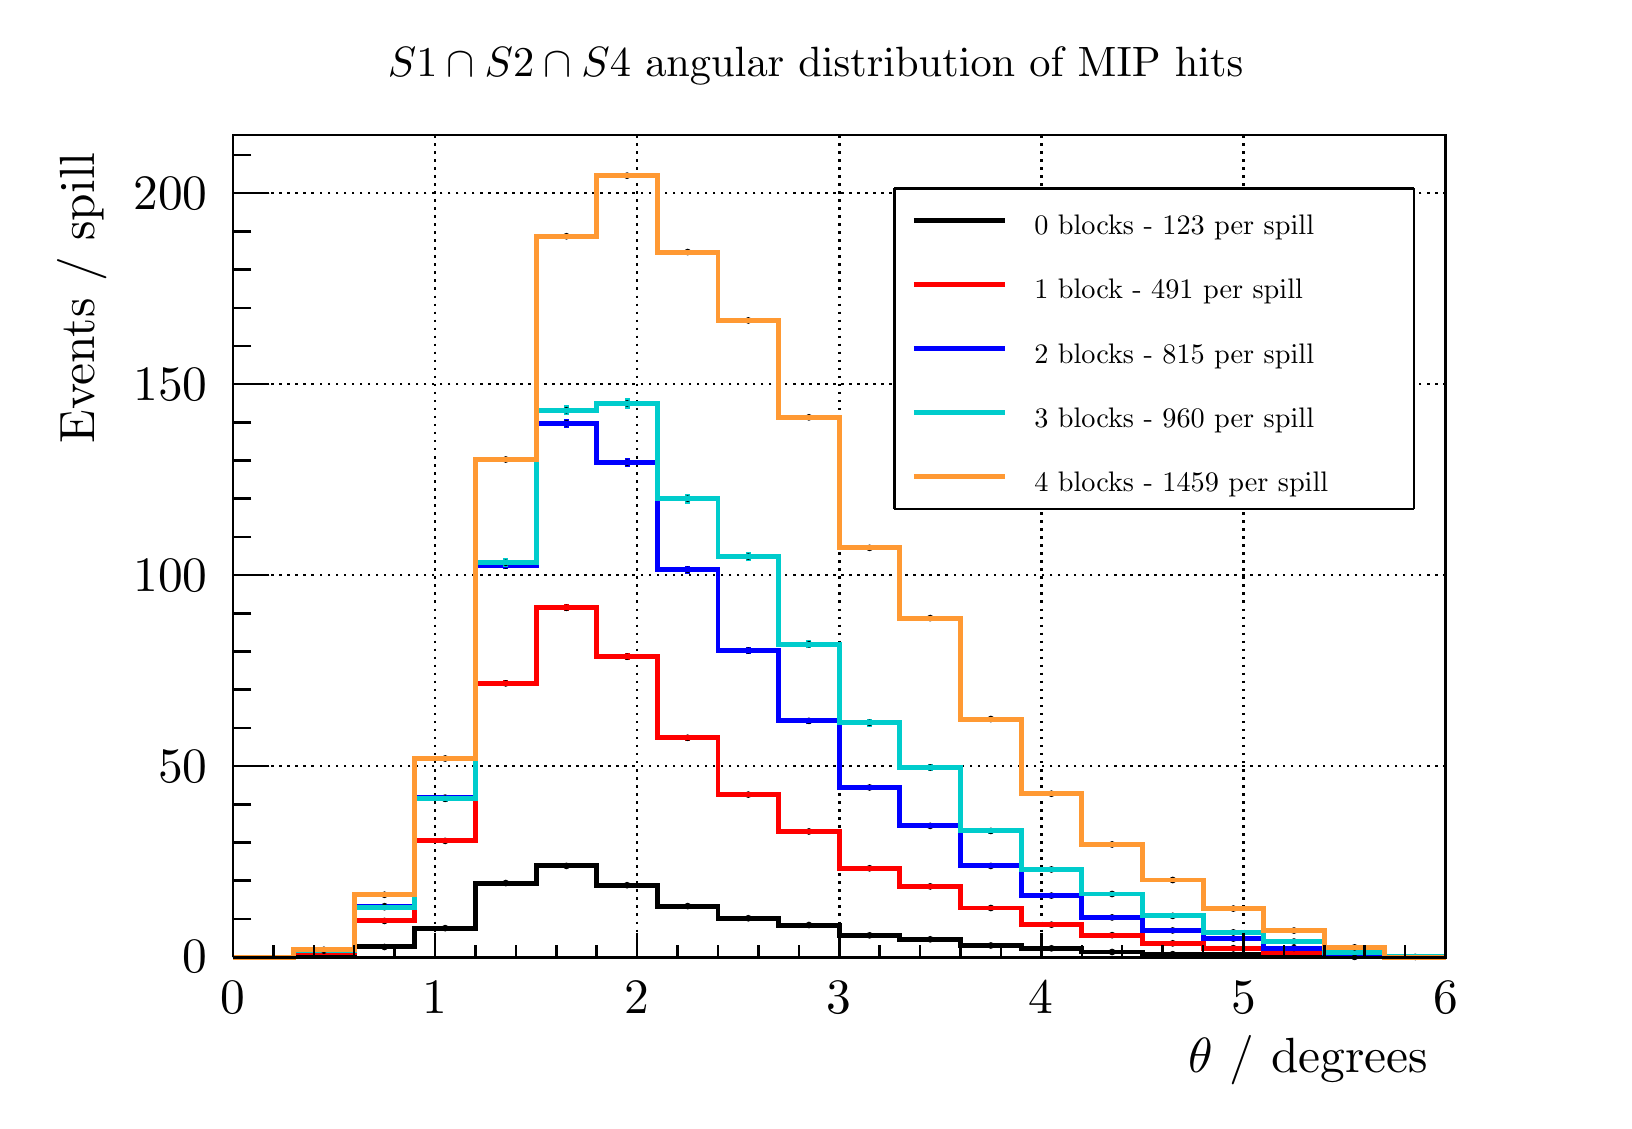
\begin{tikzpicture}
\pgfdeclareplotmark{cross} {
\pgfpathmoveto{\pgfpoint{-0.3\pgfplotmarksize}{\pgfplotmarksize}}
\pgfpathlineto{\pgfpoint{+0.3\pgfplotmarksize}{\pgfplotmarksize}}
\pgfpathlineto{\pgfpoint{+0.3\pgfplotmarksize}{0.3\pgfplotmarksize}}
\pgfpathlineto{\pgfpoint{+1\pgfplotmarksize}{0.3\pgfplotmarksize}}
\pgfpathlineto{\pgfpoint{+1\pgfplotmarksize}{-0.3\pgfplotmarksize}}
\pgfpathlineto{\pgfpoint{+0.3\pgfplotmarksize}{-0.3\pgfplotmarksize}}
\pgfpathlineto{\pgfpoint{+0.3\pgfplotmarksize}{-1.\pgfplotmarksize}}
\pgfpathlineto{\pgfpoint{-0.3\pgfplotmarksize}{-1.\pgfplotmarksize}}
\pgfpathlineto{\pgfpoint{-0.3\pgfplotmarksize}{-0.3\pgfplotmarksize}}
\pgfpathlineto{\pgfpoint{-1.\pgfplotmarksize}{-0.3\pgfplotmarksize}}
\pgfpathlineto{\pgfpoint{-1.\pgfplotmarksize}{0.3\pgfplotmarksize}}
\pgfpathlineto{\pgfpoint{-0.3\pgfplotmarksize}{0.3\pgfplotmarksize}}
\pgfpathclose
\pgfusepathqstroke
}
\pgfdeclareplotmark{cross*} {
\pgfpathmoveto{\pgfpoint{-0.3\pgfplotmarksize}{\pgfplotmarksize}}
\pgfpathlineto{\pgfpoint{+0.3\pgfplotmarksize}{\pgfplotmarksize}}
\pgfpathlineto{\pgfpoint{+0.3\pgfplotmarksize}{0.3\pgfplotmarksize}}
\pgfpathlineto{\pgfpoint{+1\pgfplotmarksize}{0.3\pgfplotmarksize}}
\pgfpathlineto{\pgfpoint{+1\pgfplotmarksize}{-0.3\pgfplotmarksize}}
\pgfpathlineto{\pgfpoint{+0.3\pgfplotmarksize}{-0.3\pgfplotmarksize}}
\pgfpathlineto{\pgfpoint{+0.3\pgfplotmarksize}{-1.\pgfplotmarksize}}
\pgfpathlineto{\pgfpoint{-0.3\pgfplotmarksize}{-1.\pgfplotmarksize}}
\pgfpathlineto{\pgfpoint{-0.3\pgfplotmarksize}{-0.3\pgfplotmarksize}}
\pgfpathlineto{\pgfpoint{-1.\pgfplotmarksize}{-0.3\pgfplotmarksize}}
\pgfpathlineto{\pgfpoint{-1.\pgfplotmarksize}{0.3\pgfplotmarksize}}
\pgfpathlineto{\pgfpoint{-0.3\pgfplotmarksize}{0.3\pgfplotmarksize}}
\pgfpathclose
\pgfusepathqfillstroke
}
\pgfdeclareplotmark{newstar} {
\pgfpathmoveto{\pgfqpoint{0pt}{\pgfplotmarksize}}
\pgfpathlineto{\pgfqpointpolar{44}{0.5\pgfplotmarksize}}
\pgfpathlineto{\pgfqpointpolar{18}{\pgfplotmarksize}}
\pgfpathlineto{\pgfqpointpolar{-20}{0.5\pgfplotmarksize}}
\pgfpathlineto{\pgfqpointpolar{-54}{\pgfplotmarksize}}
\pgfpathlineto{\pgfqpointpolar{-90}{0.5\pgfplotmarksize}}
\pgfpathlineto{\pgfqpointpolar{234}{\pgfplotmarksize}}
\pgfpathlineto{\pgfqpointpolar{198}{0.5\pgfplotmarksize}}
\pgfpathlineto{\pgfqpointpolar{162}{\pgfplotmarksize}}
\pgfpathlineto{\pgfqpointpolar{134}{0.5\pgfplotmarksize}}
\pgfpathclose
\pgfusepathqstroke
}
\pgfdeclareplotmark{newstar*} {
\pgfpathmoveto{\pgfqpoint{0pt}{\pgfplotmarksize}}
\pgfpathlineto{\pgfqpointpolar{44}{0.5\pgfplotmarksize}}
\pgfpathlineto{\pgfqpointpolar{18}{\pgfplotmarksize}}
\pgfpathlineto{\pgfqpointpolar{-20}{0.5\pgfplotmarksize}}
\pgfpathlineto{\pgfqpointpolar{-54}{\pgfplotmarksize}}
\pgfpathlineto{\pgfqpointpolar{-90}{0.5\pgfplotmarksize}}
\pgfpathlineto{\pgfqpointpolar{234}{\pgfplotmarksize}}
\pgfpathlineto{\pgfqpointpolar{198}{0.5\pgfplotmarksize}}
\pgfpathlineto{\pgfqpointpolar{162}{\pgfplotmarksize}}
\pgfpathlineto{\pgfqpointpolar{134}{0.5\pgfplotmarksize}}
\pgfpathclose
\pgfusepathqfillstroke
}
\definecolor{c}{rgb}{1,1,1};
\draw [color=c, fill=c] (0,0) rectangle (20,13.5632);
\draw [color=c, fill=c] (2.6,1.76322) rectangle (18,12.2069);
\definecolor{c}{rgb}{0,0,0};
\draw [c,line width=0.9] (2.6,1.76322) -- (2.6,12.2069) -- (18,12.2069) -- (18,1.76322) -- (2.6,1.76322);
\definecolor{c}{rgb}{1,1,1};
\draw [color=c, fill=c] (2.6,1.76322) rectangle (18,12.2069);
\definecolor{c}{rgb}{0,0,0};
\draw [c,line width=0.9] (2.6,1.76322) -- (2.6,12.2069) -- (18,12.2069) -- (18,1.76322) -- (2.6,1.76322);
\draw [c,line width=0.9] (2.6,1.76322) -- (18,1.76322);
\draw [c,dotted,line width=0.9] (2.6,12.2069) -- (2.6,1.76322);
\draw [c,dotted,line width=0.9] (5.16667,12.2069) -- (5.16667,1.76322);
\draw [c,dotted,line width=0.9] (7.73333,12.2069) -- (7.73333,1.76322);
\draw [c,dotted,line width=0.9] (10.3,12.2069) -- (10.3,1.76322);
\draw [c,dotted,line width=0.9] (12.8667,12.2069) -- (12.8667,1.76322);
\draw [c,dotted,line width=0.9] (15.4333,12.2069) -- (15.4333,1.76322);
\draw [c,dotted,line width=0.9] (18,12.2069) -- (18,1.76322);
\draw [c,line width=0.9] (2.6,1.76322) -- (2.6,12.2069);
\draw [c,dotted,line width=0.9] (18,1.76744) -- (2.6,1.76744);
\draw [c,dotted,line width=0.9] (18,4.19259) -- (2.6,4.19259);
\draw [c,dotted,line width=0.9] (18,6.61774) -- (2.6,6.61774);
\draw [c,dotted,line width=0.9] (18,9.04289) -- (2.6,9.04289);
\draw [c,dotted,line width=0.9] (18,11.468) -- (2.6,11.468);
\draw [c,dotted,line width=0.9] (18,1.76744) -- (2.6,1.76744);
\draw [c,dotted,line width=0.9] (18,11.468) -- (2.6,11.468);
\definecolor{c}{rgb}{0,0,0.6};
\draw [c,line width=0.9] (2.6,1.76744) -- (3.37,1.76744) -- (3.37,1.76744) -- (4.14,1.76744) -- (4.14,1.76744) -- (4.91,1.76744) -- (4.91,1.76744) -- (5.68,1.76744) -- (5.68,1.76744) -- (6.45,1.76744) -- (6.45,1.76744) -- (7.22,1.76744) --
 (7.22,1.76744) -- (7.99,1.76744) -- (7.99,1.76744) -- (8.76,1.76744) -- (8.76,1.76744) -- (9.53,1.76744) -- (9.53,1.76744) -- (10.3,1.76744) -- (10.3,1.76744) -- (11.07,1.76744) -- (11.07,1.76744) -- (11.84,1.76744) -- (11.84,1.76744) --
 (12.61,1.76744) -- (12.61,1.76744) -- (13.38,1.76744) -- (13.38,1.76744) -- (14.15,1.76744) -- (14.15,1.76744) -- (14.92,1.76744) -- (14.92,1.76744) -- (15.69,1.76744) -- (15.69,1.76744) -- (16.46,1.76744) -- (16.46,1.76744) -- (17.23,1.76744) --
 (17.23,1.76744) -- (18,1.76744);
\definecolor{c}{rgb}{0,0,0};
\draw [c,line width=0.9] (2.6,1.76322) -- (18,1.76322);
\draw [anchor= east] (18,0.461149) node[scale=1.78699, color=c, rotate=0]{$\theta$ / degrees};
\draw [c,line width=0.9] (2.6,2.07653) -- (2.6,1.76322);
\draw [c,line width=0.9] (3.11333,1.91987) -- (3.11333,1.76322);
\draw [c,line width=0.9] (3.62667,1.91987) -- (3.62667,1.76322);
\draw [c,line width=0.9] (4.14,1.91987) -- (4.14,1.76322);
\draw [c,line width=0.9] (4.65333,1.91987) -- (4.65333,1.76322);
\draw [c,line width=0.9] (5.16667,2.07653) -- (5.16667,1.76322);
\draw [c,line width=0.9] (5.68,1.91987) -- (5.68,1.76322);
\draw [c,line width=0.9] (6.19333,1.91987) -- (6.19333,1.76322);
\draw [c,line width=0.9] (6.70667,1.91987) -- (6.70667,1.76322);
\draw [c,line width=0.9] (7.22,1.91987) -- (7.22,1.76322);
\draw [c,line width=0.9] (7.73333,2.07653) -- (7.73333,1.76322);
\draw [c,line width=0.9] (8.24667,1.91987) -- (8.24667,1.76322);
\draw [c,line width=0.9] (8.76,1.91987) -- (8.76,1.76322);
\draw [c,line width=0.9] (9.27333,1.91987) -- (9.27333,1.76322);
\draw [c,line width=0.9] (9.78667,1.91987) -- (9.78667,1.76322);
\draw [c,line width=0.9] (10.3,2.07653) -- (10.3,1.76322);
\draw [c,line width=0.9] (10.8133,1.91987) -- (10.8133,1.76322);
\draw [c,line width=0.9] (11.3267,1.91987) -- (11.3267,1.76322);
\draw [c,line width=0.9] (11.84,1.91987) -- (11.84,1.76322);
\draw [c,line width=0.9] (12.3533,1.91987) -- (12.3533,1.76322);
\draw [c,line width=0.9] (12.8667,2.07653) -- (12.8667,1.76322);
\draw [c,line width=0.9] (13.38,1.91987) -- (13.38,1.76322);
\draw [c,line width=0.9] (13.8933,1.91987) -- (13.8933,1.76322);
\draw [c,line width=0.9] (14.4067,1.91987) -- (14.4067,1.76322);
\draw [c,line width=0.9] (14.92,1.91987) -- (14.92,1.76322);
\draw [c,line width=0.9] (15.4333,2.07653) -- (15.4333,1.76322);
\draw [c,line width=0.9] (15.9467,1.91987) -- (15.9467,1.76322);
\draw [c,line width=0.9] (16.46,1.91987) -- (16.46,1.76322);
\draw [c,line width=0.9] (16.9733,1.91987) -- (16.9733,1.76322);
\draw [c,line width=0.9] (17.4867,1.91987) -- (17.4867,1.76322);
\draw [c,line width=0.9] (18,2.07653) -- (18,1.76322);
\draw [anchor=base] (2.6,1.04437) node[scale=1.78699, color=c, rotate=0]{0};
\draw [anchor=base] (5.16667,1.04437) node[scale=1.78699, color=c, rotate=0]{1};
\draw [anchor=base] (7.73333,1.04437) node[scale=1.78699, color=c, rotate=0]{2};
\draw [anchor=base] (10.3,1.04437) node[scale=1.78699, color=c, rotate=0]{3};
\draw [anchor=base] (12.8667,1.04437) node[scale=1.78699, color=c, rotate=0]{4};
\draw [anchor=base] (15.4333,1.04437) node[scale=1.78699, color=c, rotate=0]{5};
\draw [anchor=base] (18,1.04437) node[scale=1.78699, color=c, rotate=0]{6};
\draw [c,line width=0.9] (2.6,1.76322) -- (2.6,12.2069);
\draw [anchor= east] (0.68,12.2069) node[scale=1.78699, color=c, rotate=90]{ Events / spill};
\draw [c,line width=0.9] (3.062,1.76744) -- (2.6,1.76744);
\draw [c,line width=0.9] (2.831,2.25247) -- (2.6,2.25247);
\draw [c,line width=0.9] (2.831,2.7375) -- (2.6,2.7375);
\draw [c,line width=0.9] (2.831,3.22253) -- (2.6,3.22253);
\draw [c,line width=0.9] (2.831,3.70756) -- (2.6,3.70756);
\draw [c,line width=0.9] (3.062,4.19259) -- (2.6,4.19259);
\draw [c,line width=0.9] (2.831,4.67762) -- (2.6,4.67762);
\draw [c,line width=0.9] (2.831,5.16265) -- (2.6,5.16265);
\draw [c,line width=0.9] (2.831,5.64768) -- (2.6,5.64768);
\draw [c,line width=0.9] (2.831,6.13271) -- (2.6,6.13271);
\draw [c,line width=0.9] (3.062,6.61774) -- (2.6,6.61774);
\draw [c,line width=0.9] (2.831,7.10277) -- (2.6,7.10277);
\draw [c,line width=0.9] (2.831,7.5878) -- (2.6,7.5878);
\draw [c,line width=0.9] (2.831,8.07283) -- (2.6,8.07283);
\draw [c,line width=0.9] (2.831,8.55786) -- (2.6,8.55786);
\draw [c,line width=0.9] (3.062,9.04289) -- (2.6,9.04289);
\draw [c,line width=0.9] (2.831,9.52792) -- (2.6,9.52792);
\draw [c,line width=0.9] (2.831,10.0129) -- (2.6,10.0129);
\draw [c,line width=0.9] (2.831,10.498) -- (2.6,10.498);
\draw [c,line width=0.9] (2.831,10.983) -- (2.6,10.983);
\draw [c,line width=0.9] (3.062,11.468) -- (2.6,11.468);
\draw [c,line width=0.9] (3.062,1.76744) -- (2.6,1.76744);
\draw [c,line width=0.9] (3.062,11.468) -- (2.6,11.468);
\draw [c,line width=0.9] (2.831,11.9531) -- (2.6,11.9531);
\draw [anchor= east] (2.5,1.76744) node[scale=1.78699, color=c, rotate=0]{0};
\draw [anchor= east] (2.5,4.19259) node[scale=1.78699, color=c, rotate=0]{50};
\draw [anchor= east] (2.5,6.61774) node[scale=1.78699, color=c, rotate=0]{100};
\draw [anchor= east] (2.5,9.04289) node[scale=1.78699, color=c, rotate=0]{150};
\draw [anchor= east] (2.5,11.468) node[scale=1.78699, color=c, rotate=0]{200};
\draw [c,line width=1.8] (3.755,1.78983) -- (3.755,1.79436);
\draw [c,line width=1.8] (3.755,1.79436) -- (3.755,1.79889);
\foreach \P in {(3.755,1.79436)}{\draw[mark options={color=c,fill=c},mark size=2.402402pt,mark=*,mark size=1pt] plot coordinates {\P};}
\draw [c,line width=1.8] (4.525,1.88561) -- (4.525,1.89499);
\draw [c,line width=1.8] (4.525,1.89499) -- (4.525,1.90437);
\foreach \P in {(4.525,1.89499)}{\draw[mark options={color=c,fill=c},mark size=2.402402pt,mark=*,mark size=1pt] plot coordinates {\P};}
\draw [c,line width=1.8] (5.295,2.11945) -- (5.295,2.13418);
\draw [c,line width=1.8] (5.295,2.13418) -- (5.295,2.14891);
\foreach \P in {(5.295,2.13418)}{\draw[mark options={color=c,fill=c},mark size=2.402402pt,mark=*,mark size=1pt] plot coordinates {\P};}
\draw [c,line width=1.8] (6.065,2.68461) -- (6.065,2.70679);
\draw [c,line width=1.8] (6.065,2.70679) -- (6.065,2.72898);
\foreach \P in {(6.065,2.70679)}{\draw[mark options={color=c,fill=c},mark size=2.402402pt,mark=*,mark size=1pt] plot coordinates {\P};}
\draw [c,line width=1.8] (6.835,2.9007) -- (6.835,2.92469);
\draw [c,line width=1.8] (6.835,2.92469) -- (6.835,2.94868);
\foreach \P in {(6.835,2.92469)}{\draw[mark options={color=c,fill=c},mark size=2.402402pt,mark=*,mark size=1pt] plot coordinates {\P};}
\draw [c,line width=1.8] (7.605,2.65802) -- (7.605,2.67959);
\draw [c,line width=1.8] (7.605,2.67959) -- (7.605,2.70116);
\foreach \P in {(7.605,2.67959)}{\draw[mark options={color=c,fill=c},mark size=2.402402pt,mark=*,mark size=1pt] plot coordinates {\P};}
\draw [c,line width=1.8] (8.375,2.39545) -- (8.375,2.41427);
\draw [c,line width=1.8] (8.375,2.41427) -- (8.375,2.4331);
\foreach \P in {(8.375,2.41427)}{\draw[mark options={color=c,fill=c},mark size=2.402402pt,mark=*,mark size=1pt] plot coordinates {\P};}
\draw [c,line width=1.8] (9.145,2.24317) -- (9.145,2.25985);
\draw [c,line width=1.8] (9.145,2.25985) -- (9.145,2.27654);
\foreach \P in {(9.145,2.25985)}{\draw[mark options={color=c,fill=c},mark size=2.402402pt,mark=*,mark size=1pt] plot coordinates {\P};}
\draw [c,line width=1.8] (9.915,2.15841) -- (9.915,2.17379);
\draw [c,line width=1.8] (9.915,2.17379) -- (9.915,2.18916);
\foreach \P in {(9.915,2.17379)}{\draw[mark options={color=c,fill=c},mark size=2.402402pt,mark=*,mark size=1pt] plot coordinates {\P};}
\draw [c,line width=1.8] (10.685,2.02998) -- (10.685,2.04288);
\draw [c,line width=1.8] (10.685,2.04288) -- (10.685,2.05579);
\foreach \P in {(10.685,2.04288)}{\draw[mark options={color=c,fill=c},mark size=2.402402pt,mark=*,mark size=1pt] plot coordinates {\P};}
\draw [c,line width=1.8] (11.455,1.9807) -- (11.455,1.99236);
\draw [c,line width=1.8] (11.455,1.99236) -- (11.455,2.00403);
\foreach \P in {(11.455,1.99236)}{\draw[mark options={color=c,fill=c},mark size=2.402402pt,mark=*,mark size=1pt] plot coordinates {\P};}
\draw [c,line width=1.8] (12.225,1.90443) -- (12.225,1.91395);
\draw [c,line width=1.8] (12.225,1.91395) -- (12.225,1.92347);
\foreach \P in {(12.225,1.91395)}{\draw[mark options={color=c,fill=c},mark size=2.402402pt,mark=*,mark size=1pt] plot coordinates {\P};}
\draw [c,line width=1.8] (12.995,1.86923) -- (12.995,1.87784);
\draw [c,line width=1.8] (12.995,1.87784) -- (12.995,1.88644);
\foreach \P in {(12.995,1.87784)}{\draw[mark options={color=c,fill=c},mark size=2.402402pt,mark=*,mark size=1pt] plot coordinates {\P};}
\draw [c,line width=1.8] (13.765,1.82465) -- (13.765,1.83133);
\draw [c,line width=1.8] (13.765,1.83133) -- (13.765,1.83801);
\foreach \P in {(13.765,1.83133)}{\draw[mark options={color=c,fill=c},mark size=2.402402pt,mark=*,mark size=1pt] plot coordinates {\P};}
\draw [c,line width=1.8] (14.535,1.79842) -- (14.535,1.80368);
\draw [c,line width=1.8] (14.535,1.80368) -- (14.535,1.80894);
\foreach \P in {(14.535,1.80368)}{\draw[mark options={color=c,fill=c},mark size=2.402402pt,mark=*,mark size=1pt] plot coordinates {\P};}
\draw [c,line width=1.8] (15.305,1.79286) -- (15.305,1.79794);
\draw [c,line width=1.8] (15.305,1.79794) -- (15.305,1.80301);
\foreach \P in {(15.305,1.79794)}{\draw[mark options={color=c,fill=c},mark size=2.402402pt,mark=*,mark size=1pt] plot coordinates {\P};}
\draw [c,line width=1.8] (16.075,1.7812) -- (16.075,1.78518);
\draw [c,line width=1.8] (16.075,1.78518) -- (16.075,1.78916);
\foreach \P in {(16.075,1.78518)}{\draw[mark options={color=c,fill=c},mark size=2.402402pt,mark=*,mark size=1pt] plot coordinates {\P};}
\draw [c,line width=1.8] (16.845,1.76709) -- (16.845,1.76925);
\draw [c,line width=1.8] (16.845,1.76925) -- (16.845,1.77141);
\foreach \P in {(16.845,1.76925)}{\draw[mark options={color=c,fill=c},mark size=2.402402pt,mark=*,mark size=1pt] plot coordinates {\P};}
\draw [c,line width=1.8] (2.6,1.76744) -- (3.37,1.76744) -- (3.37,1.79436) -- (4.14,1.79436) -- (4.14,1.89499) -- (4.91,1.89499) -- (4.91,2.13418) -- (5.68,2.13418) -- (5.68,2.70679) -- (6.45,2.70679) -- (6.45,2.92469) -- (7.22,2.92469) --
 (7.22,2.67959) -- (7.99,2.67959) -- (7.99,2.41427) -- (8.76,2.41427) -- (8.76,2.25985) -- (9.53,2.25985) -- (9.53,2.17379) -- (10.3,2.17379) -- (10.3,2.04288) -- (11.07,2.04288) -- (11.07,1.99236) -- (11.84,1.99236) -- (11.84,1.91395) --
 (12.61,1.91395) -- (12.61,1.87784) -- (13.38,1.87784) -- (13.38,1.83133) -- (14.15,1.83133) -- (14.15,1.80368) -- (14.92,1.80368) -- (14.92,1.79794) -- (15.69,1.79794) -- (15.69,1.78518) -- (16.46,1.78518) -- (16.46,1.76925) -- (17.23,1.76925) --
 (17.23,1.76744) -- (18,1.76744);
\definecolor{c}{rgb}{1,0,0};
\draw [c,line width=1.8] (3.755,1.81396) -- (3.755,1.81942);
\draw [c,line width=1.8] (3.755,1.81942) -- (3.755,1.82488);
\definecolor{c}{rgb}{0,0,0};
\foreach \P in {(3.755,1.81942)}{\draw[mark options={color=c,fill=c},mark size=2.402402pt,mark=*,mark size=1pt] plot coordinates {\P};}
\definecolor{c}{rgb}{1,0,0};
\draw [c,line width=1.8] (4.525,2.21057) -- (4.525,2.22581);
\draw [c,line width=1.8] (4.525,2.22581) -- (4.525,2.24106);
\definecolor{c}{rgb}{0,0,0};
\foreach \P in {(4.525,2.22581)}{\draw[mark options={color=c,fill=c},mark size=2.402402pt,mark=*,mark size=1pt] plot coordinates {\P};}
\definecolor{c}{rgb}{1,0,0};
\draw [c,line width=1.8] (5.295,3.21613) -- (5.295,3.24228);
\draw [c,line width=1.8] (5.295,3.24228) -- (5.295,3.26842);
\definecolor{c}{rgb}{0,0,0};
\foreach \P in {(5.295,3.24228)}{\draw[mark options={color=c,fill=c},mark size=2.402402pt,mark=*,mark size=1pt] plot coordinates {\P};}
\definecolor{c}{rgb}{1,0,0};
\draw [c,line width=1.8] (6.065,5.20308) -- (6.065,5.24251);
\draw [c,line width=1.8] (6.065,5.24251) -- (6.065,5.28193);
\definecolor{c}{rgb}{0,0,0};
\foreach \P in {(6.065,5.24251)}{\draw[mark options={color=c,fill=c},mark size=2.402402pt,mark=*,mark size=1pt] plot coordinates {\P};}
\definecolor{c}{rgb}{1,0,0};
\draw [c,line width=1.8] (6.835,6.15816) -- (6.835,6.20243);
\draw [c,line width=1.8] (6.835,6.20243) -- (6.835,6.24669);
\definecolor{c}{rgb}{0,0,0};
\foreach \P in {(6.835,6.20243)}{\draw[mark options={color=c,fill=c},mark size=2.402402pt,mark=*,mark size=1pt] plot coordinates {\P};}
\definecolor{c}{rgb}{1,0,0};
\draw [c,line width=1.8] (7.605,5.5402) -- (7.605,5.58196);
\draw [c,line width=1.8] (7.605,5.58196) -- (7.605,5.62371);
\definecolor{c}{rgb}{0,0,0};
\foreach \P in {(7.605,5.58196)}{\draw[mark options={color=c,fill=c},mark size=2.402402pt,mark=*,mark size=1pt] plot coordinates {\P};}
\definecolor{c}{rgb}{1,0,0};
\draw [c,line width=1.8] (8.375,4.51598) -- (8.375,4.55208);
\draw [c,line width=1.8] (8.375,4.55208) -- (8.375,4.58817);
\definecolor{c}{rgb}{0,0,0};
\foreach \P in {(8.375,4.55208)}{\draw[mark options={color=c,fill=c},mark size=2.402402pt,mark=*,mark size=1pt] plot coordinates {\P};}
\definecolor{c}{rgb}{1,0,0};
\draw [c,line width=1.8] (9.145,3.79835) -- (9.145,3.83014);
\draw [c,line width=1.8] (9.145,3.83014) -- (9.145,3.86192);
\definecolor{c}{rgb}{0,0,0};
\foreach \P in {(9.145,3.83014)}{\draw[mark options={color=c,fill=c},mark size=2.402402pt,mark=*,mark size=1pt] plot coordinates {\P};}
\definecolor{c}{rgb}{1,0,0};
\draw [c,line width=1.8] (9.915,3.33388) -- (9.915,3.36201);
\draw [c,line width=1.8] (9.915,3.36201) -- (9.915,3.39015);
\definecolor{c}{rgb}{0,0,0};
\foreach \P in {(9.915,3.36201)}{\draw[mark options={color=c,fill=c},mark size=2.402402pt,mark=*,mark size=1pt] plot coordinates {\P};}
\definecolor{c}{rgb}{1,0,0};
\draw [c,line width=1.8] (10.685,2.87003) -- (10.685,2.89427);
\draw [c,line width=1.8] (10.685,2.89427) -- (10.685,2.91852);
\definecolor{c}{rgb}{0,0,0};
\foreach \P in {(10.685,2.89427)}{\draw[mark options={color=c,fill=c},mark size=2.402402pt,mark=*,mark size=1pt] plot coordinates {\P};}
\definecolor{c}{rgb}{1,0,0};
\draw [c,line width=1.8] (11.455,2.64248) -- (11.455,2.66431);
\draw [c,line width=1.8] (11.455,2.66431) -- (11.455,2.68613);
\definecolor{c}{rgb}{0,0,0};
\foreach \P in {(11.455,2.66431)}{\draw[mark options={color=c,fill=c},mark size=2.402402pt,mark=*,mark size=1pt] plot coordinates {\P};}
\definecolor{c}{rgb}{1,0,0};
\draw [c,line width=1.8] (12.225,2.37137) -- (12.225,2.38992);
\draw [c,line width=1.8] (12.225,2.38992) -- (12.225,2.40847);
\definecolor{c}{rgb}{0,0,0};
\foreach \P in {(12.225,2.38992)}{\draw[mark options={color=c,fill=c},mark size=2.402402pt,mark=*,mark size=1pt] plot coordinates {\P};}
\definecolor{c}{rgb}{1,0,0};
\draw [c,line width=1.8] (12.995,2.16257) -- (12.995,2.17821);
\draw [c,line width=1.8] (12.995,2.17821) -- (12.995,2.19386);
\definecolor{c}{rgb}{0,0,0};
\foreach \P in {(12.995,2.17821)}{\draw[mark options={color=c,fill=c},mark size=2.402402pt,mark=*,mark size=1pt] plot coordinates {\P};}
\definecolor{c}{rgb}{1,0,0};
\draw [c,line width=1.8] (13.765,2.0315) -- (13.765,2.04493);
\draw [c,line width=1.8] (13.765,2.04493) -- (13.765,2.05836);
\definecolor{c}{rgb}{0,0,0};
\foreach \P in {(13.765,2.04493)}{\draw[mark options={color=c,fill=c},mark size=2.402402pt,mark=*,mark size=1pt] plot coordinates {\P};}
\definecolor{c}{rgb}{1,0,0};
\draw [c,line width=1.8] (14.535,1.93052) -- (14.535,1.94126);
\draw [c,line width=1.8] (14.535,1.94126) -- (14.535,1.952);
\definecolor{c}{rgb}{0,0,0};
\foreach \P in {(14.535,1.94126)}{\draw[mark options={color=c,fill=c},mark size=2.402402pt,mark=*,mark size=1pt] plot coordinates {\P};}
\definecolor{c}{rgb}{1,0,0};
\draw [c,line width=1.8] (15.305,1.87034) -- (15.305,1.87956);
\draw [c,line width=1.8] (15.305,1.87956) -- (15.305,1.88878);
\definecolor{c}{rgb}{0,0,0};
\foreach \P in {(15.305,1.87956)}{\draw[mark options={color=c,fill=c},mark size=2.402402pt,mark=*,mark size=1pt] plot coordinates {\P};}
\definecolor{c}{rgb}{1,0,0};
\draw [c,line width=1.8] (16.075,1.82261) -- (16.075,1.8304);
\draw [c,line width=1.8] (16.075,1.8304) -- (16.075,1.8382);
\definecolor{c}{rgb}{0,0,0};
\foreach \P in {(16.075,1.8304)}{\draw[mark options={color=c,fill=c},mark size=2.402402pt,mark=*,mark size=1pt] plot coordinates {\P};}
\definecolor{c}{rgb}{1,0,0};
\draw [c,line width=1.8] (16.845,1.77091) -- (16.845,1.77506);
\draw [c,line width=1.8] (16.845,1.77506) -- (16.845,1.77922);
\definecolor{c}{rgb}{0,0,0};
\foreach \P in {(16.845,1.77506)}{\draw[mark options={color=c,fill=c},mark size=2.402402pt,mark=*,mark size=1pt] plot coordinates {\P};}
\definecolor{c}{rgb}{1,0,0};
\draw [c,line width=1.8] (2.6,1.76744) -- (3.37,1.76744) -- (3.37,1.81942) -- (4.14,1.81942) -- (4.14,2.22581) -- (4.91,2.22581) -- (4.91,3.24228) -- (5.68,3.24228) -- (5.68,5.24251) -- (6.45,5.24251) -- (6.45,6.20243) -- (7.22,6.20243) --
 (7.22,5.58196) -- (7.99,5.58196) -- (7.99,4.55208) -- (8.76,4.55208) -- (8.76,3.83014) -- (9.53,3.83014) -- (9.53,3.36201) -- (10.3,3.36201) -- (10.3,2.89427) -- (11.07,2.89427) -- (11.07,2.66431) -- (11.84,2.66431) -- (11.84,2.38992) --
 (12.61,2.38992) -- (12.61,2.17821) -- (13.38,2.17821) -- (13.38,2.04493) -- (14.15,2.04493) -- (14.15,1.94126) -- (14.92,1.94126) -- (14.92,1.87956) -- (15.69,1.87956) -- (15.69,1.8304) -- (16.46,1.8304) -- (16.46,1.77506) -- (17.23,1.77506) --
 (17.23,1.76744) -- (18,1.76744);
\definecolor{c}{rgb}{0,0,1};
\draw [c,line width=1.8] (3.755,1.84408) -- (3.755,1.85134);
\draw [c,line width=1.8] (3.755,1.85134) -- (3.755,1.8586);
\definecolor{c}{rgb}{0,0,0};
\foreach \P in {(3.755,1.85134)}{\draw[mark options={color=c,fill=c},mark size=2.402402pt,mark=*,mark size=1pt] plot coordinates {\P};}
\definecolor{c}{rgb}{0,0,1};
\draw [c,line width=1.8] (4.525,2.39435) -- (4.525,2.41302);
\draw [c,line width=1.8] (4.525,2.41302) -- (4.525,2.43169);
\definecolor{c}{rgb}{0,0,0};
\foreach \P in {(4.525,2.41302)}{\draw[mark options={color=c,fill=c},mark size=2.402402pt,mark=*,mark size=1pt] plot coordinates {\P};}
\definecolor{c}{rgb}{0,0,1};
\draw [c,line width=1.8] (5.295,3.76008) -- (5.295,3.79169);
\draw [c,line width=1.8] (5.295,3.79169) -- (5.295,3.82329);
\definecolor{c}{rgb}{0,0,0};
\foreach \P in {(5.295,3.79169)}{\draw[mark options={color=c,fill=c},mark size=2.402402pt,mark=*,mark size=1pt] plot coordinates {\P};}
\definecolor{c}{rgb}{0,0,1};
\draw [c,line width=1.8] (6.065,6.68987) -- (6.065,6.73794);
\draw [c,line width=1.8] (6.065,6.73794) -- (6.065,6.78601);
\definecolor{c}{rgb}{0,0,0};
\foreach \P in {(6.065,6.73794)}{\draw[mark options={color=c,fill=c},mark size=2.402402pt,mark=*,mark size=1pt] plot coordinates {\P};}
\definecolor{c}{rgb}{0,0,1};
\draw [c,line width=1.8] (6.835,8.49075) -- (6.835,8.54602);
\draw [c,line width=1.8] (6.835,8.54602) -- (6.835,8.60129);
\definecolor{c}{rgb}{0,0,0};
\foreach \P in {(6.835,8.54602)}{\draw[mark options={color=c,fill=c},mark size=2.402402pt,mark=*,mark size=1pt] plot coordinates {\P};}
\definecolor{c}{rgb}{0,0,1};
\draw [c,line width=1.8] (7.605,7.9918) -- (7.605,8.04532);
\draw [c,line width=1.8] (7.605,8.04532) -- (7.605,8.09884);
\definecolor{c}{rgb}{0,0,0};
\foreach \P in {(7.605,8.04532)}{\draw[mark options={color=c,fill=c},mark size=2.402402pt,mark=*,mark size=1pt] plot coordinates {\P};}
\definecolor{c}{rgb}{0,0,1};
\draw [c,line width=1.8] (8.375,6.63685) -- (8.375,6.68509);
\draw [c,line width=1.8] (8.375,6.68509) -- (8.375,6.73333);
\definecolor{c}{rgb}{0,0,0};
\foreach \P in {(8.375,6.68509)}{\draw[mark options={color=c,fill=c},mark size=2.402402pt,mark=*,mark size=1pt] plot coordinates {\P};}
\definecolor{c}{rgb}{0,0,1};
\draw [c,line width=1.8] (9.145,5.61567) -- (9.145,5.65956);
\draw [c,line width=1.8] (9.145,5.65956) -- (9.145,5.70345);
\definecolor{c}{rgb}{0,0,0};
\foreach \P in {(9.145,5.65956)}{\draw[mark options={color=c,fill=c},mark size=2.402402pt,mark=*,mark size=1pt] plot coordinates {\P};}
\definecolor{c}{rgb}{0,0,1};
\draw [c,line width=1.8] (9.915,4.72777) -- (9.915,4.76661);
\draw [c,line width=1.8] (9.915,4.76661) -- (9.915,4.80545);
\definecolor{c}{rgb}{0,0,0};
\foreach \P in {(9.915,4.76661)}{\draw[mark options={color=c,fill=c},mark size=2.402402pt,mark=*,mark size=1pt] plot coordinates {\P};}
\definecolor{c}{rgb}{0,0,1};
\draw [c,line width=1.8] (10.685,3.88714) -- (10.685,3.92086);
\draw [c,line width=1.8] (10.685,3.92086) -- (10.685,3.95458);
\definecolor{c}{rgb}{0,0,0};
\foreach \P in {(10.685,3.92086)}{\draw[mark options={color=c,fill=c},mark size=2.402402pt,mark=*,mark size=1pt] plot coordinates {\P};}
\definecolor{c}{rgb}{0,0,1};
\draw [c,line width=1.8] (11.455,3.40333) -- (11.455,3.43318);
\draw [c,line width=1.8] (11.455,3.43318) -- (11.455,3.46303);
\definecolor{c}{rgb}{0,0,0};
\foreach \P in {(11.455,3.43318)}{\draw[mark options={color=c,fill=c},mark size=2.402402pt,mark=*,mark size=1pt] plot coordinates {\P};}
\definecolor{c}{rgb}{0,0,1};
\draw [c,line width=1.8] (12.225,2.89917) -- (12.225,2.92452);
\draw [c,line width=1.8] (12.225,2.92452) -- (12.225,2.94987);
\definecolor{c}{rgb}{0,0,0};
\foreach \P in {(12.225,2.92452)}{\draw[mark options={color=c,fill=c},mark size=2.402402pt,mark=*,mark size=1pt] plot coordinates {\P};}
\definecolor{c}{rgb}{0,0,1};
\draw [c,line width=1.8] (12.995,2.52582) -- (12.995,2.54757);
\draw [c,line width=1.8] (12.995,2.54757) -- (12.995,2.56932);
\definecolor{c}{rgb}{0,0,0};
\foreach \P in {(12.995,2.54757)}{\draw[mark options={color=c,fill=c},mark size=2.402402pt,mark=*,mark size=1pt] plot coordinates {\P};}
\definecolor{c}{rgb}{0,0,1};
\draw [c,line width=1.8] (13.765,2.25214) -- (13.765,2.27022);
\draw [c,line width=1.8] (13.765,2.27022) -- (13.765,2.2883);
\definecolor{c}{rgb}{0,0,0};
\foreach \P in {(13.765,2.27022)}{\draw[mark options={color=c,fill=c},mark size=2.402402pt,mark=*,mark size=1pt] plot coordinates {\P};}
\definecolor{c}{rgb}{0,0,1};
\draw [c,line width=1.8] (14.535,2.08946) -- (14.535,2.10492);
\draw [c,line width=1.8] (14.535,2.10492) -- (14.535,2.12039);
\definecolor{c}{rgb}{0,0,0};
\foreach \P in {(14.535,2.10492)}{\draw[mark options={color=c,fill=c},mark size=2.402402pt,mark=*,mark size=1pt] plot coordinates {\P};}
\definecolor{c}{rgb}{0,0,1};
\draw [c,line width=1.8] (15.305,1.98767) -- (15.305,2.00128);
\draw [c,line width=1.8] (15.305,2.00128) -- (15.305,2.01488);
\definecolor{c}{rgb}{0,0,0};
\foreach \P in {(15.305,2.00128)}{\draw[mark options={color=c,fill=c},mark size=2.402402pt,mark=*,mark size=1pt] plot coordinates {\P};}
\definecolor{c}{rgb}{0,0,1};
\draw [c,line width=1.8] (16.075,1.87059) -- (16.075,1.88108);
\draw [c,line width=1.8] (16.075,1.88108) -- (16.075,1.89157);
\definecolor{c}{rgb}{0,0,0};
\foreach \P in {(16.075,1.88108)}{\draw[mark options={color=c,fill=c},mark size=2.402402pt,mark=*,mark size=1pt] plot coordinates {\P};}
\definecolor{c}{rgb}{0,0,1};
\draw [c,line width=1.8] (16.845,1.7943) -- (16.845,1.80135);
\draw [c,line width=1.8] (16.845,1.80135) -- (16.845,1.8084);
\definecolor{c}{rgb}{0,0,0};
\foreach \P in {(16.845,1.80135)}{\draw[mark options={color=c,fill=c},mark size=2.402402pt,mark=*,mark size=1pt] plot coordinates {\P};}
\definecolor{c}{rgb}{0,0,1};
\draw [c,line width=1.8] (2.6,1.76744) -- (3.37,1.76744) -- (3.37,1.85134) -- (4.14,1.85134) -- (4.14,2.41302) -- (4.91,2.41302) -- (4.91,3.79169) -- (5.68,3.79169) -- (5.68,6.73794) -- (6.45,6.73794) -- (6.45,8.54602) -- (7.22,8.54602) --
 (7.22,8.04532) -- (7.99,8.04532) -- (7.99,6.68509) -- (8.76,6.68509) -- (8.76,5.65956) -- (9.53,5.65956) -- (9.53,4.76661) -- (10.3,4.76661) -- (10.3,3.92086) -- (11.07,3.92086) -- (11.07,3.43318) -- (11.84,3.43318) -- (11.84,2.92452) --
 (12.61,2.92452) -- (12.61,2.54757) -- (13.38,2.54757) -- (13.38,2.27022) -- (14.15,2.27022) -- (14.15,2.10492) -- (14.92,2.10492) -- (14.92,2.00128) -- (15.69,2.00128) -- (15.69,1.88108) -- (16.46,1.88108) -- (16.46,1.80135) -- (17.23,1.80135) --
 (17.23,1.76744) -- (18,1.76744);
\definecolor{c}{rgb}{0,0.8,0.8};
\draw [c,line width=1.8] (3.755,1.84134) -- (3.755,1.84959);
\draw [c,line width=1.8] (3.755,1.84959) -- (3.755,1.85784);
\definecolor{c}{rgb}{0,0,0};
\foreach \P in {(3.755,1.84959)}{\draw[mark options={color=c,fill=c},mark size=2.402402pt,mark=*,mark size=1pt] plot coordinates {\P};}
\definecolor{c}{rgb}{0,0.8,0.8};
\draw [c,line width=1.8] (4.525,2.37933) -- (4.525,2.40063);
\draw [c,line width=1.8] (4.525,2.40063) -- (4.525,2.42192);
\definecolor{c}{rgb}{0,0,0};
\foreach \P in {(4.525,2.40063)}{\draw[mark options={color=c,fill=c},mark size=2.402402pt,mark=*,mark size=1pt] plot coordinates {\P};}
\definecolor{c}{rgb}{0,0.8,0.8};
\draw [c,line width=1.8] (5.295,3.74049) -- (5.295,3.77657);
\draw [c,line width=1.8] (5.295,3.77657) -- (5.295,3.81265);
\definecolor{c}{rgb}{0,0,0};
\foreach \P in {(5.295,3.77657)}{\draw[mark options={color=c,fill=c},mark size=2.402402pt,mark=*,mark size=1pt] plot coordinates {\P};}
\definecolor{c}{rgb}{0,0.8,0.8};
\draw [c,line width=1.8] (6.065,6.71858) -- (6.065,6.7739);
\draw [c,line width=1.8] (6.065,6.7739) -- (6.065,6.82921);
\definecolor{c}{rgb}{0,0,0};
\foreach \P in {(6.065,6.7739)}{\draw[mark options={color=c,fill=c},mark size=2.402402pt,mark=*,mark size=1pt] plot coordinates {\P};}
\definecolor{c}{rgb}{0,0.8,0.8};
\draw [c,line width=1.8] (6.835,8.64689) -- (6.835,8.71101);
\draw [c,line width=1.8] (6.835,8.71101) -- (6.835,8.77513);
\definecolor{c}{rgb}{0,0,0};
\foreach \P in {(6.835,8.71101)}{\draw[mark options={color=c,fill=c},mark size=2.402402pt,mark=*,mark size=1pt] plot coordinates {\P};}
\definecolor{c}{rgb}{0,0.8,0.8};
\draw [c,line width=1.8] (7.605,8.73228) -- (7.605,8.79806);
\draw [c,line width=1.8] (7.605,8.79806) -- (7.605,8.86384);
\definecolor{c}{rgb}{0,0,0};
\foreach \P in {(7.605,8.79806)}{\draw[mark options={color=c,fill=c},mark size=2.402402pt,mark=*,mark size=1pt] plot coordinates {\P};}
\definecolor{c}{rgb}{0,0.8,0.8};
\draw [c,line width=1.8] (8.375,7.52703) -- (8.375,7.58837);
\draw [c,line width=1.8] (8.375,7.58837) -- (8.375,7.6497);
\definecolor{c}{rgb}{0,0,0};
\foreach \P in {(8.375,7.58837)}{\draw[mark options={color=c,fill=c},mark size=2.402402pt,mark=*,mark size=1pt] plot coordinates {\P};}
\definecolor{c}{rgb}{0,0.8,0.8};
\draw [c,line width=1.8] (9.145,6.79362) -- (9.145,6.85271);
\draw [c,line width=1.8] (9.145,6.85271) -- (9.145,6.91179);
\definecolor{c}{rgb}{0,0,0};
\foreach \P in {(9.145,6.85271)}{\draw[mark options={color=c,fill=c},mark size=2.402402pt,mark=*,mark size=1pt] plot coordinates {\P};}
\definecolor{c}{rgb}{0,0.8,0.8};
\draw [c,line width=1.8] (9.915,5.68617) -- (9.915,5.73927);
\draw [c,line width=1.8] (9.915,5.73927) -- (9.915,5.79236);
\definecolor{c}{rgb}{0,0,0};
\foreach \P in {(9.915,5.73927)}{\draw[mark options={color=c,fill=c},mark size=2.402402pt,mark=*,mark size=1pt] plot coordinates {\P};}
\definecolor{c}{rgb}{0,0.8,0.8};
\draw [c,line width=1.8] (10.685,4.69497) -- (10.685,4.74204);
\draw [c,line width=1.8] (10.685,4.74204) -- (10.685,4.78911);
\definecolor{c}{rgb}{0,0,0};
\foreach \P in {(10.685,4.74204)}{\draw[mark options={color=c,fill=c},mark size=2.402402pt,mark=*,mark size=1pt] plot coordinates {\P};}
\definecolor{c}{rgb}{0,0.8,0.8};
\draw [c,line width=1.8] (11.455,4.13163) -- (11.455,4.17519);
\draw [c,line width=1.8] (11.455,4.17519) -- (11.455,4.21874);
\definecolor{c}{rgb}{0,0,0};
\foreach \P in {(11.455,4.17519)}{\draw[mark options={color=c,fill=c},mark size=2.402402pt,mark=*,mark size=1pt] plot coordinates {\P};}
\definecolor{c}{rgb}{0,0.8,0.8};
\draw [c,line width=1.8] (12.225,3.33326) -- (12.225,3.36898);
\draw [c,line width=1.8] (12.225,3.36898) -- (12.225,3.4047);
\definecolor{c}{rgb}{0,0,0};
\foreach \P in {(12.225,3.36898)}{\draw[mark options={color=c,fill=c},mark size=2.402402pt,mark=*,mark size=1pt] plot coordinates {\P};}
\definecolor{c}{rgb}{0,0.8,0.8};
\draw [c,line width=1.8] (12.995,2.84872) -- (12.995,2.87968);
\draw [c,line width=1.8] (12.995,2.87968) -- (12.995,2.91065);
\definecolor{c}{rgb}{0,0,0};
\foreach \P in {(12.995,2.87968)}{\draw[mark options={color=c,fill=c},mark size=2.402402pt,mark=*,mark size=1pt] plot coordinates {\P};}
\definecolor{c}{rgb}{0,0.8,0.8};
\draw [c,line width=1.8] (13.765,2.53969) -- (13.765,2.56783);
\draw [c,line width=1.8] (13.765,2.56783) -- (13.765,2.59596);
\definecolor{c}{rgb}{0,0,0};
\foreach \P in {(13.765,2.56783)}{\draw[mark options={color=c,fill=c},mark size=2.402402pt,mark=*,mark size=1pt] plot coordinates {\P};}
\definecolor{c}{rgb}{0,0.8,0.8};
\draw [c,line width=1.8] (14.535,2.26659) -- (14.535,2.29015);
\draw [c,line width=1.8] (14.535,2.29015) -- (14.535,2.3137);
\definecolor{c}{rgb}{0,0,0};
\foreach \P in {(14.535,2.29015)}{\draw[mark options={color=c,fill=c},mark size=2.402402pt,mark=*,mark size=1pt] plot coordinates {\P};}
\definecolor{c}{rgb}{0,0.8,0.8};
\draw [c,line width=1.8] (15.305,2.06072) -- (15.305,2.0804);
\draw [c,line width=1.8] (15.305,2.0804) -- (15.305,2.10008);
\definecolor{c}{rgb}{0,0,0};
\foreach \P in {(15.305,2.0804)}{\draw[mark options={color=c,fill=c},mark size=2.402402pt,mark=*,mark size=1pt] plot coordinates {\P};}
\definecolor{c}{rgb}{0,0.8,0.8};
\draw [c,line width=1.8] (16.075,1.94622) -- (16.075,1.96379);
\draw [c,line width=1.8] (16.075,1.96379) -- (16.075,1.98136);
\definecolor{c}{rgb}{0,0,0};
\foreach \P in {(16.075,1.96379)}{\draw[mark options={color=c,fill=c},mark size=2.402402pt,mark=*,mark size=1pt] plot coordinates {\P};}
\definecolor{c}{rgb}{0,0.8,0.8};
\draw [c,line width=1.8] (16.845,1.8084) -- (16.845,1.81884);
\draw [c,line width=1.8] (16.845,1.81884) -- (16.845,1.82929);
\definecolor{c}{rgb}{0,0,0};
\foreach \P in {(16.845,1.81884)}{\draw[mark options={color=c,fill=c},mark size=2.402402pt,mark=*,mark size=1pt] plot coordinates {\P};}
\definecolor{c}{rgb}{0,0.8,0.8};
\draw [c,line width=1.8] (17.615,1.76322) -- (17.615,1.76883);
\draw [c,line width=1.8] (17.615,1.76883) -- (17.615,1.77444);
\definecolor{c}{rgb}{0,0,0};
\foreach \P in {(17.615,1.76883)}{\draw[mark options={color=c,fill=c},mark size=2.402402pt,mark=*,mark size=1pt] plot coordinates {\P};}
\definecolor{c}{rgb}{0,0.8,0.8};
\draw [c,line width=1.8] (2.6,1.76744) -- (3.37,1.76744) -- (3.37,1.84959) -- (4.14,1.84959) -- (4.14,2.40063) -- (4.91,2.40063) -- (4.91,3.77657) -- (5.68,3.77657) -- (5.68,6.7739) -- (6.45,6.7739) -- (6.45,8.71101) -- (7.22,8.71101) --
 (7.22,8.79806) -- (7.99,8.79806) -- (7.99,7.58837) -- (8.76,7.58837) -- (8.76,6.85271) -- (9.53,6.85271) -- (9.53,5.73927) -- (10.3,5.73927) -- (10.3,4.74204) -- (11.07,4.74204) -- (11.07,4.17519) -- (11.84,4.17519) -- (11.84,3.36898) --
 (12.61,3.36898) -- (12.61,2.87968) -- (13.38,2.87968) -- (13.38,2.56783) -- (14.15,2.56783) -- (14.15,2.29015) -- (14.92,2.29015) -- (14.92,2.0804) -- (15.69,2.0804) -- (15.69,1.96379) -- (16.46,1.96379) -- (16.46,1.81884) -- (17.23,1.81884) --
 (17.23,1.76883) -- (18,1.76883);
\definecolor{c}{rgb}{1,0.6,0.2};
\draw [c,line width=1.8] (3.755,1.8565) -- (3.755,1.85893);
\draw [c,line width=1.8] (3.755,1.85893) -- (3.755,1.86137);
\definecolor{c}{rgb}{0,0,0};
\foreach \P in {(3.755,1.85893)}{\draw[mark options={color=c,fill=c},mark size=2.402402pt,mark=*,mark size=1pt] plot coordinates {\P};}
\definecolor{c}{rgb}{1,0.6,0.2};
\draw [c,line width=1.8] (4.525,2.55268) -- (4.525,2.55861);
\draw [c,line width=1.8] (4.525,2.55861) -- (4.525,2.56455);
\definecolor{c}{rgb}{0,0,0};
\foreach \P in {(4.525,2.55861)}{\draw[mark options={color=c,fill=c},mark size=2.402402pt,mark=*,mark size=1pt] plot coordinates {\P};}
\definecolor{c}{rgb}{1,0.6,0.2};
\draw [c,line width=1.8] (5.295,4.27882) -- (5.295,4.28873);
\draw [c,line width=1.8] (5.295,4.28873) -- (5.295,4.29865);
\definecolor{c}{rgb}{0,0,0};
\foreach \P in {(5.295,4.28873)}{\draw[mark options={color=c,fill=c},mark size=2.402402pt,mark=*,mark size=1pt] plot coordinates {\P};}
\definecolor{c}{rgb}{1,0.6,0.2};
\draw [c,line width=1.8] (6.065,8.07048) -- (6.065,8.08565);
\draw [c,line width=1.8] (6.065,8.08565) -- (6.065,8.10081);
\definecolor{c}{rgb}{0,0,0};
\foreach \P in {(6.065,8.08565)}{\draw[mark options={color=c,fill=c},mark size=2.402402pt,mark=*,mark size=1pt] plot coordinates {\P};}
\definecolor{c}{rgb}{1,0.6,0.2};
\draw [c,line width=1.8] (6.835,10.9031) -- (6.835,10.9211);
\draw [c,line width=1.8] (6.835,10.9211) -- (6.835,10.9391);
\definecolor{c}{rgb}{0,0,0};
\foreach \P in {(6.835,10.9211)}{\draw[mark options={color=c,fill=c},mark size=2.402402pt,mark=*,mark size=1pt] plot coordinates {\P};}
\definecolor{c}{rgb}{1,0.6,0.2};
\draw [c,line width=1.8] (7.605,11.6719) -- (7.605,11.6908);
\draw [c,line width=1.8] (7.605,11.6908) -- (7.605,11.7098);
\definecolor{c}{rgb}{0,0,0};
\foreach \P in {(7.605,11.6908)}{\draw[mark options={color=c,fill=c},mark size=2.402402pt,mark=*,mark size=1pt] plot coordinates {\P};}
\definecolor{c}{rgb}{1,0.6,0.2};
\draw [c,line width=1.8] (8.375,10.7022) -- (8.375,10.7205);
\draw [c,line width=1.8] (8.375,10.7205) -- (8.375,10.7389);
\definecolor{c}{rgb}{0,0,0};
\foreach \P in {(8.375,10.7205)}{\draw[mark options={color=c,fill=c},mark size=2.402402pt,mark=*,mark size=1pt] plot coordinates {\P};}
\definecolor{c}{rgb}{1,0.6,0.2};
\draw [c,line width=1.8] (9.145,9.83439) -- (9.145,9.85222);
\draw [c,line width=1.8] (9.145,9.85222) -- (9.145,9.87004);
\definecolor{c}{rgb}{0,0,0};
\foreach \P in {(9.145,9.85222)}{\draw[mark options={color=c,fill=c},mark size=2.402402pt,mark=*,mark size=1pt] plot coordinates {\P};}
\definecolor{c}{rgb}{1,0.6,0.2};
\draw [c,line width=1.8] (9.915,8.60473) -- (9.915,8.62143);
\draw [c,line width=1.8] (9.915,8.62143) -- (9.915,8.63813);
\definecolor{c}{rgb}{0,0,0};
\foreach \P in {(9.915,8.62143)}{\draw[mark options={color=c,fill=c},mark size=2.402402pt,mark=*,mark size=1pt] plot coordinates {\P};}
\definecolor{c}{rgb}{1,0.6,0.2};
\draw [c,line width=1.8] (10.685,6.94903) -- (10.685,6.96384);
\draw [c,line width=1.8] (10.685,6.96384) -- (10.685,6.97865);
\definecolor{c}{rgb}{0,0,0};
\foreach \P in {(10.685,6.96384)}{\draw[mark options={color=c,fill=c},mark size=2.402402pt,mark=*,mark size=1pt] plot coordinates {\P};}
\definecolor{c}{rgb}{1,0.6,0.2};
\draw [c,line width=1.8] (11.455,6.05813) -- (11.455,6.07187);
\draw [c,line width=1.8] (11.455,6.07187) -- (11.455,6.0856);
\definecolor{c}{rgb}{0,0,0};
\foreach \P in {(11.455,6.07187)}{\draw[mark options={color=c,fill=c},mark size=2.402402pt,mark=*,mark size=1pt] plot coordinates {\P};}
\definecolor{c}{rgb}{1,0.6,0.2};
\draw [c,line width=1.8] (12.225,4.77811) -- (12.225,4.7899);
\draw [c,line width=1.8] (12.225,4.7899) -- (12.225,4.80168);
\definecolor{c}{rgb}{0,0,0};
\foreach \P in {(12.225,4.7899)}{\draw[mark options={color=c,fill=c},mark size=2.402402pt,mark=*,mark size=1pt] plot coordinates {\P};}
\definecolor{c}{rgb}{1,0.6,0.2};
\draw [c,line width=1.8] (12.995,3.83138) -- (12.995,3.84162);
\draw [c,line width=1.8] (12.995,3.84162) -- (12.995,3.85186);
\definecolor{c}{rgb}{0,0,0};
\foreach \P in {(12.995,3.84162)}{\draw[mark options={color=c,fill=c},mark size=2.402402pt,mark=*,mark size=1pt] plot coordinates {\P};}
\definecolor{c}{rgb}{1,0.6,0.2};
\draw [c,line width=1.8] (13.765,3.18819) -- (13.765,3.19712);
\draw [c,line width=1.8] (13.765,3.19712) -- (13.765,3.20604);
\definecolor{c}{rgb}{0,0,0};
\foreach \P in {(13.765,3.19712)}{\draw[mark options={color=c,fill=c},mark size=2.402402pt,mark=*,mark size=1pt] plot coordinates {\P};}
\definecolor{c}{rgb}{1,0.6,0.2};
\draw [c,line width=1.8] (14.535,2.73786) -- (14.535,2.74561);
\draw [c,line width=1.8] (14.535,2.74561) -- (14.535,2.75336);
\definecolor{c}{rgb}{0,0,0};
\foreach \P in {(14.535,2.74561)}{\draw[mark options={color=c,fill=c},mark size=2.402402pt,mark=*,mark size=1pt] plot coordinates {\P};}
\definecolor{c}{rgb}{1,0.6,0.2};
\draw [c,line width=1.8] (15.305,2.37586) -- (15.305,2.38241);
\draw [c,line width=1.8] (15.305,2.38241) -- (15.305,2.38897);
\definecolor{c}{rgb}{0,0,0};
\foreach \P in {(15.305,2.38241)}{\draw[mark options={color=c,fill=c},mark size=2.402402pt,mark=*,mark size=1pt] plot coordinates {\P};}
\definecolor{c}{rgb}{1,0.6,0.2};
\draw [c,line width=1.8] (16.075,2.0979) -- (16.075,2.1033);
\draw [c,line width=1.8] (16.075,2.1033) -- (16.075,2.1087);
\definecolor{c}{rgb}{0,0,0};
\foreach \P in {(16.075,2.1033)}{\draw[mark options={color=c,fill=c},mark size=2.402402pt,mark=*,mark size=1pt] plot coordinates {\P};}
\definecolor{c}{rgb}{1,0.6,0.2};
\draw [c,line width=1.8] (16.845,1.88624) -- (16.845,1.89004);
\draw [c,line width=1.8] (16.845,1.89004) -- (16.845,1.89385);
\definecolor{c}{rgb}{0,0,0};
\foreach \P in {(16.845,1.89004)}{\draw[mark options={color=c,fill=c},mark size=2.402402pt,mark=*,mark size=1pt] plot coordinates {\P};}
\definecolor{c}{rgb}{1,0.6,0.2};
\draw [c,line width=1.8] (2.6,1.76744) -- (3.37,1.76744) -- (3.37,1.85893) -- (4.14,1.85893) -- (4.14,2.55861) -- (4.91,2.55861) -- (4.91,4.28873) -- (5.68,4.28873) -- (5.68,8.08565) -- (6.45,8.08565) -- (6.45,10.9211) -- (7.22,10.9211) --
 (7.22,11.6908) -- (7.99,11.6908) -- (7.99,10.7205) -- (8.76,10.7205) -- (8.76,9.85222) -- (9.53,9.85222) -- (9.53,8.62143) -- (10.3,8.62143) -- (10.3,6.96384) -- (11.07,6.96384) -- (11.07,6.07187) -- (11.84,6.07187) -- (11.84,4.7899) --
 (12.61,4.7899) -- (12.61,3.84162) -- (13.38,3.84162) -- (13.38,3.19712) -- (14.15,3.19712) -- (14.15,2.74561) -- (14.92,2.74561) -- (14.92,2.38241) -- (15.69,2.38241) -- (15.69,2.1033) -- (16.46,2.1033) -- (16.46,1.89004) -- (17.23,1.89004) --
 (17.23,1.76744) -- (18,1.76744);
\definecolor{c}{rgb}{0,0,0};
\draw [c,line width=0.9] (2.6,1.76322) -- (18,1.76322);
\draw [c,line width=0.9] (2.6,2.07653) -- (2.6,1.76322);
\draw [c,line width=0.9] (3.11333,1.91987) -- (3.11333,1.76322);
\draw [c,line width=0.9] (3.62667,1.91987) -- (3.62667,1.76322);
\draw [c,line width=0.9] (4.14,1.91987) -- (4.14,1.76322);
\draw [c,line width=0.9] (4.65333,1.91987) -- (4.65333,1.76322);
\draw [c,line width=0.9] (5.16667,2.07653) -- (5.16667,1.76322);
\draw [c,line width=0.9] (5.68,1.91987) -- (5.68,1.76322);
\draw [c,line width=0.9] (6.19333,1.91987) -- (6.19333,1.76322);
\draw [c,line width=0.9] (6.70667,1.91987) -- (6.70667,1.76322);
\draw [c,line width=0.9] (7.22,1.91987) -- (7.22,1.76322);
\draw [c,line width=0.9] (7.73333,2.07653) -- (7.73333,1.76322);
\draw [c,line width=0.9] (8.24667,1.91987) -- (8.24667,1.76322);
\draw [c,line width=0.9] (8.76,1.91987) -- (8.76,1.76322);
\draw [c,line width=0.9] (9.27333,1.91987) -- (9.27333,1.76322);
\draw [c,line width=0.9] (9.78667,1.91987) -- (9.78667,1.76322);
\draw [c,line width=0.9] (10.3,2.07653) -- (10.3,1.76322);
\draw [c,line width=0.9] (10.8133,1.91987) -- (10.8133,1.76322);
\draw [c,line width=0.9] (11.3267,1.91987) -- (11.3267,1.76322);
\draw [c,line width=0.9] (11.84,1.91987) -- (11.84,1.76322);
\draw [c,line width=0.9] (12.3533,1.91987) -- (12.3533,1.76322);
\draw [c,line width=0.9] (12.8667,2.07653) -- (12.8667,1.76322);
\draw [c,line width=0.9] (13.38,1.91987) -- (13.38,1.76322);
\draw [c,line width=0.9] (13.8933,1.91987) -- (13.8933,1.76322);
\draw [c,line width=0.9] (14.4067,1.91987) -- (14.4067,1.76322);
\draw [c,line width=0.9] (14.92,1.91987) -- (14.92,1.76322);
\draw [c,line width=0.9] (15.4333,2.07653) -- (15.4333,1.76322);
\draw [c,line width=0.9] (15.9467,1.91987) -- (15.9467,1.76322);
\draw [c,line width=0.9] (16.46,1.91987) -- (16.46,1.76322);
\draw [c,line width=0.9] (16.9733,1.91987) -- (16.9733,1.76322);
\draw [c,line width=0.9] (17.4867,1.91987) -- (17.4867,1.76322);
\draw [c,line width=0.9] (18,2.07653) -- (18,1.76322);
\draw [c,line width=0.9] (2.6,1.76322) -- (2.6,12.2069);
\draw [c,line width=0.9] (3.062,1.76744) -- (2.6,1.76744);
\draw [c,line width=0.9] (2.831,2.25247) -- (2.6,2.25247);
\draw [c,line width=0.9] (2.831,2.7375) -- (2.6,2.7375);
\draw [c,line width=0.9] (2.831,3.22253) -- (2.6,3.22253);
\draw [c,line width=0.9] (2.831,3.70756) -- (2.6,3.70756);
\draw [c,line width=0.9] (3.062,4.19259) -- (2.6,4.19259);
\draw [c,line width=0.9] (2.831,4.67762) -- (2.6,4.67762);
\draw [c,line width=0.9] (2.831,5.16265) -- (2.6,5.16265);
\draw [c,line width=0.9] (2.831,5.64768) -- (2.6,5.64768);
\draw [c,line width=0.9] (2.831,6.13271) -- (2.6,6.13271);
\draw [c,line width=0.9] (3.062,6.61774) -- (2.6,6.61774);
\draw [c,line width=0.9] (2.831,7.10277) -- (2.6,7.10277);
\draw [c,line width=0.9] (2.831,7.5878) -- (2.6,7.5878);
\draw [c,line width=0.9] (2.831,8.07283) -- (2.6,8.07283);
\draw [c,line width=0.9] (2.831,8.55786) -- (2.6,8.55786);
\draw [c,line width=0.9] (3.062,9.04289) -- (2.6,9.04289);
\draw [c,line width=0.9] (2.831,9.52792) -- (2.6,9.52792);
\draw [c,line width=0.9] (2.831,10.0129) -- (2.6,10.0129);
\draw [c,line width=0.9] (2.831,10.498) -- (2.6,10.498);
\draw [c,line width=0.9] (2.831,10.983) -- (2.6,10.983);
\draw [c,line width=0.9] (3.062,11.468) -- (2.6,11.468);
\draw [c,line width=0.9] (3.062,1.76744) -- (2.6,1.76744);
\draw [c,line width=0.9] (3.062,11.468) -- (2.6,11.468);
\draw [c,line width=0.9] (2.831,11.9531) -- (2.6,11.9531);
\draw (10,13.0816) node[scale=1.5317, color=c, rotate=0]{$S1 \cap S2 \cap S4$ angular distribution of MIP hits};
\definecolor{c}{rgb}{1,1,1};
\draw [color=c, fill=c] (11,7.45977) rectangle (17.6,11.5287);
\definecolor{c}{rgb}{0,0,0};
\draw [c,line width=0.9] (11,7.45977) -- (17.6,7.45977);
\draw [c,line width=0.9] (17.6,7.45977) -- (17.6,11.5287);
\draw [c,line width=0.9] (17.6,11.5287) -- (11,11.5287);
\draw [c,line width=0.9] (11,11.5287) -- (11,7.45977);
\draw [anchor=base west] (12.65,10.9387) node[scale=1.02114, color=c, rotate=0]{0 blocks - 123 per spill};
\draw [c,line width=1.8] (11.2475,11.1218) -- (12.4025,11.1218);
\draw [anchor=base west] (12.65,10.1249) node[scale=1.02114, color=c, rotate=0]{1 block - 491 per spill};
\definecolor{c}{rgb}{1,0,0};
\draw [c,line width=1.8] (11.2475,10.308) -- (12.4025,10.308);
\definecolor{c}{rgb}{0,0,0};
\draw [anchor=base west] (12.65,9.31115) node[scale=1.02114, color=c, rotate=0]{2 blocks - 815 per spill};
\definecolor{c}{rgb}{0,0,1};
\draw [c,line width=1.8] (11.2475,9.49425) -- (12.4025,9.49425);
\definecolor{c}{rgb}{0,0,0};
\draw [anchor=base west] (12.65,8.49736) node[scale=1.02114, color=c, rotate=0]{3 blocks - 960 per spill};
\definecolor{c}{rgb}{0,0.8,0.8};
\draw [c,line width=1.8] (11.2475,8.68046) -- (12.4025,8.68046);
\definecolor{c}{rgb}{0,0,0};
\draw [anchor=base west] (12.65,7.68356) node[scale=1.02114, color=c, rotate=0]{4 blocks - 1459 per spill};
\definecolor{c}{rgb}{1,0.6,0.2};
\draw [c,line width=1.8] (11.2475,7.86667) -- (12.4025,7.86667);
\end{tikzpicture}

	   		\end{adjustbox}
	   		\caption{Distribution of hits identified in $S_{4}$ as minimum ionizing particles as a function of the number of moderator blocks and the horizontal off-axis angle, as measured from $S_{1}$.}
   		\end{minipage}
   		\hspace{0.3cm}
   		\begin{minipage}[t]{0.48\textwidth}
	   		\begin{adjustbox}{max totalsize={\textwidth}{.35\textheight},center}
	   			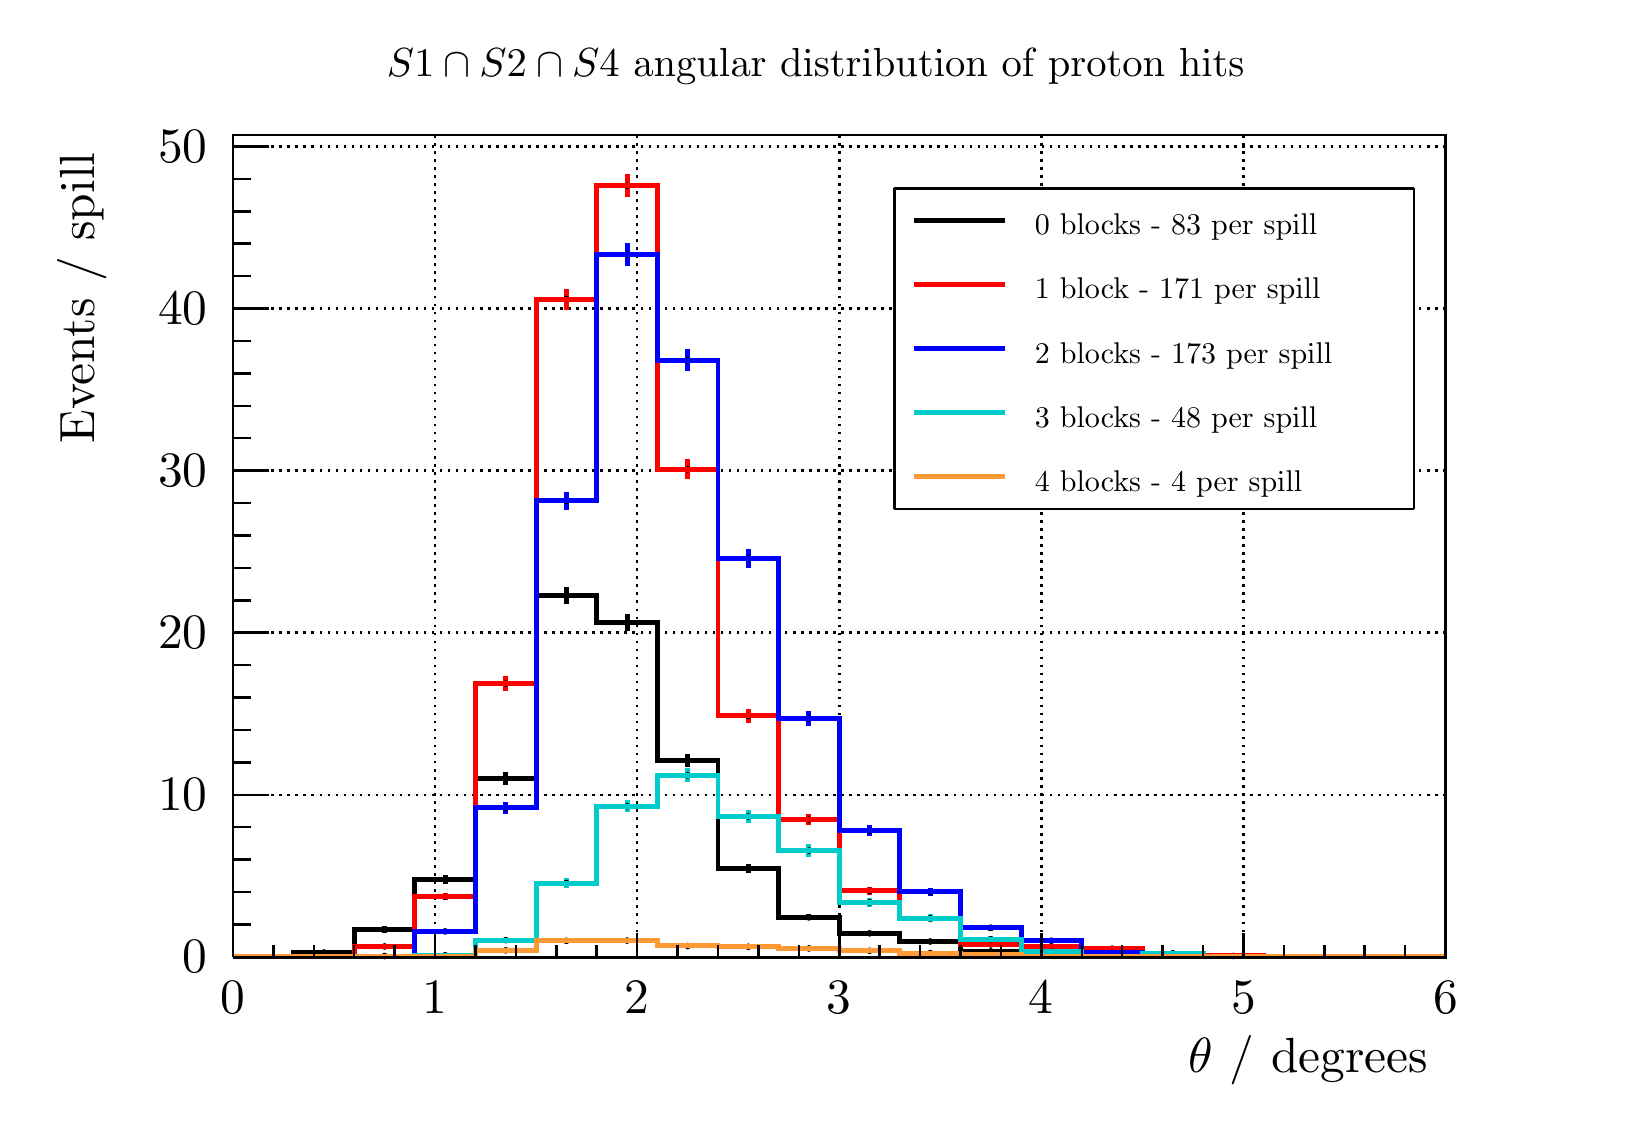
\begin{tikzpicture}
\pgfdeclareplotmark{cross} {
\pgfpathmoveto{\pgfpoint{-0.3\pgfplotmarksize}{\pgfplotmarksize}}
\pgfpathlineto{\pgfpoint{+0.3\pgfplotmarksize}{\pgfplotmarksize}}
\pgfpathlineto{\pgfpoint{+0.3\pgfplotmarksize}{0.3\pgfplotmarksize}}
\pgfpathlineto{\pgfpoint{+1\pgfplotmarksize}{0.3\pgfplotmarksize}}
\pgfpathlineto{\pgfpoint{+1\pgfplotmarksize}{-0.3\pgfplotmarksize}}
\pgfpathlineto{\pgfpoint{+0.3\pgfplotmarksize}{-0.3\pgfplotmarksize}}
\pgfpathlineto{\pgfpoint{+0.3\pgfplotmarksize}{-1.\pgfplotmarksize}}
\pgfpathlineto{\pgfpoint{-0.3\pgfplotmarksize}{-1.\pgfplotmarksize}}
\pgfpathlineto{\pgfpoint{-0.3\pgfplotmarksize}{-0.3\pgfplotmarksize}}
\pgfpathlineto{\pgfpoint{-1.\pgfplotmarksize}{-0.3\pgfplotmarksize}}
\pgfpathlineto{\pgfpoint{-1.\pgfplotmarksize}{0.3\pgfplotmarksize}}
\pgfpathlineto{\pgfpoint{-0.3\pgfplotmarksize}{0.3\pgfplotmarksize}}
\pgfpathclose
\pgfusepathqstroke
}
\pgfdeclareplotmark{cross*} {
\pgfpathmoveto{\pgfpoint{-0.3\pgfplotmarksize}{\pgfplotmarksize}}
\pgfpathlineto{\pgfpoint{+0.3\pgfplotmarksize}{\pgfplotmarksize}}
\pgfpathlineto{\pgfpoint{+0.3\pgfplotmarksize}{0.3\pgfplotmarksize}}
\pgfpathlineto{\pgfpoint{+1\pgfplotmarksize}{0.3\pgfplotmarksize}}
\pgfpathlineto{\pgfpoint{+1\pgfplotmarksize}{-0.3\pgfplotmarksize}}
\pgfpathlineto{\pgfpoint{+0.3\pgfplotmarksize}{-0.3\pgfplotmarksize}}
\pgfpathlineto{\pgfpoint{+0.3\pgfplotmarksize}{-1.\pgfplotmarksize}}
\pgfpathlineto{\pgfpoint{-0.3\pgfplotmarksize}{-1.\pgfplotmarksize}}
\pgfpathlineto{\pgfpoint{-0.3\pgfplotmarksize}{-0.3\pgfplotmarksize}}
\pgfpathlineto{\pgfpoint{-1.\pgfplotmarksize}{-0.3\pgfplotmarksize}}
\pgfpathlineto{\pgfpoint{-1.\pgfplotmarksize}{0.3\pgfplotmarksize}}
\pgfpathlineto{\pgfpoint{-0.3\pgfplotmarksize}{0.3\pgfplotmarksize}}
\pgfpathclose
\pgfusepathqfillstroke
}
\pgfdeclareplotmark{newstar} {
\pgfpathmoveto{\pgfqpoint{0pt}{\pgfplotmarksize}}
\pgfpathlineto{\pgfqpointpolar{44}{0.5\pgfplotmarksize}}
\pgfpathlineto{\pgfqpointpolar{18}{\pgfplotmarksize}}
\pgfpathlineto{\pgfqpointpolar{-20}{0.5\pgfplotmarksize}}
\pgfpathlineto{\pgfqpointpolar{-54}{\pgfplotmarksize}}
\pgfpathlineto{\pgfqpointpolar{-90}{0.5\pgfplotmarksize}}
\pgfpathlineto{\pgfqpointpolar{234}{\pgfplotmarksize}}
\pgfpathlineto{\pgfqpointpolar{198}{0.5\pgfplotmarksize}}
\pgfpathlineto{\pgfqpointpolar{162}{\pgfplotmarksize}}
\pgfpathlineto{\pgfqpointpolar{134}{0.5\pgfplotmarksize}}
\pgfpathclose
\pgfusepathqstroke
}
\pgfdeclareplotmark{newstar*} {
\pgfpathmoveto{\pgfqpoint{0pt}{\pgfplotmarksize}}
\pgfpathlineto{\pgfqpointpolar{44}{0.5\pgfplotmarksize}}
\pgfpathlineto{\pgfqpointpolar{18}{\pgfplotmarksize}}
\pgfpathlineto{\pgfqpointpolar{-20}{0.5\pgfplotmarksize}}
\pgfpathlineto{\pgfqpointpolar{-54}{\pgfplotmarksize}}
\pgfpathlineto{\pgfqpointpolar{-90}{0.5\pgfplotmarksize}}
\pgfpathlineto{\pgfqpointpolar{234}{\pgfplotmarksize}}
\pgfpathlineto{\pgfqpointpolar{198}{0.5\pgfplotmarksize}}
\pgfpathlineto{\pgfqpointpolar{162}{\pgfplotmarksize}}
\pgfpathlineto{\pgfqpointpolar{134}{0.5\pgfplotmarksize}}
\pgfpathclose
\pgfusepathqfillstroke
}
\definecolor{c}{rgb}{1,1,1};
\draw [color=c, fill=c] (0,0) rectangle (20,13.5632);
\draw [color=c, fill=c] (2.6,1.76322) rectangle (18,12.2069);
\definecolor{c}{rgb}{0,0,0};
\draw [c,line width=0.9] (2.6,1.76322) -- (2.6,12.2069) -- (18,12.2069) -- (18,1.76322) -- (2.6,1.76322);
\definecolor{c}{rgb}{1,1,1};
\draw [color=c, fill=c] (2.6,1.76322) rectangle (18,12.2069);
\definecolor{c}{rgb}{0,0,0};
\draw [c,line width=0.9] (2.6,1.76322) -- (2.6,12.2069) -- (18,12.2069) -- (18,1.76322) -- (2.6,1.76322);
\draw [c,line width=0.9] (2.6,1.76322) -- (18,1.76322);
\draw [c,dotted,line width=0.9] (2.6,12.2069) -- (2.6,1.76322);
\draw [c,dotted,line width=0.9] (5.16667,12.2069) -- (5.16667,1.76322);
\draw [c,dotted,line width=0.9] (7.73333,12.2069) -- (7.73333,1.76322);
\draw [c,dotted,line width=0.9] (10.3,12.2069) -- (10.3,1.76322);
\draw [c,dotted,line width=0.9] (12.8667,12.2069) -- (12.8667,1.76322);
\draw [c,dotted,line width=0.9] (15.4333,12.2069) -- (15.4333,1.76322);
\draw [c,dotted,line width=0.9] (18,12.2069) -- (18,1.76322);
\draw [c,line width=0.9] (2.6,1.76322) -- (2.6,12.2069);
\draw [c,dotted,line width=0.9] (18,1.76974) -- (2.6,1.76974);
\draw [c,dotted,line width=0.9] (18,3.82799) -- (2.6,3.82799);
\draw [c,dotted,line width=0.9] (18,5.88624) -- (2.6,5.88624);
\draw [c,dotted,line width=0.9] (18,7.94448) -- (2.6,7.94448);
\draw [c,dotted,line width=0.9] (18,10.0027) -- (2.6,10.0027);
\draw [c,dotted,line width=0.9] (18,12.061) -- (2.6,12.061);
\draw [c,dotted,line width=0.9] (18,1.76974) -- (2.6,1.76974);
\draw [c,dotted,line width=0.9] (18,12.061) -- (2.6,12.061);
\definecolor{c}{rgb}{0,0,0.6};
\draw [c,line width=0.9] (2.6,1.76974) -- (3.37,1.76974) -- (3.37,1.76974) -- (4.14,1.76974) -- (4.14,1.76974) -- (4.91,1.76974) -- (4.91,1.76974) -- (5.68,1.76974) -- (5.68,1.76974) -- (6.45,1.76974) -- (6.45,1.76974) -- (7.22,1.76974) --
 (7.22,1.76974) -- (7.99,1.76974) -- (7.99,1.76974) -- (8.76,1.76974) -- (8.76,1.76974) -- (9.53,1.76974) -- (9.53,1.76974) -- (10.3,1.76974) -- (10.3,1.76974) -- (11.07,1.76974) -- (11.07,1.76974) -- (11.84,1.76974) -- (11.84,1.76974) --
 (12.61,1.76974) -- (12.61,1.76974) -- (13.38,1.76974) -- (13.38,1.76974) -- (14.15,1.76974) -- (14.15,1.76974) -- (14.92,1.76974) -- (14.92,1.76974) -- (15.69,1.76974) -- (15.69,1.76974) -- (16.46,1.76974) -- (16.46,1.76974) -- (17.23,1.76974) --
 (17.23,1.76974) -- (18,1.76974);
\definecolor{c}{rgb}{0,0,0};
\draw [c,line width=0.9] (2.6,1.76322) -- (18,1.76322);
\draw [anchor= east] (18,0.461149) node[scale=1.78699, color=c, rotate=0]{$\theta$ / degrees};
\draw [c,line width=0.9] (2.6,2.07653) -- (2.6,1.76322);
\draw [c,line width=0.9] (3.11333,1.91987) -- (3.11333,1.76322);
\draw [c,line width=0.9] (3.62667,1.91987) -- (3.62667,1.76322);
\draw [c,line width=0.9] (4.14,1.91987) -- (4.14,1.76322);
\draw [c,line width=0.9] (4.65333,1.91987) -- (4.65333,1.76322);
\draw [c,line width=0.9] (5.16667,2.07653) -- (5.16667,1.76322);
\draw [c,line width=0.9] (5.68,1.91987) -- (5.68,1.76322);
\draw [c,line width=0.9] (6.19333,1.91987) -- (6.19333,1.76322);
\draw [c,line width=0.9] (6.70667,1.91987) -- (6.70667,1.76322);
\draw [c,line width=0.9] (7.22,1.91987) -- (7.22,1.76322);
\draw [c,line width=0.9] (7.73333,2.07653) -- (7.73333,1.76322);
\draw [c,line width=0.9] (8.24667,1.91987) -- (8.24667,1.76322);
\draw [c,line width=0.9] (8.76,1.91987) -- (8.76,1.76322);
\draw [c,line width=0.9] (9.27333,1.91987) -- (9.27333,1.76322);
\draw [c,line width=0.9] (9.78667,1.91987) -- (9.78667,1.76322);
\draw [c,line width=0.9] (10.3,2.07653) -- (10.3,1.76322);
\draw [c,line width=0.9] (10.8133,1.91987) -- (10.8133,1.76322);
\draw [c,line width=0.9] (11.3267,1.91987) -- (11.3267,1.76322);
\draw [c,line width=0.9] (11.84,1.91987) -- (11.84,1.76322);
\draw [c,line width=0.9] (12.3533,1.91987) -- (12.3533,1.76322);
\draw [c,line width=0.9] (12.8667,2.07653) -- (12.8667,1.76322);
\draw [c,line width=0.9] (13.38,1.91987) -- (13.38,1.76322);
\draw [c,line width=0.9] (13.8933,1.91987) -- (13.8933,1.76322);
\draw [c,line width=0.9] (14.4067,1.91987) -- (14.4067,1.76322);
\draw [c,line width=0.9] (14.92,1.91987) -- (14.92,1.76322);
\draw [c,line width=0.9] (15.4333,2.07653) -- (15.4333,1.76322);
\draw [c,line width=0.9] (15.9467,1.91987) -- (15.9467,1.76322);
\draw [c,line width=0.9] (16.46,1.91987) -- (16.46,1.76322);
\draw [c,line width=0.9] (16.9733,1.91987) -- (16.9733,1.76322);
\draw [c,line width=0.9] (17.4867,1.91987) -- (17.4867,1.76322);
\draw [c,line width=0.9] (18,2.07653) -- (18,1.76322);
\draw [anchor=base] (2.6,1.04437) node[scale=1.78699, color=c, rotate=0]{0};
\draw [anchor=base] (5.16667,1.04437) node[scale=1.78699, color=c, rotate=0]{1};
\draw [anchor=base] (7.73333,1.04437) node[scale=1.78699, color=c, rotate=0]{2};
\draw [anchor=base] (10.3,1.04437) node[scale=1.78699, color=c, rotate=0]{3};
\draw [anchor=base] (12.8667,1.04437) node[scale=1.78699, color=c, rotate=0]{4};
\draw [anchor=base] (15.4333,1.04437) node[scale=1.78699, color=c, rotate=0]{5};
\draw [anchor=base] (18,1.04437) node[scale=1.78699, color=c, rotate=0]{6};
\draw [c,line width=0.9] (2.6,1.76322) -- (2.6,12.2069);
\draw [anchor= east] (0.68,12.2069) node[scale=1.78699, color=c, rotate=90]{ Events / spill};
\draw [c,line width=0.9] (3.062,1.76974) -- (2.6,1.76974);
\draw [c,line width=0.9] (2.831,2.18139) -- (2.6,2.18139);
\draw [c,line width=0.9] (2.831,2.59304) -- (2.6,2.59304);
\draw [c,line width=0.9] (2.831,3.00469) -- (2.6,3.00469);
\draw [c,line width=0.9] (2.831,3.41634) -- (2.6,3.41634);
\draw [c,line width=0.9] (3.062,3.82799) -- (2.6,3.82799);
\draw [c,line width=0.9] (2.831,4.23964) -- (2.6,4.23964);
\draw [c,line width=0.9] (2.831,4.65129) -- (2.6,4.65129);
\draw [c,line width=0.9] (2.831,5.06294) -- (2.6,5.06294);
\draw [c,line width=0.9] (2.831,5.47459) -- (2.6,5.47459);
\draw [c,line width=0.9] (3.062,5.88624) -- (2.6,5.88624);
\draw [c,line width=0.9] (2.831,6.29789) -- (2.6,6.29789);
\draw [c,line width=0.9] (2.831,6.70953) -- (2.6,6.70953);
\draw [c,line width=0.9] (2.831,7.12118) -- (2.6,7.12118);
\draw [c,line width=0.9] (2.831,7.53283) -- (2.6,7.53283);
\draw [c,line width=0.9] (3.062,7.94448) -- (2.6,7.94448);
\draw [c,line width=0.9] (2.831,8.35613) -- (2.6,8.35613);
\draw [c,line width=0.9] (2.831,8.76778) -- (2.6,8.76778);
\draw [c,line width=0.9] (2.831,9.17943) -- (2.6,9.17943);
\draw [c,line width=0.9] (2.831,9.59108) -- (2.6,9.59108);
\draw [c,line width=0.9] (3.062,10.0027) -- (2.6,10.0027);
\draw [c,line width=0.9] (2.831,10.4144) -- (2.6,10.4144);
\draw [c,line width=0.9] (2.831,10.826) -- (2.6,10.826);
\draw [c,line width=0.9] (2.831,11.2377) -- (2.6,11.2377);
\draw [c,line width=0.9] (2.831,11.6493) -- (2.6,11.6493);
\draw [c,line width=0.9] (3.062,12.061) -- (2.6,12.061);
\draw [c,line width=0.9] (3.062,1.76974) -- (2.6,1.76974);
\draw [c,line width=0.9] (3.062,12.061) -- (2.6,12.061);
\draw [anchor= east] (2.5,1.76974) node[scale=1.78699, color=c, rotate=0]{0};
\draw [anchor= east] (2.5,3.82799) node[scale=1.78699, color=c, rotate=0]{10};
\draw [anchor= east] (2.5,5.88624) node[scale=1.78699, color=c, rotate=0]{20};
\draw [anchor= east] (2.5,7.94448) node[scale=1.78699, color=c, rotate=0]{30};
\draw [anchor= east] (2.5,10.0027) node[scale=1.78699, color=c, rotate=0]{40};
\draw [anchor= east] (2.5,12.061) node[scale=1.78699, color=c, rotate=0]{50};
\draw [c,line width=1.8] (3.755,1.80661) -- (3.755,1.82512);
\draw [c,line width=1.8] (3.755,1.82512) -- (3.755,1.84364);
\foreach \P in {(3.755,1.82512)}{\draw[mark options={color=c,fill=c},mark size=2.402402pt,mark=*,mark size=1pt] plot coordinates {\P};}
\draw [c,line width=1.8] (4.525,2.07739) -- (4.525,2.11837);
\draw [c,line width=1.8] (4.525,2.11837) -- (4.525,2.15935);
\foreach \P in {(4.525,2.11837)}{\draw[mark options={color=c,fill=c},mark size=2.402402pt,mark=*,mark size=1pt] plot coordinates {\P};}
\draw [c,line width=1.8] (5.295,2.68979) -- (5.295,2.75208);
\draw [c,line width=1.8] (5.295,2.75208) -- (5.295,2.81437);
\foreach \P in {(5.295,2.75208)}{\draw[mark options={color=c,fill=c},mark size=2.402402pt,mark=*,mark size=1pt] plot coordinates {\P};}
\draw [c,line width=1.8] (6.065,3.94712) -- (6.065,4.03136);
\draw [c,line width=1.8] (6.065,4.03136) -- (6.065,4.11561);
\foreach \P in {(6.065,4.03136)}{\draw[mark options={color=c,fill=c},mark size=2.402402pt,mark=*,mark size=1pt] plot coordinates {\P};}
\draw [c,line width=1.8] (6.835,6.25543) -- (6.835,6.36302);
\draw [c,line width=1.8] (6.835,6.36302) -- (6.835,6.4706);
\foreach \P in {(6.835,6.36302)}{\draw[mark options={color=c,fill=c},mark size=2.402402pt,mark=*,mark size=1pt] plot coordinates {\P};}
\draw [c,line width=1.8] (7.605,5.91374) -- (7.605,6.01656);
\draw [c,line width=1.8] (7.605,6.01656) -- (7.605,6.11939);
\foreach \P in {(7.605,6.01656)}{\draw[mark options={color=c,fill=c},mark size=2.402402pt,mark=*,mark size=1pt] plot coordinates {\P};}
\draw [c,line width=1.8] (8.375,4.18387) -- (8.375,4.26602);
\draw [c,line width=1.8] (8.375,4.26602) -- (8.375,4.34818);
\foreach \P in {(8.375,4.26602)}{\draw[mark options={color=c,fill=c},mark size=2.402402pt,mark=*,mark size=1pt] plot coordinates {\P};}
\draw [c,line width=1.8] (9.145,2.83028) -- (9.145,2.8869);
\draw [c,line width=1.8] (9.145,2.8869) -- (9.145,2.94353);
\foreach \P in {(9.145,2.8869)}{\draw[mark options={color=c,fill=c},mark size=2.402402pt,mark=*,mark size=1pt] plot coordinates {\P};}
\draw [c,line width=1.8] (9.915,2.2324) -- (9.915,2.27092);
\draw [c,line width=1.8] (9.915,2.27092) -- (9.915,2.30944);
\foreach \P in {(9.915,2.27092)}{\draw[mark options={color=c,fill=c},mark size=2.402402pt,mark=*,mark size=1pt] plot coordinates {\P};}
\draw [c,line width=1.8] (10.685,2.03761) -- (10.685,2.06803);
\draw [c,line width=1.8] (10.685,2.06803) -- (10.685,2.09845);
\foreach \P in {(10.685,2.06803)}{\draw[mark options={color=c,fill=c},mark size=2.402402pt,mark=*,mark size=1pt] plot coordinates {\P};}
\draw [c,line width=1.8] (11.455,1.94017) -- (11.455,1.96434);
\draw [c,line width=1.8] (11.455,1.96434) -- (11.455,1.98852);
\foreach \P in {(11.455,1.96434)}{\draw[mark options={color=c,fill=c},mark size=2.402402pt,mark=*,mark size=1pt] plot coordinates {\P};}
\draw [c,line width=1.8] (12.225,1.82355) -- (12.225,1.83903);
\draw [c,line width=1.8] (12.225,1.83903) -- (12.225,1.85452);
\foreach \P in {(12.225,1.83903)}{\draw[mark options={color=c,fill=c},mark size=2.402402pt,mark=*,mark size=1pt] plot coordinates {\P};}
\draw [c,line width=1.8] (12.995,1.80676) -- (12.995,1.82057);
\draw [c,line width=1.8] (12.995,1.82057) -- (12.995,1.83438);
\foreach \P in {(12.995,1.82057)}{\draw[mark options={color=c,fill=c},mark size=2.402402pt,mark=*,mark size=1pt] plot coordinates {\P};}
\draw [c,line width=1.8] (13.765,1.77723) -- (13.765,1.78745);
\draw [c,line width=1.8] (13.765,1.78745) -- (13.765,1.79768);
\foreach \P in {(13.765,1.78745)}{\draw[mark options={color=c,fill=c},mark size=2.402402pt,mark=*,mark size=1pt] plot coordinates {\P};}
\draw [c,line width=1.8] (14.535,1.78362) -- (14.535,1.79604);
\draw [c,line width=1.8] (14.535,1.79604) -- (14.535,1.80845);
\foreach \P in {(14.535,1.79604)}{\draw[mark options={color=c,fill=c},mark size=2.402402pt,mark=*,mark size=1pt] plot coordinates {\P};}
\draw [c,line width=1.8] (2.6,1.76974) -- (3.37,1.76974) -- (3.37,1.82512) -- (4.14,1.82512) -- (4.14,2.11837) -- (4.91,2.11837) -- (4.91,2.75208) -- (5.68,2.75208) -- (5.68,4.03136) -- (6.45,4.03136) -- (6.45,6.36302) -- (7.22,6.36302) --
 (7.22,6.01656) -- (7.99,6.01656) -- (7.99,4.26602) -- (8.76,4.26602) -- (8.76,2.8869) -- (9.53,2.8869) -- (9.53,2.27092) -- (10.3,2.27092) -- (10.3,2.06803) -- (11.07,2.06803) -- (11.07,1.96434) -- (11.84,1.96434) -- (11.84,1.83903) --
 (12.61,1.83903) -- (12.61,1.82057) -- (13.38,1.82057) -- (13.38,1.78745) -- (14.15,1.78745) -- (14.15,1.79604) -- (14.92,1.79604) -- (14.92,1.76974) -- (15.69,1.76974) -- (15.69,1.76974) -- (16.46,1.76974) -- (16.46,1.76974) -- (17.23,1.76974) --
 (17.23,1.76974) -- (18,1.76974);
\definecolor{c}{rgb}{1,0,0};
\draw [c,line width=1.8] (4.525,1.87963) -- (4.525,1.90177);
\draw [c,line width=1.8] (4.525,1.90177) -- (4.525,1.92392);
\definecolor{c}{rgb}{0,0,0};
\foreach \P in {(4.525,1.90177)}{\draw[mark options={color=c,fill=c},mark size=2.402402pt,mark=*,mark size=1pt] plot coordinates {\P};}
\definecolor{c}{rgb}{1,0,0};
\draw [c,line width=1.8] (5.295,2.48842) -- (5.295,2.53379);
\draw [c,line width=1.8] (5.295,2.53379) -- (5.295,2.57917);
\definecolor{c}{rgb}{0,0,0};
\foreach \P in {(5.295,2.53379)}{\draw[mark options={color=c,fill=c},mark size=2.402402pt,mark=*,mark size=1pt] plot coordinates {\P};}
\definecolor{c}{rgb}{1,0,0};
\draw [c,line width=1.8] (6.065,5.14757) -- (6.065,5.23916);
\draw [c,line width=1.8] (6.065,5.23916) -- (6.065,5.33075);
\definecolor{c}{rgb}{0,0,0};
\foreach \P in {(6.065,5.23916)}{\draw[mark options={color=c,fill=c},mark size=2.402402pt,mark=*,mark size=1pt] plot coordinates {\P};}
\definecolor{c}{rgb}{1,0,0};
\draw [c,line width=1.8] (6.835,9.98824) -- (6.835,10.1229);
\draw [c,line width=1.8] (6.835,10.1229) -- (6.835,10.2575);
\definecolor{c}{rgb}{0,0,0};
\foreach \P in {(6.835,10.1229)}{\draw[mark options={color=c,fill=c},mark size=2.402402pt,mark=*,mark size=1pt] plot coordinates {\P};}
\definecolor{c}{rgb}{1,0,0};
\draw [c,line width=1.8] (7.605,11.4135) -- (7.605,11.5617);
\draw [c,line width=1.8] (7.605,11.5617) -- (7.605,11.7099);
\definecolor{c}{rgb}{0,0,0};
\foreach \P in {(7.605,11.5617)}{\draw[mark options={color=c,fill=c},mark size=2.402402pt,mark=*,mark size=1pt] plot coordinates {\P};}
\definecolor{c}{rgb}{1,0,0};
\draw [c,line width=1.8] (8.375,7.83438) -- (8.375,7.96218);
\draw [c,line width=1.8] (8.375,7.96218) -- (8.375,8.08997);
\definecolor{c}{rgb}{0,0,0};
\foreach \P in {(8.375,7.96218)}{\draw[mark options={color=c,fill=c},mark size=2.402402pt,mark=*,mark size=1pt] plot coordinates {\P};}
\definecolor{c}{rgb}{1,0,0};
\draw [c,line width=1.8] (9.145,4.7362) -- (9.145,4.8288);
\draw [c,line width=1.8] (9.145,4.8288) -- (9.145,4.92141);
\definecolor{c}{rgb}{0,0,0};
\foreach \P in {(9.145,4.8288)}{\draw[mark options={color=c,fill=c},mark size=2.402402pt,mark=*,mark size=1pt] plot coordinates {\P};}
\definecolor{c}{rgb}{1,0,0};
\draw [c,line width=1.8] (9.915,3.44189) -- (9.915,3.51287);
\draw [c,line width=1.8] (9.915,3.51287) -- (9.915,3.58386);
\definecolor{c}{rgb}{0,0,0};
\foreach \P in {(9.915,3.51287)}{\draw[mark options={color=c,fill=c},mark size=2.402402pt,mark=*,mark size=1pt] plot coordinates {\P};}
\definecolor{c}{rgb}{1,0,0};
\draw [c,line width=1.8] (10.685,2.55853) -- (10.685,2.60881);
\draw [c,line width=1.8] (10.685,2.60881) -- (10.685,2.65908);
\definecolor{c}{rgb}{0,0,0};
\foreach \P in {(10.685,2.60881)}{\draw[mark options={color=c,fill=c},mark size=2.402402pt,mark=*,mark size=1pt] plot coordinates {\P};}
\definecolor{c}{rgb}{1,0,0};
\draw [c,line width=1.8] (11.455,2.21208) -- (11.455,2.25177);
\draw [c,line width=1.8] (11.455,2.25177) -- (11.455,2.29147);
\definecolor{c}{rgb}{0,0,0};
\foreach \P in {(11.455,2.25177)}{\draw[mark options={color=c,fill=c},mark size=2.402402pt,mark=*,mark size=1pt] plot coordinates {\P};}
\definecolor{c}{rgb}{1,0,0};
\draw [c,line width=1.8] (12.225,1.90513) -- (12.225,1.92751);
\draw [c,line width=1.8] (12.225,1.92751) -- (12.225,1.94988);
\definecolor{c}{rgb}{0,0,0};
\foreach \P in {(12.225,1.92751)}{\draw[mark options={color=c,fill=c},mark size=2.402402pt,mark=*,mark size=1pt] plot coordinates {\P};}
\definecolor{c}{rgb}{1,0,0};
\draw [c,line width=1.8] (12.995,1.87998) -- (12.995,1.90117);
\draw [c,line width=1.8] (12.995,1.90117) -- (12.995,1.92236);
\definecolor{c}{rgb}{0,0,0};
\foreach \P in {(12.995,1.90117)}{\draw[mark options={color=c,fill=c},mark size=2.402402pt,mark=*,mark size=1pt] plot coordinates {\P};}
\definecolor{c}{rgb}{1,0,0};
\draw [c,line width=1.8] (13.765,1.85362) -- (13.765,1.87401);
\draw [c,line width=1.8] (13.765,1.87401) -- (13.765,1.8944);
\definecolor{c}{rgb}{0,0,0};
\foreach \P in {(13.765,1.87401)}{\draw[mark options={color=c,fill=c},mark size=2.402402pt,mark=*,mark size=1pt] plot coordinates {\P};}
\definecolor{c}{rgb}{1,0,0};
\draw [c,line width=1.8] (14.535,1.78966) -- (14.535,1.80321);
\draw [c,line width=1.8] (14.535,1.80321) -- (14.535,1.81677);
\definecolor{c}{rgb}{0,0,0};
\foreach \P in {(14.535,1.80321)}{\draw[mark options={color=c,fill=c},mark size=2.402402pt,mark=*,mark size=1pt] plot coordinates {\P};}
\definecolor{c}{rgb}{1,0,0};
\draw [c,line width=1.8] (15.305,1.76743) -- (15.305,1.78116);
\draw [c,line width=1.8] (15.305,1.78116) -- (15.305,1.79489);
\definecolor{c}{rgb}{0,0,0};
\foreach \P in {(15.305,1.78116)}{\draw[mark options={color=c,fill=c},mark size=2.402402pt,mark=*,mark size=1pt] plot coordinates {\P};}
\definecolor{c}{rgb}{1,0,0};
\draw [c,line width=1.8] (2.6,1.76974) -- (3.37,1.76974) -- (3.37,1.76974) -- (4.14,1.76974) -- (4.14,1.90177) -- (4.91,1.90177) -- (4.91,2.53379) -- (5.68,2.53379) -- (5.68,5.23916) -- (6.45,5.23916) -- (6.45,10.1229) -- (7.22,10.1229) --
 (7.22,11.5617) -- (7.99,11.5617) -- (7.99,7.96218) -- (8.76,7.96218) -- (8.76,4.8288) -- (9.53,4.8288) -- (9.53,3.51287) -- (10.3,3.51287) -- (10.3,2.60881) -- (11.07,2.60881) -- (11.07,2.25177) -- (11.84,2.25177) -- (11.84,1.92751) --
 (12.61,1.92751) -- (12.61,1.90117) -- (13.38,1.90117) -- (13.38,1.87401) -- (14.15,1.87401) -- (14.15,1.80321) -- (14.92,1.80321) -- (14.92,1.78116) -- (15.69,1.78116) -- (15.69,1.76974) -- (16.46,1.76974) -- (16.46,1.76974) -- (17.23,1.76974) --
 (17.23,1.76974) -- (18,1.76974);
\definecolor{c}{rgb}{0,0,1};
\draw [c,line width=1.8] (4.525,1.76322) -- (4.525,1.77991);
\draw [c,line width=1.8] (4.525,1.77991) -- (4.525,1.7966);
\definecolor{c}{rgb}{0,0,0};
\foreach \P in {(4.525,1.77991)}{\draw[mark options={color=c,fill=c},mark size=2.402402pt,mark=*,mark size=1pt] plot coordinates {\P};}
\definecolor{c}{rgb}{0,0,1};
\draw [c,line width=1.8] (5.295,2.05961) -- (5.295,2.09263);
\draw [c,line width=1.8] (5.295,2.09263) -- (5.295,2.12565);
\definecolor{c}{rgb}{0,0,0};
\foreach \P in {(5.295,2.09263)}{\draw[mark options={color=c,fill=c},mark size=2.402402pt,mark=*,mark size=1pt] plot coordinates {\P};}
\definecolor{c}{rgb}{0,0,1};
\draw [c,line width=1.8] (6.065,3.58922) -- (6.065,3.66036);
\draw [c,line width=1.8] (6.065,3.66036) -- (6.065,3.7315);
\definecolor{c}{rgb}{0,0,0};
\foreach \P in {(6.065,3.66036)}{\draw[mark options={color=c,fill=c},mark size=2.402402pt,mark=*,mark size=1pt] plot coordinates {\P};}
\definecolor{c}{rgb}{0,0,1};
\draw [c,line width=1.8] (6.835,7.44282) -- (6.835,7.56041);
\draw [c,line width=1.8] (6.835,7.56041) -- (6.835,7.678);
\definecolor{c}{rgb}{0,0,0};
\foreach \P in {(6.835,7.56041)}{\draw[mark options={color=c,fill=c},mark size=2.402402pt,mark=*,mark size=1pt] plot coordinates {\P};}
\definecolor{c}{rgb}{0,0,1};
\draw [c,line width=1.8] (7.605,10.5479) -- (7.605,10.6894);
\draw [c,line width=1.8] (7.605,10.6894) -- (7.605,10.8309);
\definecolor{c}{rgb}{0,0,0};
\foreach \P in {(7.605,10.6894)}{\draw[mark options={color=c,fill=c},mark size=2.402402pt,mark=*,mark size=1pt] plot coordinates {\P};}
\definecolor{c}{rgb}{0,0,1};
\draw [c,line width=1.8] (8.375,9.20775) -- (8.375,9.34629);
\draw [c,line width=1.8] (8.375,9.34629) -- (8.375,9.48483);
\definecolor{c}{rgb}{0,0,0};
\foreach \P in {(8.375,9.34629)}{\draw[mark options={color=c,fill=c},mark size=2.402402pt,mark=*,mark size=1pt] plot coordinates {\P};}
\definecolor{c}{rgb}{0,0,1};
\draw [c,line width=1.8] (9.145,6.70824) -- (9.145,6.83094);
\draw [c,line width=1.8] (9.145,6.83094) -- (9.145,6.95365);
\definecolor{c}{rgb}{0,0,0};
\foreach \P in {(9.145,6.83094)}{\draw[mark options={color=c,fill=c},mark size=2.402402pt,mark=*,mark size=1pt] plot coordinates {\P};}
\definecolor{c}{rgb}{0,0,1};
\draw [c,line width=1.8] (9.915,4.7009) -- (9.915,4.79746);
\draw [c,line width=1.8] (9.915,4.79746) -- (9.915,4.89402);
\definecolor{c}{rgb}{0,0,0};
\foreach \P in {(9.915,4.79746)}{\draw[mark options={color=c,fill=c},mark size=2.402402pt,mark=*,mark size=1pt] plot coordinates {\P};}
\definecolor{c}{rgb}{0,0,1};
\draw [c,line width=1.8] (10.685,3.30018) -- (10.685,3.36965);
\draw [c,line width=1.8] (10.685,3.36965) -- (10.685,3.43912);
\definecolor{c}{rgb}{0,0,0};
\foreach \P in {(10.685,3.36965)}{\draw[mark options={color=c,fill=c},mark size=2.402402pt,mark=*,mark size=1pt] plot coordinates {\P};}
\definecolor{c}{rgb}{0,0,1};
\draw [c,line width=1.8] (11.455,2.54232) -- (11.455,2.59381);
\draw [c,line width=1.8] (11.455,2.59381) -- (11.455,2.64531);
\definecolor{c}{rgb}{0,0,0};
\foreach \P in {(11.455,2.59381)}{\draw[mark options={color=c,fill=c},mark size=2.402402pt,mark=*,mark size=1pt] plot coordinates {\P};}
\definecolor{c}{rgb}{0,0,1};
\draw [c,line width=1.8] (12.225,2.10415) -- (12.225,2.13998);
\draw [c,line width=1.8] (12.225,2.13998) -- (12.225,2.1758);
\definecolor{c}{rgb}{0,0,0};
\foreach \P in {(12.225,2.13998)}{\draw[mark options={color=c,fill=c},mark size=2.402402pt,mark=*,mark size=1pt] plot coordinates {\P};}
\definecolor{c}{rgb}{0,0,1};
\draw [c,line width=1.8] (12.995,1.94759) -- (12.995,1.9747);
\draw [c,line width=1.8] (12.995,1.9747) -- (12.995,2.00181);
\definecolor{c}{rgb}{0,0,0};
\foreach \P in {(12.995,1.9747)}{\draw[mark options={color=c,fill=c},mark size=2.402402pt,mark=*,mark size=1pt] plot coordinates {\P};}
\definecolor{c}{rgb}{0,0,1};
\draw [c,line width=1.8] (13.765,1.8042) -- (13.765,1.82296);
\draw [c,line width=1.8] (13.765,1.82296) -- (13.765,1.84173);
\definecolor{c}{rgb}{0,0,0};
\foreach \P in {(13.765,1.82296)}{\draw[mark options={color=c,fill=c},mark size=2.402402pt,mark=*,mark size=1pt] plot coordinates {\P};}
\definecolor{c}{rgb}{0,0,1};
\draw [c,line width=1.8] (14.535,1.79476) -- (14.535,1.8142);
\draw [c,line width=1.8] (14.535,1.8142) -- (14.535,1.83364);
\definecolor{c}{rgb}{0,0,0};
\foreach \P in {(14.535,1.8142)}{\draw[mark options={color=c,fill=c},mark size=2.402402pt,mark=*,mark size=1pt] plot coordinates {\P};}
\definecolor{c}{rgb}{0,0,1};
\draw [c,line width=1.8] (2.6,1.76974) -- (3.37,1.76974) -- (3.37,1.76974) -- (4.14,1.76974) -- (4.14,1.77991) -- (4.91,1.77991) -- (4.91,2.09263) -- (5.68,2.09263) -- (5.68,3.66036) -- (6.45,3.66036) -- (6.45,7.56041) -- (7.22,7.56041) --
 (7.22,10.6894) -- (7.99,10.6894) -- (7.99,9.34629) -- (8.76,9.34629) -- (8.76,6.83094) -- (9.53,6.83094) -- (9.53,4.79746) -- (10.3,4.79746) -- (10.3,3.36965) -- (11.07,3.36965) -- (11.07,2.59381) -- (11.84,2.59381) -- (11.84,2.13998) --
 (12.61,2.13998) -- (12.61,1.9747) -- (13.38,1.9747) -- (13.38,1.82296) -- (14.15,1.82296) -- (14.15,1.8142) -- (14.92,1.8142) -- (14.92,1.76974) -- (15.69,1.76974) -- (15.69,1.76974) -- (16.46,1.76974) -- (16.46,1.76974) -- (17.23,1.76974) --
 (17.23,1.76974) -- (18,1.76974);
\definecolor{c}{rgb}{0,0.8,0.8};
\draw [c,line width=1.8] (5.295,1.77228) -- (5.295,1.79003);
\draw [c,line width=1.8] (5.295,1.79003) -- (5.295,1.80777);
\definecolor{c}{rgb}{0,0,0};
\foreach \P in {(5.295,1.79003)}{\draw[mark options={color=c,fill=c},mark size=2.402402pt,mark=*,mark size=1pt] plot coordinates {\P};}
\definecolor{c}{rgb}{0,0.8,0.8};
\draw [c,line width=1.8] (6.065,1.95127) -- (6.065,1.98182);
\draw [c,line width=1.8] (6.065,1.98182) -- (6.065,2.01237);
\definecolor{c}{rgb}{0,0,0};
\foreach \P in {(6.065,1.98182)}{\draw[mark options={color=c,fill=c},mark size=2.402402pt,mark=*,mark size=1pt] plot coordinates {\P};}
\definecolor{c}{rgb}{0,0.8,0.8};
\draw [c,line width=1.8] (6.835,2.6487) -- (6.835,2.70736);
\draw [c,line width=1.8] (6.835,2.70736) -- (6.835,2.76602);
\definecolor{c}{rgb}{0,0,0};
\foreach \P in {(6.835,2.70736)}{\draw[mark options={color=c,fill=c},mark size=2.402402pt,mark=*,mark size=1pt] plot coordinates {\P};}
\definecolor{c}{rgb}{0,0.8,0.8};
\draw [c,line width=1.8] (7.605,3.60528) -- (7.605,3.68176);
\draw [c,line width=1.8] (7.605,3.68176) -- (7.605,3.75823);
\definecolor{c}{rgb}{0,0,0};
\foreach \P in {(7.605,3.68176)}{\draw[mark options={color=c,fill=c},mark size=2.402402pt,mark=*,mark size=1pt] plot coordinates {\P};}
\definecolor{c}{rgb}{0,0.8,0.8};
\draw [c,line width=1.8] (8.375,3.98782) -- (8.375,4.07498);
\draw [c,line width=1.8] (8.375,4.07498) -- (8.375,4.16215);
\definecolor{c}{rgb}{0,0,0};
\foreach \P in {(8.375,4.07498)}{\draw[mark options={color=c,fill=c},mark size=2.402402pt,mark=*,mark size=1pt] plot coordinates {\P};}
\definecolor{c}{rgb}{0,0.8,0.8};
\draw [c,line width=1.8] (9.145,3.46512) -- (9.145,3.55291);
\draw [c,line width=1.8] (9.145,3.55291) -- (9.145,3.64071);
\definecolor{c}{rgb}{0,0,0};
\foreach \P in {(9.145,3.55291)}{\draw[mark options={color=c,fill=c},mark size=2.402402pt,mark=*,mark size=1pt] plot coordinates {\P};}
\definecolor{c}{rgb}{0,0.8,0.8};
\draw [c,line width=1.8] (9.915,3.03822) -- (9.915,3.11967);
\draw [c,line width=1.8] (9.915,3.11967) -- (9.915,3.20111);
\definecolor{c}{rgb}{0,0,0};
\foreach \P in {(9.915,3.11967)}{\draw[mark options={color=c,fill=c},mark size=2.402402pt,mark=*,mark size=1pt] plot coordinates {\P};}
\definecolor{c}{rgb}{0,0.8,0.8};
\draw [c,line width=1.8] (10.685,2.40584) -- (10.685,2.46168);
\draw [c,line width=1.8] (10.685,2.46168) -- (10.685,2.51752);
\definecolor{c}{rgb}{0,0,0};
\foreach \P in {(10.685,2.46168)}{\draw[mark options={color=c,fill=c},mark size=2.402402pt,mark=*,mark size=1pt] plot coordinates {\P};}
\definecolor{c}{rgb}{0,0.8,0.8};
\draw [c,line width=1.8] (11.455,2.20959) -- (11.455,2.25887);
\draw [c,line width=1.8] (11.455,2.25887) -- (11.455,2.30816);
\definecolor{c}{rgb}{0,0,0};
\foreach \P in {(11.455,2.25887)}{\draw[mark options={color=c,fill=c},mark size=2.402402pt,mark=*,mark size=1pt] plot coordinates {\P};}
\definecolor{c}{rgb}{0,0.8,0.8};
\draw [c,line width=1.8] (12.225,1.95579) -- (12.225,1.99241);
\draw [c,line width=1.8] (12.225,1.99241) -- (12.225,2.02902);
\definecolor{c}{rgb}{0,0,0};
\foreach \P in {(12.225,1.99241)}{\draw[mark options={color=c,fill=c},mark size=2.402402pt,mark=*,mark size=1pt] plot coordinates {\P};}
\definecolor{c}{rgb}{0,0.8,0.8};
\draw [c,line width=1.8] (12.995,1.81125) -- (12.995,1.83513);
\draw [c,line width=1.8] (12.995,1.83513) -- (12.995,1.85902);
\definecolor{c}{rgb}{0,0,0};
\foreach \P in {(12.995,1.83513)}{\draw[mark options={color=c,fill=c},mark size=2.402402pt,mark=*,mark size=1pt] plot coordinates {\P};}
\definecolor{c}{rgb}{0,0.8,0.8};
\draw [c,line width=1.8] (14.535,1.78658) -- (14.535,1.80979);
\draw [c,line width=1.8] (14.535,1.80979) -- (14.535,1.83299);
\definecolor{c}{rgb}{0,0,0};
\foreach \P in {(14.535,1.80979)}{\draw[mark options={color=c,fill=c},mark size=2.402402pt,mark=*,mark size=1pt] plot coordinates {\P};}
\definecolor{c}{rgb}{0,0.8,0.8};
\draw [c,line width=1.8] (2.6,1.76974) -- (3.37,1.76974) -- (3.37,1.76974) -- (4.14,1.76974) -- (4.14,1.76974) -- (4.91,1.76974) -- (4.91,1.79003) -- (5.68,1.79003) -- (5.68,1.98182) -- (6.45,1.98182) -- (6.45,2.70736) -- (7.22,2.70736) --
 (7.22,3.68176) -- (7.99,3.68176) -- (7.99,4.07498) -- (8.76,4.07498) -- (8.76,3.55291) -- (9.53,3.55291) -- (9.53,3.11967) -- (10.3,3.11967) -- (10.3,2.46168) -- (11.07,2.46168) -- (11.07,2.25887) -- (11.84,2.25887) -- (11.84,1.99241) --
 (12.61,1.99241) -- (12.61,1.83513) -- (13.38,1.83513) -- (13.38,1.76974) -- (14.15,1.76974) -- (14.15,1.80979) -- (14.92,1.80979) -- (14.92,1.76974) -- (15.69,1.76974) -- (15.69,1.76974) -- (16.46,1.76974) -- (16.46,1.76974) -- (17.23,1.76974) --
 (17.23,1.76974) -- (18,1.76974);
\definecolor{c}{rgb}{1,0.6,0.2};
\draw [c,line width=1.8] (6.065,1.84606) -- (6.065,1.85249);
\draw [c,line width=1.8] (6.065,1.85249) -- (6.065,1.85892);
\definecolor{c}{rgb}{0,0,0};
\foreach \P in {(6.065,1.85249)}{\draw[mark options={color=c,fill=c},mark size=2.402402pt,mark=*,mark size=1pt] plot coordinates {\P};}
\definecolor{c}{rgb}{1,0.6,0.2};
\draw [c,line width=1.8] (6.835,1.96547) -- (6.835,1.97312);
\draw [c,line width=1.8] (6.835,1.97312) -- (6.835,1.98077);
\definecolor{c}{rgb}{0,0,0};
\foreach \P in {(6.835,1.97312)}{\draw[mark options={color=c,fill=c},mark size=2.402402pt,mark=*,mark size=1pt] plot coordinates {\P};}
\definecolor{c}{rgb}{1,0.6,0.2};
\draw [c,line width=1.8] (7.605,1.96854) -- (7.605,1.97646);
\draw [c,line width=1.8] (7.605,1.97646) -- (7.605,1.98438);
\definecolor{c}{rgb}{0,0,0};
\foreach \P in {(7.605,1.97646)}{\draw[mark options={color=c,fill=c},mark size=2.402402pt,mark=*,mark size=1pt] plot coordinates {\P};}
\definecolor{c}{rgb}{1,0.6,0.2};
\draw [c,line width=1.8] (8.375,1.90074) -- (8.375,1.90807);
\draw [c,line width=1.8] (8.375,1.90807) -- (8.375,1.91539);
\definecolor{c}{rgb}{0,0,0};
\foreach \P in {(8.375,1.90807)}{\draw[mark options={color=c,fill=c},mark size=2.402402pt,mark=*,mark size=1pt] plot coordinates {\P};}
\definecolor{c}{rgb}{1,0.6,0.2};
\draw [c,line width=1.8] (9.145,1.89038) -- (9.145,1.89771);
\draw [c,line width=1.8] (9.145,1.89771) -- (9.145,1.90503);
\definecolor{c}{rgb}{0,0,0};
\foreach \P in {(9.145,1.89771)}{\draw[mark options={color=c,fill=c},mark size=2.402402pt,mark=*,mark size=1pt] plot coordinates {\P};}
\definecolor{c}{rgb}{1,0.6,0.2};
\draw [c,line width=1.8] (9.915,1.8694) -- (9.915,1.8766);
\draw [c,line width=1.8] (9.915,1.8766) -- (9.915,1.88381);
\definecolor{c}{rgb}{0,0,0};
\foreach \P in {(9.915,1.8766)}{\draw[mark options={color=c,fill=c},mark size=2.402402pt,mark=*,mark size=1pt] plot coordinates {\P};}
\definecolor{c}{rgb}{1,0.6,0.2};
\draw [c,line width=1.8] (10.685,1.84033) -- (10.685,1.84725);
\draw [c,line width=1.8] (10.685,1.84725) -- (10.685,1.85417);
\definecolor{c}{rgb}{0,0,0};
\foreach \P in {(10.685,1.84725)}{\draw[mark options={color=c,fill=c},mark size=2.402402pt,mark=*,mark size=1pt] plot coordinates {\P};}
\definecolor{c}{rgb}{1,0.6,0.2};
\draw [c,line width=1.8] (11.455,1.81029) -- (11.455,1.81677);
\draw [c,line width=1.8] (11.455,1.81677) -- (11.455,1.82324);
\definecolor{c}{rgb}{0,0,0};
\foreach \P in {(11.455,1.81677)}{\draw[mark options={color=c,fill=c},mark size=2.402402pt,mark=*,mark size=1pt] plot coordinates {\P};}
\definecolor{c}{rgb}{1,0.6,0.2};
\draw [c,line width=1.8] (12.225,1.79362) -- (12.225,1.80015);
\draw [c,line width=1.8] (12.225,1.80015) -- (12.225,1.80667);
\definecolor{c}{rgb}{0,0,0};
\foreach \P in {(12.225,1.80015)}{\draw[mark options={color=c,fill=c},mark size=2.402402pt,mark=*,mark size=1pt] plot coordinates {\P};}
\definecolor{c}{rgb}{1,0.6,0.2};
\draw [c,line width=1.8] (2.6,1.76974) -- (3.37,1.76974) -- (3.37,1.76974) -- (4.14,1.76974) -- (4.14,1.76974) -- (4.91,1.76974) -- (4.91,1.76974) -- (5.68,1.76974) -- (5.68,1.85249) -- (6.45,1.85249) -- (6.45,1.97312) -- (7.22,1.97312) --
 (7.22,1.97646) -- (7.99,1.97646) -- (7.99,1.90807) -- (8.76,1.90807) -- (8.76,1.89771) -- (9.53,1.89771) -- (9.53,1.8766) -- (10.3,1.8766) -- (10.3,1.84725) -- (11.07,1.84725) -- (11.07,1.81677) -- (11.84,1.81677) -- (11.84,1.80015) --
 (12.61,1.80015) -- (12.61,1.76974) -- (13.38,1.76974) -- (13.38,1.76974) -- (14.15,1.76974) -- (14.15,1.76974) -- (14.92,1.76974) -- (14.92,1.76974) -- (15.69,1.76974) -- (15.69,1.76974) -- (16.46,1.76974) -- (16.46,1.76974) -- (17.23,1.76974) --
 (17.23,1.76974) -- (18,1.76974);
\definecolor{c}{rgb}{0,0,0};
\draw [c,line width=0.9] (2.6,1.76322) -- (18,1.76322);
\draw [c,line width=0.9] (2.6,2.07653) -- (2.6,1.76322);
\draw [c,line width=0.9] (3.11333,1.91987) -- (3.11333,1.76322);
\draw [c,line width=0.9] (3.62667,1.91987) -- (3.62667,1.76322);
\draw [c,line width=0.9] (4.14,1.91987) -- (4.14,1.76322);
\draw [c,line width=0.9] (4.65333,1.91987) -- (4.65333,1.76322);
\draw [c,line width=0.9] (5.16667,2.07653) -- (5.16667,1.76322);
\draw [c,line width=0.9] (5.68,1.91987) -- (5.68,1.76322);
\draw [c,line width=0.9] (6.19333,1.91987) -- (6.19333,1.76322);
\draw [c,line width=0.9] (6.70667,1.91987) -- (6.70667,1.76322);
\draw [c,line width=0.9] (7.22,1.91987) -- (7.22,1.76322);
\draw [c,line width=0.9] (7.73333,2.07653) -- (7.73333,1.76322);
\draw [c,line width=0.9] (8.24667,1.91987) -- (8.24667,1.76322);
\draw [c,line width=0.9] (8.76,1.91987) -- (8.76,1.76322);
\draw [c,line width=0.9] (9.27333,1.91987) -- (9.27333,1.76322);
\draw [c,line width=0.9] (9.78667,1.91987) -- (9.78667,1.76322);
\draw [c,line width=0.9] (10.3,2.07653) -- (10.3,1.76322);
\draw [c,line width=0.9] (10.8133,1.91987) -- (10.8133,1.76322);
\draw [c,line width=0.9] (11.3267,1.91987) -- (11.3267,1.76322);
\draw [c,line width=0.9] (11.84,1.91987) -- (11.84,1.76322);
\draw [c,line width=0.9] (12.3533,1.91987) -- (12.3533,1.76322);
\draw [c,line width=0.9] (12.8667,2.07653) -- (12.8667,1.76322);
\draw [c,line width=0.9] (13.38,1.91987) -- (13.38,1.76322);
\draw [c,line width=0.9] (13.8933,1.91987) -- (13.8933,1.76322);
\draw [c,line width=0.9] (14.4067,1.91987) -- (14.4067,1.76322);
\draw [c,line width=0.9] (14.92,1.91987) -- (14.92,1.76322);
\draw [c,line width=0.9] (15.4333,2.07653) -- (15.4333,1.76322);
\draw [c,line width=0.9] (15.9467,1.91987) -- (15.9467,1.76322);
\draw [c,line width=0.9] (16.46,1.91987) -- (16.46,1.76322);
\draw [c,line width=0.9] (16.9733,1.91987) -- (16.9733,1.76322);
\draw [c,line width=0.9] (17.4867,1.91987) -- (17.4867,1.76322);
\draw [c,line width=0.9] (18,2.07653) -- (18,1.76322);
\draw [c,line width=0.9] (2.6,1.76322) -- (2.6,12.2069);
\draw [c,line width=0.9] (3.062,1.76974) -- (2.6,1.76974);
\draw [c,line width=0.9] (2.831,2.18139) -- (2.6,2.18139);
\draw [c,line width=0.9] (2.831,2.59304) -- (2.6,2.59304);
\draw [c,line width=0.9] (2.831,3.00469) -- (2.6,3.00469);
\draw [c,line width=0.9] (2.831,3.41634) -- (2.6,3.41634);
\draw [c,line width=0.9] (3.062,3.82799) -- (2.6,3.82799);
\draw [c,line width=0.9] (2.831,4.23964) -- (2.6,4.23964);
\draw [c,line width=0.9] (2.831,4.65129) -- (2.6,4.65129);
\draw [c,line width=0.9] (2.831,5.06294) -- (2.6,5.06294);
\draw [c,line width=0.9] (2.831,5.47459) -- (2.6,5.47459);
\draw [c,line width=0.9] (3.062,5.88624) -- (2.6,5.88624);
\draw [c,line width=0.9] (2.831,6.29789) -- (2.6,6.29789);
\draw [c,line width=0.9] (2.831,6.70953) -- (2.6,6.70953);
\draw [c,line width=0.9] (2.831,7.12118) -- (2.6,7.12118);
\draw [c,line width=0.9] (2.831,7.53283) -- (2.6,7.53283);
\draw [c,line width=0.9] (3.062,7.94448) -- (2.6,7.94448);
\draw [c,line width=0.9] (2.831,8.35613) -- (2.6,8.35613);
\draw [c,line width=0.9] (2.831,8.76778) -- (2.6,8.76778);
\draw [c,line width=0.9] (2.831,9.17943) -- (2.6,9.17943);
\draw [c,line width=0.9] (2.831,9.59108) -- (2.6,9.59108);
\draw [c,line width=0.9] (3.062,10.0027) -- (2.6,10.0027);
\draw [c,line width=0.9] (2.831,10.4144) -- (2.6,10.4144);
\draw [c,line width=0.9] (2.831,10.826) -- (2.6,10.826);
\draw [c,line width=0.9] (2.831,11.2377) -- (2.6,11.2377);
\draw [c,line width=0.9] (2.831,11.6493) -- (2.6,11.6493);
\draw [c,line width=0.9] (3.062,12.061) -- (2.6,12.061);
\draw [c,line width=0.9] (3.062,1.76974) -- (2.6,1.76974);
\draw [c,line width=0.9] (3.062,12.061) -- (2.6,12.061);
\draw (10,13.0816) node[scale=1.46788, color=c, rotate=0]{$S1 \cap S2 \cap S4$ angular distribution of proton hits};
\definecolor{c}{rgb}{1,1,1};
\draw [color=c, fill=c] (11,7.45977) rectangle (17.6,11.5287);
\definecolor{c}{rgb}{0,0,0};
\draw [c,line width=0.9] (11,7.45977) -- (17.6,7.45977);
\draw [c,line width=0.9] (17.6,7.45977) -- (17.6,11.5287);
\draw [c,line width=0.9] (17.6,11.5287) -- (11,11.5287);
\draw [c,line width=0.9] (11,11.5287) -- (11,7.45977);
\draw [anchor=base west] (12.65,10.9387) node[scale=1.08496, color=c, rotate=0]{0 blocks - 83 per spill};
\draw [c,line width=1.8] (11.2475,11.1218) -- (12.4025,11.1218);
\draw [anchor=base west] (12.65,10.1249) node[scale=1.08496, color=c, rotate=0]{1 block - 171 per spill};
\definecolor{c}{rgb}{1,0,0};
\draw [c,line width=1.8] (11.2475,10.308) -- (12.4025,10.308);
\definecolor{c}{rgb}{0,0,0};
\draw [anchor=base west] (12.65,9.31115) node[scale=1.08496, color=c, rotate=0]{2 blocks - 173 per spill};
\definecolor{c}{rgb}{0,0,1};
\draw [c,line width=1.8] (11.2475,9.49425) -- (12.4025,9.49425);
\definecolor{c}{rgb}{0,0,0};
\draw [anchor=base west] (12.65,8.49736) node[scale=1.08496, color=c, rotate=0]{3 blocks - 48 per spill};
\definecolor{c}{rgb}{0,0.8,0.8};
\draw [c,line width=1.8] (11.2475,8.68046) -- (12.4025,8.68046);
\definecolor{c}{rgb}{0,0,0};
\draw [anchor=base west] (12.65,7.68356) node[scale=1.08496, color=c, rotate=0]{4 blocks - 4 per spill};
\definecolor{c}{rgb}{1,0.6,0.2};
\draw [c,line width=1.8] (11.2475,7.86667) -- (12.4025,7.86667);
\end{tikzpicture}

	   		\end{adjustbox}
   			\caption{Distribution of hits identified in $S_{4}$ as protons as a function of the number of moderator blocks and the horizontal off-axis angle, as measured from $S_{1}$.}
   		\end{minipage} 
   	
   		%\begin{minipage}[t]{0.48\textwidth}
   		%	\centering
   		%	\includegraphics[width=\textwidth]{files/Figures/piS4Vert}
   		%	\caption{Distribution of hits identified in $S_{4}$ as minimum ionizing particles as a function of the number of moderator blocks and the vertical off-axis angle, as measured from $S_{1}$.}
   		%\end{minipage}
   		%\hspace{0.3cm}
   		%\begin{minipage}[t]{0.48\textwidth}
   		%	\centering
   		%	\includegraphics[width=\textwidth]{files/Figures/proS4Vert}
   		%	\caption{Distribution of hits identified in $S_{4}$ as protons as a function of the number of moderator blocks and the vertical off-axis angle, as measured from $S_{1}$.}
   		%\end{minipage}
   	
	\end{figure}	
        
   	\begin{figure}[ht]
   		\begin{minipage}[t]{0.48\textwidth}
   			\begin{adjustbox}{max totalsize={\textwidth}{.35\textheight}, center}
   				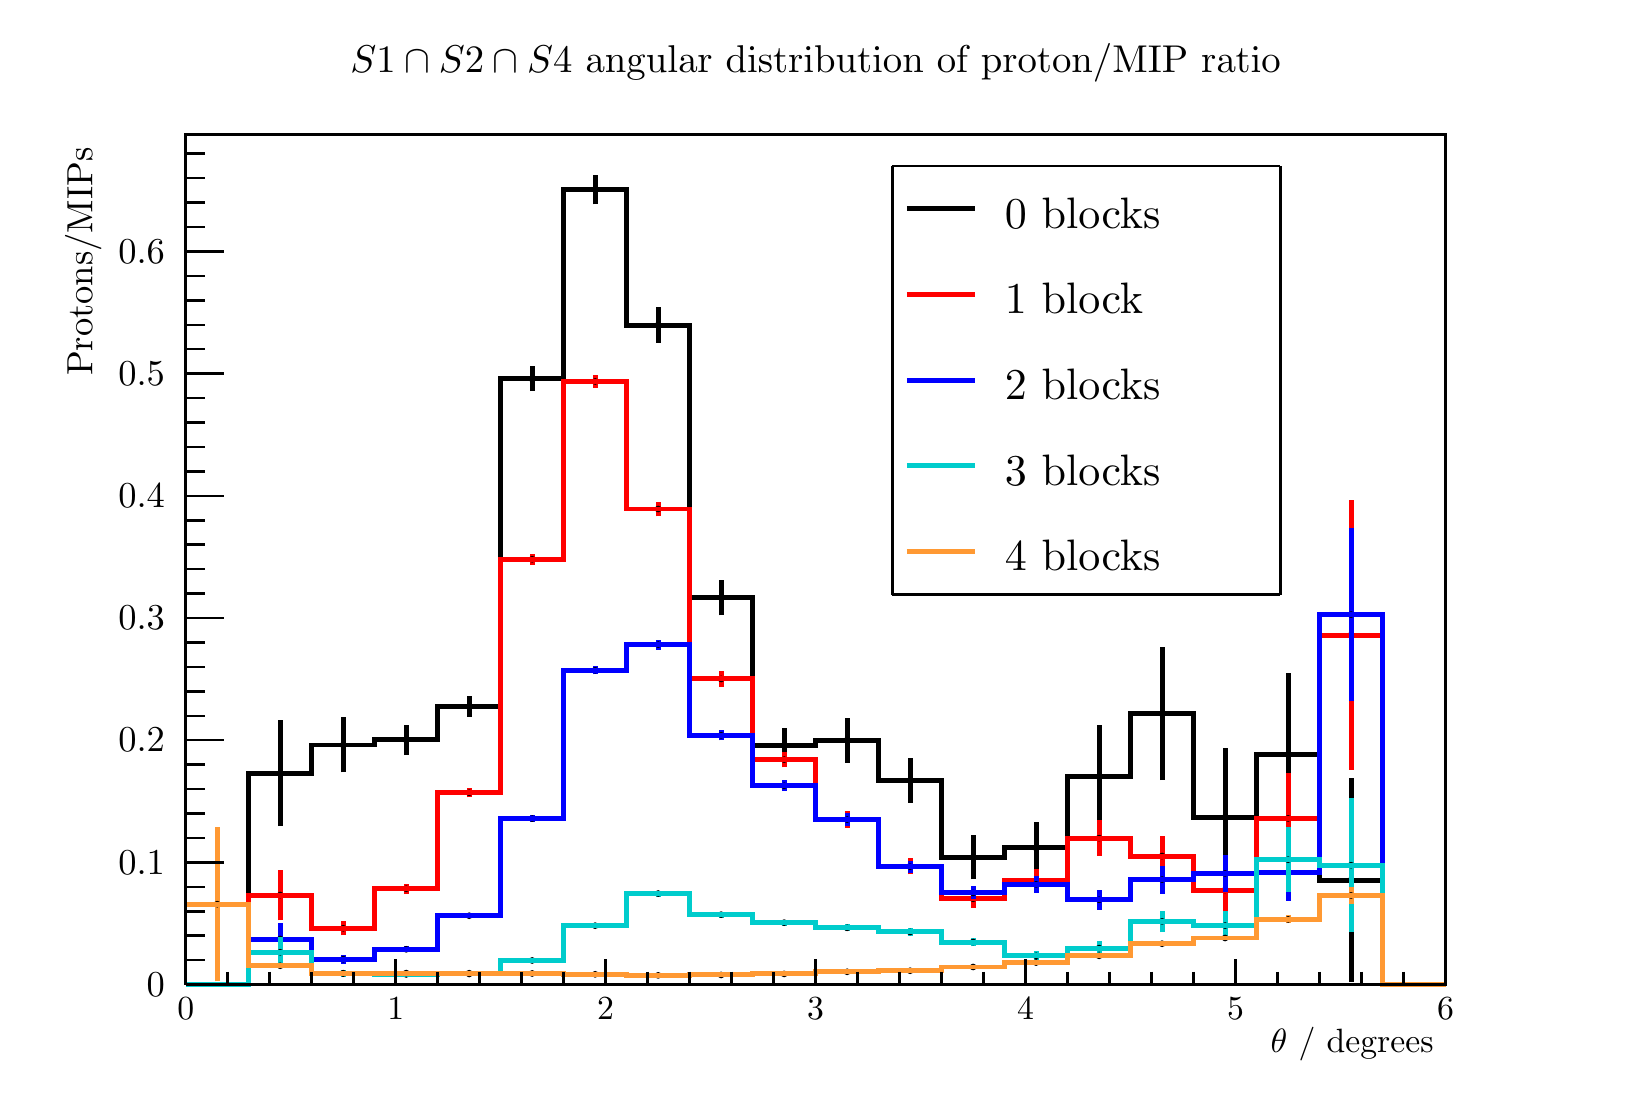
\begin{tikzpicture}
\pgfdeclareplotmark{cross} {
\pgfpathmoveto{\pgfpoint{-0.3\pgfplotmarksize}{\pgfplotmarksize}}
\pgfpathlineto{\pgfpoint{+0.3\pgfplotmarksize}{\pgfplotmarksize}}
\pgfpathlineto{\pgfpoint{+0.3\pgfplotmarksize}{0.3\pgfplotmarksize}}
\pgfpathlineto{\pgfpoint{+1\pgfplotmarksize}{0.3\pgfplotmarksize}}
\pgfpathlineto{\pgfpoint{+1\pgfplotmarksize}{-0.3\pgfplotmarksize}}
\pgfpathlineto{\pgfpoint{+0.3\pgfplotmarksize}{-0.3\pgfplotmarksize}}
\pgfpathlineto{\pgfpoint{+0.3\pgfplotmarksize}{-1.\pgfplotmarksize}}
\pgfpathlineto{\pgfpoint{-0.3\pgfplotmarksize}{-1.\pgfplotmarksize}}
\pgfpathlineto{\pgfpoint{-0.3\pgfplotmarksize}{-0.3\pgfplotmarksize}}
\pgfpathlineto{\pgfpoint{-1.\pgfplotmarksize}{-0.3\pgfplotmarksize}}
\pgfpathlineto{\pgfpoint{-1.\pgfplotmarksize}{0.3\pgfplotmarksize}}
\pgfpathlineto{\pgfpoint{-0.3\pgfplotmarksize}{0.3\pgfplotmarksize}}
\pgfpathclose
\pgfusepathqstroke
}
\pgfdeclareplotmark{cross*} {
\pgfpathmoveto{\pgfpoint{-0.3\pgfplotmarksize}{\pgfplotmarksize}}
\pgfpathlineto{\pgfpoint{+0.3\pgfplotmarksize}{\pgfplotmarksize}}
\pgfpathlineto{\pgfpoint{+0.3\pgfplotmarksize}{0.3\pgfplotmarksize}}
\pgfpathlineto{\pgfpoint{+1\pgfplotmarksize}{0.3\pgfplotmarksize}}
\pgfpathlineto{\pgfpoint{+1\pgfplotmarksize}{-0.3\pgfplotmarksize}}
\pgfpathlineto{\pgfpoint{+0.3\pgfplotmarksize}{-0.3\pgfplotmarksize}}
\pgfpathlineto{\pgfpoint{+0.3\pgfplotmarksize}{-1.\pgfplotmarksize}}
\pgfpathlineto{\pgfpoint{-0.3\pgfplotmarksize}{-1.\pgfplotmarksize}}
\pgfpathlineto{\pgfpoint{-0.3\pgfplotmarksize}{-0.3\pgfplotmarksize}}
\pgfpathlineto{\pgfpoint{-1.\pgfplotmarksize}{-0.3\pgfplotmarksize}}
\pgfpathlineto{\pgfpoint{-1.\pgfplotmarksize}{0.3\pgfplotmarksize}}
\pgfpathlineto{\pgfpoint{-0.3\pgfplotmarksize}{0.3\pgfplotmarksize}}
\pgfpathclose
\pgfusepathqfillstroke
}
\pgfdeclareplotmark{newstar} {
\pgfpathmoveto{\pgfqpoint{0pt}{\pgfplotmarksize}}
\pgfpathlineto{\pgfqpointpolar{44}{0.5\pgfplotmarksize}}
\pgfpathlineto{\pgfqpointpolar{18}{\pgfplotmarksize}}
\pgfpathlineto{\pgfqpointpolar{-20}{0.5\pgfplotmarksize}}
\pgfpathlineto{\pgfqpointpolar{-54}{\pgfplotmarksize}}
\pgfpathlineto{\pgfqpointpolar{-90}{0.5\pgfplotmarksize}}
\pgfpathlineto{\pgfqpointpolar{234}{\pgfplotmarksize}}
\pgfpathlineto{\pgfqpointpolar{198}{0.5\pgfplotmarksize}}
\pgfpathlineto{\pgfqpointpolar{162}{\pgfplotmarksize}}
\pgfpathlineto{\pgfqpointpolar{134}{0.5\pgfplotmarksize}}
\pgfpathclose
\pgfusepathqstroke
}
\pgfdeclareplotmark{newstar*} {
\pgfpathmoveto{\pgfqpoint{0pt}{\pgfplotmarksize}}
\pgfpathlineto{\pgfqpointpolar{44}{0.5\pgfplotmarksize}}
\pgfpathlineto{\pgfqpointpolar{18}{\pgfplotmarksize}}
\pgfpathlineto{\pgfqpointpolar{-20}{0.5\pgfplotmarksize}}
\pgfpathlineto{\pgfqpointpolar{-54}{\pgfplotmarksize}}
\pgfpathlineto{\pgfqpointpolar{-90}{0.5\pgfplotmarksize}}
\pgfpathlineto{\pgfqpointpolar{234}{\pgfplotmarksize}}
\pgfpathlineto{\pgfqpointpolar{198}{0.5\pgfplotmarksize}}
\pgfpathlineto{\pgfqpointpolar{162}{\pgfplotmarksize}}
\pgfpathlineto{\pgfqpointpolar{134}{0.5\pgfplotmarksize}}
\pgfpathclose
\pgfusepathqfillstroke
}
\definecolor{c}{rgb}{1,1,1};
\draw [color=c, fill=c] (0,0) rectangle (20,13.4957);
\draw [color=c, fill=c] (2,1.34957) rectangle (18,12.1461);
\definecolor{c}{rgb}{0,0,0};
\draw [c,line width=0.9] (2,1.34957) -- (2,12.1461) -- (18,12.1461) -- (18,1.34957) -- (2,1.34957);
\definecolor{c}{rgb}{1,1,1};
\draw [color=c, fill=c] (2,1.34957) rectangle (18,12.1461);
\definecolor{c}{rgb}{0,0,0};
\draw [c,line width=0.9] (2,1.34957) -- (2,12.1461) -- (18,12.1461) -- (18,1.34957) -- (2,1.34957);
\definecolor{c}{rgb}{0,0,0.6};
\draw [c,line width=0.9] (2,1.34957) -- (2.8,1.34957) -- (2.8,1.34957) -- (3.6,1.34957) -- (3.6,1.34957) -- (4.4,1.34957) -- (4.4,1.34957) -- (5.2,1.34957) -- (5.2,1.34957) -- (6,1.34957) -- (6,1.34957) -- (6.8,1.34957) -- (6.8,1.34957) --
 (7.6,1.34957) -- (7.6,1.34957) -- (8.4,1.34957) -- (8.4,1.34957) -- (9.2,1.34957) -- (9.2,1.34957) -- (10,1.34957) -- (10,1.34957) -- (10.8,1.34957) -- (10.8,1.34957) -- (11.6,1.34957) -- (11.6,1.34957) -- (12.4,1.34957) -- (12.4,1.34957) --
 (13.2,1.34957) -- (13.2,1.34957) -- (14,1.34957) -- (14,1.34957) -- (14.8,1.34957) -- (14.8,1.34957) -- (15.6,1.34957) -- (15.6,1.34957) -- (16.4,1.34957) -- (16.4,1.34957) -- (17.2,1.34957) -- (17.2,1.34957) -- (18,1.34957);
\definecolor{c}{rgb}{0,0,0};
\draw [c,line width=0.9] (2,1.34957) -- (18,1.34957);
\draw [c,line width=0.9] (2,1.67347) -- (2,1.34957);
\draw [c,line width=0.9] (2.53333,1.51152) -- (2.53333,1.34957);
\draw [c,line width=0.9] (3.06667,1.51152) -- (3.06667,1.34957);
\draw [c,line width=0.9] (3.6,1.51152) -- (3.6,1.34957);
\draw [c,line width=0.9] (4.13333,1.51152) -- (4.13333,1.34957);
\draw [c,line width=0.9] (4.66667,1.67347) -- (4.66667,1.34957);
\draw [c,line width=0.9] (5.2,1.51152) -- (5.2,1.34957);
\draw [c,line width=0.9] (5.73333,1.51152) -- (5.73333,1.34957);
\draw [c,line width=0.9] (6.26667,1.51152) -- (6.26667,1.34957);
\draw [c,line width=0.9] (6.8,1.51152) -- (6.8,1.34957);
\draw [c,line width=0.9] (7.33333,1.67347) -- (7.33333,1.34957);
\draw [c,line width=0.9] (7.86667,1.51152) -- (7.86667,1.34957);
\draw [c,line width=0.9] (8.4,1.51152) -- (8.4,1.34957);
\draw [c,line width=0.9] (8.93333,1.51152) -- (8.93333,1.34957);
\draw [c,line width=0.9] (9.46667,1.51152) -- (9.46667,1.34957);
\draw [c,line width=0.9] (10,1.67347) -- (10,1.34957);
\draw [c,line width=0.9] (10.5333,1.51152) -- (10.5333,1.34957);
\draw [c,line width=0.9] (11.0667,1.51152) -- (11.0667,1.34957);
\draw [c,line width=0.9] (11.6,1.51152) -- (11.6,1.34957);
\draw [c,line width=0.9] (12.1333,1.51152) -- (12.1333,1.34957);
\draw [c,line width=0.9] (12.6667,1.67347) -- (12.6667,1.34957);
\draw [c,line width=0.9] (13.2,1.51152) -- (13.2,1.34957);
\draw [c,line width=0.9] (13.7333,1.51152) -- (13.7333,1.34957);
\draw [c,line width=0.9] (14.2667,1.51152) -- (14.2667,1.34957);
\draw [c,line width=0.9] (14.8,1.51152) -- (14.8,1.34957);
\draw [c,line width=0.9] (15.3333,1.67347) -- (15.3333,1.34957);
\draw [c,line width=0.9] (15.8667,1.51152) -- (15.8667,1.34957);
\draw [c,line width=0.9] (16.4,1.51152) -- (16.4,1.34957);
\draw [c,line width=0.9] (16.9333,1.51152) -- (16.9333,1.34957);
\draw [c,line width=0.9] (17.4667,1.51152) -- (17.4667,1.34957);
\draw [c,line width=0.9] (18,1.67347) -- (18,1.34957);
\draw [anchor=base] (2,0.904212) node[scale=1.21821, color=c, rotate=0]{0};
\draw [anchor=base] (4.66667,0.904212) node[scale=1.21821, color=c, rotate=0]{1};
\draw [anchor=base] (7.33333,0.904212) node[scale=1.21821, color=c, rotate=0]{2};
\draw [anchor=base] (10,0.904212) node[scale=1.21821, color=c, rotate=0]{3};
\draw [anchor=base] (12.6667,0.904212) node[scale=1.21821, color=c, rotate=0]{4};
\draw [anchor=base] (15.3333,0.904212) node[scale=1.21821, color=c, rotate=0]{5};
\draw [anchor=base] (18,0.904212) node[scale=1.21821, color=c, rotate=0]{6};
\draw [anchor= east] (18,0.593811) node[scale=1.21821, color=c, rotate=0]{$\theta$ / degrees};
\draw [c,line width=0.9] (2,1.34957) -- (2,12.1461);
\draw [c,line width=0.9] (2.48,1.34957) -- (2,1.34957);
\draw [c,line width=0.9] (2.24,1.65993) -- (2,1.65993);
\draw [c,line width=0.9] (2.24,1.97029) -- (2,1.97029);
\draw [c,line width=0.9] (2.24,2.28066) -- (2,2.28066);
\draw [c,line width=0.9] (2.24,2.59102) -- (2,2.59102);
\draw [c,line width=0.9] (2.48,2.90138) -- (2,2.90138);
\draw [c,line width=0.9] (2.24,3.21174) -- (2,3.21174);
\draw [c,line width=0.9] (2.24,3.5221) -- (2,3.5221);
\draw [c,line width=0.9] (2.24,3.83247) -- (2,3.83247);
\draw [c,line width=0.9] (2.24,4.14283) -- (2,4.14283);
\draw [c,line width=0.9] (2.48,4.45319) -- (2,4.45319);
\draw [c,line width=0.9] (2.24,4.76355) -- (2,4.76355);
\draw [c,line width=0.9] (2.24,5.07391) -- (2,5.07391);
\draw [c,line width=0.9] (2.24,5.38428) -- (2,5.38428);
\draw [c,line width=0.9] (2.24,5.69464) -- (2,5.69464);
\draw [c,line width=0.9] (2.48,6.005) -- (2,6.005);
\draw [c,line width=0.9] (2.24,6.31536) -- (2,6.31536);
\draw [c,line width=0.9] (2.24,6.62572) -- (2,6.62572);
\draw [c,line width=0.9] (2.24,6.93609) -- (2,6.93609);
\draw [c,line width=0.9] (2.24,7.24645) -- (2,7.24645);
\draw [c,line width=0.9] (2.48,7.55681) -- (2,7.55681);
\draw [c,line width=0.9] (2.24,7.86717) -- (2,7.86717);
\draw [c,line width=0.9] (2.24,8.17753) -- (2,8.17753);
\draw [c,line width=0.9] (2.24,8.4879) -- (2,8.4879);
\draw [c,line width=0.9] (2.24,8.79826) -- (2,8.79826);
\draw [c,line width=0.9] (2.48,9.10862) -- (2,9.10862);
\draw [c,line width=0.9] (2.24,9.41898) -- (2,9.41898);
\draw [c,line width=0.9] (2.24,9.72934) -- (2,9.72934);
\draw [c,line width=0.9] (2.24,10.0397) -- (2,10.0397);
\draw [c,line width=0.9] (2.24,10.3501) -- (2,10.3501);
\draw [c,line width=0.9] (2.48,10.6604) -- (2,10.6604);
\draw [c,line width=0.9] (2.48,10.6604) -- (2,10.6604);
\draw [c,line width=0.9] (2.24,10.9708) -- (2,10.9708);
\draw [c,line width=0.9] (2.24,11.2812) -- (2,11.2812);
\draw [c,line width=0.9] (2.24,11.5915) -- (2,11.5915);
\draw [c,line width=0.9] (2.24,11.9019) -- (2,11.9019);
\draw [anchor= east] (1.9,1.34957) node[scale=1.31821, color=c, rotate=0]{0};
\draw [anchor= east] (1.9,2.90138) node[scale=1.31821, color=c, rotate=0]{0.1};
\draw [anchor= east] (1.9,4.45319) node[scale=1.31821, color=c, rotate=0]{0.2};
\draw [anchor= east] (1.9,6.005) node[scale=1.31821, color=c, rotate=0]{0.3};
\draw [anchor= east] (1.9,7.55681) node[scale=1.31821, color=c, rotate=0]{0.4};
\draw [anchor= east] (1.9,9.10862) node[scale=1.31821, color=c, rotate=0]{0.5};
\draw [anchor= east] (1.9,10.6604) node[scale=1.31821, color=c, rotate=0]{0.6};
\draw [anchor= east] (0.698281,12.1461) node[scale=1.31821, color=c, rotate=90]{ Protons/MIPs};
\draw [c,line width=1.8] (3.2,3.36179) -- (3.2,4.03295);
\draw [c,line width=1.8] (3.2,4.03295) -- (3.2,4.70411);
\foreach \P in {(3.2,4.03295)}{\draw[mark options={color=c,fill=c},mark size=2.402402pt,mark=*,mark size=1pt] plot coordinates {\P};}
\draw [c,line width=1.8] (4,4.04344) -- (4,4.39272);
\draw [c,line width=1.8] (4,4.39272) -- (4,4.74201);
\foreach \P in {(4,4.39272)}{\draw[mark options={color=c,fill=c},mark size=2.402402pt,mark=*,mark size=1pt] plot coordinates {\P};}
\draw [c,line width=1.8] (4.8,4.26335) -- (4.8,4.4571);
\draw [c,line width=1.8] (4.8,4.4571) -- (4.8,4.65085);
\foreach \P in {(4.8,4.4571)}{\draw[mark options={color=c,fill=c},mark size=2.402402pt,mark=*,mark size=1pt] plot coordinates {\P};}
\draw [c,line width=1.8] (5.6,4.75199) -- (5.6,4.88067);
\draw [c,line width=1.8] (5.6,4.88067) -- (5.6,5.00935);
\foreach \P in {(5.6,4.88067)}{\draw[mark options={color=c,fill=c},mark size=2.402402pt,mark=*,mark size=1pt] plot coordinates {\P};}
\draw [c,line width=1.8] (6.4,8.88632) -- (6.4,9.04345);
\draw [c,line width=1.8] (6.4,9.04345) -- (6.4,9.20059);
\foreach \P in {(6.4,9.04345)}{\draw[mark options={color=c,fill=c},mark size=2.402402pt,mark=*,mark size=1pt] plot coordinates {\P};}
\draw [c,line width=1.8] (7.2,11.2585) -- (7.2,11.4452);
\draw [c,line width=1.8] (7.2,11.4452) -- (7.2,11.632);
\foreach \P in {(7.2,11.4452)}{\draw[mark options={color=c,fill=c},mark size=2.402402pt,mark=*,mark size=1pt] plot coordinates {\P};}
\draw [c,line width=1.8] (8,9.50176) -- (8,9.72619);
\draw [c,line width=1.8] (8,9.72619) -- (8,9.95062);
\foreach \P in {(8,9.72619)}{\draw[mark options={color=c,fill=c},mark size=2.402402pt,mark=*,mark size=1pt] plot coordinates {\P};}
\draw [c,line width=1.8] (8.8,6.03742) -- (8.8,6.26476);
\draw [c,line width=1.8] (8.8,6.26476) -- (8.8,6.49209);
\foreach \P in {(8.8,6.26476)}{\draw[mark options={color=c,fill=c},mark size=2.402402pt,mark=*,mark size=1pt] plot coordinates {\P};}
\draw [c,line width=1.8] (9.6,4.17067) -- (9.6,4.38778);
\draw [c,line width=1.8] (9.6,4.38778) -- (9.6,4.60489);
\foreach \P in {(9.6,4.38778)}{\draw[mark options={color=c,fill=c},mark size=2.402402pt,mark=*,mark size=1pt] plot coordinates {\P};}
\draw [c,line width=1.8] (10.4,4.16928) -- (10.4,4.45413);
\draw [c,line width=1.8] (10.4,4.45413) -- (10.4,4.73898);
\foreach \P in {(10.4,4.45413)}{\draw[mark options={color=c,fill=c},mark size=2.402402pt,mark=*,mark size=1pt] plot coordinates {\P};}
\draw [c,line width=1.8] (11.2,3.65873) -- (11.2,3.9425);
\draw [c,line width=1.8] (11.2,3.9425) -- (11.2,4.22627);
\foreach \P in {(11.2,3.9425)}{\draw[mark options={color=c,fill=c},mark size=2.402402pt,mark=*,mark size=1pt] plot coordinates {\P};}
\draw [c,line width=1.8] (12,2.68697) -- (12,2.96624);
\draw [c,line width=1.8] (12,2.96624) -- (12,3.24551);
\foreach \P in {(12,2.96624)}{\draw[mark options={color=c,fill=c},mark size=2.402402pt,mark=*,mark size=1pt] plot coordinates {\P};}
\draw [c,line width=1.8] (12.8,2.75278) -- (12.8,3.08523);
\draw [c,line width=1.8] (12.8,3.08523) -- (12.8,3.41768);
\foreach \P in {(12.8,3.08523)}{\draw[mark options={color=c,fill=c},mark size=2.402402pt,mark=*,mark size=1pt] plot coordinates {\P};}
\draw [c,line width=1.8] (13.6,3.34399) -- (13.6,3.99224);
\draw [c,line width=1.8] (13.6,3.99224) -- (13.6,4.6405);
\foreach \P in {(13.6,3.99224)}{\draw[mark options={color=c,fill=c},mark size=2.402402pt,mark=*,mark size=1pt] plot coordinates {\P};}
\draw [c,line width=1.8] (14.4,3.94704) -- (14.4,4.78987);
\draw [c,line width=1.8] (14.4,4.78987) -- (14.4,5.63269);
\foreach \P in {(14.4,4.78987)}{\draw[mark options={color=c,fill=c},mark size=2.402402pt,mark=*,mark size=1pt] plot coordinates {\P};}
\draw [c,line width=1.8] (15.2,2.5973) -- (15.2,3.4749);
\draw [c,line width=1.8] (15.2,3.4749) -- (15.2,4.3525);
\foreach \P in {(15.2,3.4749)}{\draw[mark options={color=c,fill=c},mark size=2.402402pt,mark=*,mark size=1pt] plot coordinates {\P};}
\draw [c,line width=1.8] (16,3.23371) -- (16,4.27199);
\draw [c,line width=1.8] (16,4.27199) -- (16,5.31028);
\foreach \P in {(16,4.27199)}{\draw[mark options={color=c,fill=c},mark size=2.402402pt,mark=*,mark size=1pt] plot coordinates {\P};}
\draw [c,line width=1.8] (16.8,1.38433) -- (16.8,2.67746);
\draw [c,line width=1.8] (16.8,2.67746) -- (16.8,3.97058);
\foreach \P in {(16.8,2.67746)}{\draw[mark options={color=c,fill=c},mark size=2.402402pt,mark=*,mark size=1pt] plot coordinates {\P};}
\draw [c,line width=1.8] (2,1.34957) -- (2.8,1.34957) -- (2.8,4.03295) -- (3.6,4.03295) -- (3.6,4.39272) -- (4.4,4.39272) -- (4.4,4.4571) -- (5.2,4.4571) -- (5.2,4.88067) -- (6,4.88067) -- (6,9.04345) -- (6.8,9.04345) -- (6.8,11.4452) --
 (7.6,11.4452) -- (7.6,9.72619) -- (8.4,9.72619) -- (8.4,6.26476) -- (9.2,6.26476) -- (9.2,4.38778) -- (10,4.38778) -- (10,4.45413) -- (10.8,4.45413) -- (10.8,3.9425) -- (11.6,3.9425) -- (11.6,2.96624) -- (12.4,2.96624) -- (12.4,3.08523) --
 (13.2,3.08523) -- (13.2,3.99224) -- (14,3.99224) -- (14,4.78987) -- (14.8,4.78987) -- (14.8,3.4749) -- (15.6,3.4749) -- (15.6,4.27199) -- (16.4,4.27199) -- (16.4,2.67746) -- (17.2,2.67746) -- (17.2,1.34957) -- (18,1.34957);
\definecolor{c}{rgb}{1,0,0};
\draw [c,line width=1.8] (3.2,2.16442) -- (3.2,2.48721);
\draw [c,line width=1.8] (3.2,2.48721) -- (3.2,2.80999);
\definecolor{c}{rgb}{0,0,0};
\foreach \P in {(3.2,2.48721)}{\draw[mark options={color=c,fill=c},mark size=2.402402pt,mark=*,mark size=1pt] plot coordinates {\P};}
\definecolor{c}{rgb}{1,0,0};
\draw [c,line width=1.8] (4,1.97443) -- (4,2.06512);
\draw [c,line width=1.8] (4,2.06512) -- (4,2.15581);
\definecolor{c}{rgb}{0,0,0};
\foreach \P in {(4,2.06512)}{\draw[mark options={color=c,fill=c},mark size=2.402402pt,mark=*,mark size=1pt] plot coordinates {\P};}
\definecolor{c}{rgb}{1,0,0};
\draw [c,line width=1.8] (4.8,2.50015) -- (4.8,2.56691);
\draw [c,line width=1.8] (4.8,2.56691) -- (4.8,2.63366);
\definecolor{c}{rgb}{0,0,0};
\foreach \P in {(4.8,2.56691)}{\draw[mark options={color=c,fill=c},mark size=2.402402pt,mark=*,mark size=1pt] plot coordinates {\P};}
\definecolor{c}{rgb}{1,0,0};
\draw [c,line width=1.8] (5.6,3.72718) -- (5.6,3.78634);
\draw [c,line width=1.8] (5.6,3.78634) -- (5.6,3.84549);
\definecolor{c}{rgb}{0,0,0};
\foreach \P in {(5.6,3.78634)}{\draw[mark options={color=c,fill=c},mark size=2.402402pt,mark=*,mark size=1pt] plot coordinates {\P};}
\definecolor{c}{rgb}{1,0,0};
\draw [c,line width=1.8] (6.4,6.68083) -- (6.4,6.75163);
\draw [c,line width=1.8] (6.4,6.75163) -- (6.4,6.82242);
\definecolor{c}{rgb}{0,0,0};
\foreach \P in {(6.4,6.75163)}{\draw[mark options={color=c,fill=c},mark size=2.402402pt,mark=*,mark size=1pt] plot coordinates {\P};}
\definecolor{c}{rgb}{1,0,0};
\draw [c,line width=1.8] (7.2,8.92748) -- (7.2,9.00968);
\draw [c,line width=1.8] (7.2,9.00968) -- (7.2,9.09189);
\definecolor{c}{rgb}{0,0,0};
\foreach \P in {(7.2,9.00968)}{\draw[mark options={color=c,fill=c},mark size=2.402402pt,mark=*,mark size=1pt] plot coordinates {\P};}
\definecolor{c}{rgb}{1,0,0};
\draw [c,line width=1.8] (8,7.29635) -- (8,7.38984);
\draw [c,line width=1.8] (8,7.38984) -- (8,7.48334);
\definecolor{c}{rgb}{0,0,0};
\foreach \P in {(8,7.38984)}{\draw[mark options={color=c,fill=c},mark size=2.402402pt,mark=*,mark size=1pt] plot coordinates {\P};}
\definecolor{c}{rgb}{1,0,0};
\draw [c,line width=1.8] (8.8,5.13448) -- (8.8,5.23128);
\draw [c,line width=1.8] (8.8,5.23128) -- (8.8,5.32808);
\definecolor{c}{rgb}{0,0,0};
\foreach \P in {(8.8,5.23128)}{\draw[mark options={color=c,fill=c},mark size=2.402402pt,mark=*,mark size=1pt] plot coordinates {\P};}
\definecolor{c}{rgb}{1,0,0};
\draw [c,line width=1.8] (9.6,4.10846) -- (9.6,4.20712);
\draw [c,line width=1.8] (9.6,4.20712) -- (9.6,4.30577);
\definecolor{c}{rgb}{0,0,0};
\foreach \P in {(9.6,4.20712)}{\draw[mark options={color=c,fill=c},mark size=2.402402pt,mark=*,mark size=1pt] plot coordinates {\P};}
\definecolor{c}{rgb}{1,0,0};
\draw [c,line width=1.8] (10.4,3.34079) -- (10.4,3.44744);
\draw [c,line width=1.8] (10.4,3.44744) -- (10.4,3.55409);
\definecolor{c}{rgb}{0,0,0};
\foreach \P in {(10.4,3.44744)}{\draw[mark options={color=c,fill=c},mark size=2.402402pt,mark=*,mark size=1pt] plot coordinates {\P};}
\definecolor{c}{rgb}{1,0,0};
\draw [c,line width=1.8] (11.2,2.75027) -- (11.2,2.85305);
\draw [c,line width=1.8] (11.2,2.85305) -- (11.2,2.95583);
\definecolor{c}{rgb}{0,0,0};
\foreach \P in {(11.2,2.85305)}{\draw[mark options={color=c,fill=c},mark size=2.402402pt,mark=*,mark size=1pt] plot coordinates {\P};}
\definecolor{c}{rgb}{1,0,0};
\draw [c,line width=1.8] (12,2.32887) -- (12,2.43947);
\draw [c,line width=1.8] (12,2.43947) -- (12,2.55008);
\definecolor{c}{rgb}{0,0,0};
\foreach \P in {(12,2.43947)}{\draw[mark options={color=c,fill=c},mark size=2.402402pt,mark=*,mark size=1pt] plot coordinates {\P};}
\definecolor{c}{rgb}{1,0,0};
\draw [c,line width=1.8] (12.8,2.51981) -- (12.8,2.66789);
\draw [c,line width=1.8] (12.8,2.66789) -- (12.8,2.81597);
\definecolor{c}{rgb}{0,0,0};
\foreach \P in {(12.8,2.66789)}{\draw[mark options={color=c,fill=c},mark size=2.402402pt,mark=*,mark size=1pt] plot coordinates {\P};}
\definecolor{c}{rgb}{1,0,0};
\draw [c,line width=1.8] (13.6,2.98531) -- (13.6,3.20988);
\draw [c,line width=1.8] (13.6,3.20988) -- (13.6,3.43446);
\definecolor{c}{rgb}{0,0,0};
\foreach \P in {(13.6,3.20988)}{\draw[mark options={color=c,fill=c},mark size=2.402402pt,mark=*,mark size=1pt] plot coordinates {\P};}
\definecolor{c}{rgb}{1,0,0};
\draw [c,line width=1.8] (14.4,2.72199) -- (14.4,2.9824);
\draw [c,line width=1.8] (14.4,2.9824) -- (14.4,3.24281);
\definecolor{c}{rgb}{0,0,0};
\foreach \P in {(14.4,2.9824)}{\draw[mark options={color=c,fill=c},mark size=2.402402pt,mark=*,mark size=1pt] plot coordinates {\P};}
\definecolor{c}{rgb}{1,0,0};
\draw [c,line width=1.8] (15.2,2.26999) -- (15.2,2.55064);
\draw [c,line width=1.8] (15.2,2.55064) -- (15.2,2.8313);
\definecolor{c}{rgb}{0,0,0};
\foreach \P in {(15.2,2.55064)}{\draw[mark options={color=c,fill=c},mark size=2.402402pt,mark=*,mark size=1pt] plot coordinates {\P};}
\definecolor{c}{rgb}{1,0,0};
\draw [c,line width=1.8] (16,2.88124) -- (16,3.46029);
\draw [c,line width=1.8] (16,3.46029) -- (16,4.03933);
\definecolor{c}{rgb}{0,0,0};
\foreach \P in {(16,3.46029)}{\draw[mark options={color=c,fill=c},mark size=2.402402pt,mark=*,mark size=1pt] plot coordinates {\P};}
\definecolor{c}{rgb}{1,0,0};
\draw [c,line width=1.8] (16.8,4.07572) -- (16.8,5.78799);
\draw [c,line width=1.8] (16.8,5.78799) -- (16.8,7.50025);
\definecolor{c}{rgb}{0,0,0};
\foreach \P in {(16.8,5.78799)}{\draw[mark options={color=c,fill=c},mark size=2.402402pt,mark=*,mark size=1pt] plot coordinates {\P};}
\definecolor{c}{rgb}{1,0,0};
\draw [c,line width=1.8] (2,1.34957) -- (2.8,1.34957) -- (2.8,2.48721) -- (3.6,2.48721) -- (3.6,2.06512) -- (4.4,2.06512) -- (4.4,2.56691) -- (5.2,2.56691) -- (5.2,3.78634) -- (6,3.78634) -- (6,6.75163) -- (6.8,6.75163) -- (6.8,9.00968) --
 (7.6,9.00968) -- (7.6,7.38984) -- (8.4,7.38984) -- (8.4,5.23128) -- (9.2,5.23128) -- (9.2,4.20712) -- (10,4.20712) -- (10,3.44744) -- (10.8,3.44744) -- (10.8,2.85305) -- (11.6,2.85305) -- (11.6,2.43947) -- (12.4,2.43947) -- (12.4,2.66789) --
 (13.2,2.66789) -- (13.2,3.20988) -- (14,3.20988) -- (14,2.9824) -- (14.8,2.9824) -- (14.8,2.55064) -- (15.6,2.55064) -- (15.6,3.46029) -- (16.4,3.46029) -- (16.4,5.78799) -- (17.2,5.78799) -- (17.2,1.34957) -- (18,1.34957);
\definecolor{c}{rgb}{0,0,1};
\draw [c,line width=1.8] (3.2,1.72664) -- (3.2,1.92852);
\draw [c,line width=1.8] (3.2,1.92852) -- (3.2,2.1304);
\definecolor{c}{rgb}{0,0,0};
\foreach \P in {(3.2,1.92852)}{\draw[mark options={color=c,fill=c},mark size=2.402402pt,mark=*,mark size=1pt] plot coordinates {\P};}
\definecolor{c}{rgb}{0,0,1};
\draw [c,line width=1.8] (4,1.61731) -- (4,1.67225);
\draw [c,line width=1.8] (4,1.67225) -- (4,1.72718);
\definecolor{c}{rgb}{0,0,0};
\foreach \P in {(4,1.67225)}{\draw[mark options={color=c,fill=c},mark size=2.402402pt,mark=*,mark size=1pt] plot coordinates {\P};}
\definecolor{c}{rgb}{0,0,1};
\draw [c,line width=1.8] (4.8,1.76202) -- (4.8,1.7981);
\draw [c,line width=1.8] (4.8,1.7981) -- (4.8,1.83418);
\definecolor{c}{rgb}{0,0,0};
\foreach \P in {(4.8,1.7981)}{\draw[mark options={color=c,fill=c},mark size=2.402402pt,mark=*,mark size=1pt] plot coordinates {\P};}
\definecolor{c}{rgb}{0,0,1};
\draw [c,line width=1.8] (5.6,2.19364) -- (5.6,2.22463);
\draw [c,line width=1.8] (5.6,2.22463) -- (5.6,2.25561);
\definecolor{c}{rgb}{0,0,0};
\foreach \P in {(5.6,2.22463)}{\draw[mark options={color=c,fill=c},mark size=2.402402pt,mark=*,mark size=1pt] plot coordinates {\P};}
\definecolor{c}{rgb}{0,0,1};
\draw [c,line width=1.8] (6.4,3.41826) -- (6.4,3.45782);
\draw [c,line width=1.8] (6.4,3.45782) -- (6.4,3.49739);
\definecolor{c}{rgb}{0,0,0};
\foreach \P in {(6.4,3.45782)}{\draw[mark options={color=c,fill=c},mark size=2.402402pt,mark=*,mark size=1pt] plot coordinates {\P};}
\definecolor{c}{rgb}{0,0,1};
\draw [c,line width=1.8] (7.2,5.28808) -- (7.2,5.34207);
\draw [c,line width=1.8] (7.2,5.34207) -- (7.2,5.39605);
\definecolor{c}{rgb}{0,0,0};
\foreach \P in {(7.2,5.34207)}{\draw[mark options={color=c,fill=c},mark size=2.402402pt,mark=*,mark size=1pt] plot coordinates {\P};}
\definecolor{c}{rgb}{0,0,1};
\draw [c,line width=1.8] (8,5.60387) -- (8,5.66776);
\draw [c,line width=1.8] (8,5.66776) -- (8,5.73165);
\definecolor{c}{rgb}{0,0,0};
\foreach \P in {(8,5.66776)}{\draw[mark options={color=c,fill=c},mark size=2.402402pt,mark=*,mark size=1pt] plot coordinates {\P};}
\definecolor{c}{rgb}{0,0,1};
\draw [c,line width=1.8] (8.8,4.45066) -- (8.8,4.51582);
\draw [c,line width=1.8] (8.8,4.51582) -- (8.8,4.58098);
\definecolor{c}{rgb}{0,0,0};
\foreach \P in {(8.8,4.51582)}{\draw[mark options={color=c,fill=c},mark size=2.402402pt,mark=*,mark size=1pt] plot coordinates {\P};}
\definecolor{c}{rgb}{0,0,1};
\draw [c,line width=1.8] (9.6,3.8058) -- (9.6,3.87451);
\draw [c,line width=1.8] (9.6,3.87451) -- (9.6,3.94322);
\definecolor{c}{rgb}{0,0,0};
\foreach \P in {(9.6,3.87451)}{\draw[mark options={color=c,fill=c},mark size=2.402402pt,mark=*,mark size=1pt] plot coordinates {\P};}
\definecolor{c}{rgb}{0,0,1};
\draw [c,line width=1.8] (10.4,3.36897) -- (10.4,3.44583);
\draw [c,line width=1.8] (10.4,3.44583) -- (10.4,3.5227);
\definecolor{c}{rgb}{0,0,0};
\foreach \P in {(10.4,3.44583)}{\draw[mark options={color=c,fill=c},mark size=2.402402pt,mark=*,mark size=1pt] plot coordinates {\P};}
\definecolor{c}{rgb}{0,0,1};
\draw [c,line width=1.8] (11.2,2.77119) -- (11.2,2.8473);
\draw [c,line width=1.8] (11.2,2.8473) -- (11.2,2.92341);
\definecolor{c}{rgb}{0,0,0};
\foreach \P in {(11.2,2.8473)}{\draw[mark options={color=c,fill=c},mark size=2.402402pt,mark=*,mark size=1pt] plot coordinates {\P};}
\definecolor{c}{rgb}{0,0,1};
\draw [c,line width=1.8] (12,2.431) -- (12,2.51365);
\draw [c,line width=1.8] (12,2.51365) -- (12,2.59629);
\definecolor{c}{rgb}{0,0,0};
\foreach \P in {(12,2.51365)}{\draw[mark options={color=c,fill=c},mark size=2.402402pt,mark=*,mark size=1pt] plot coordinates {\P};}
\definecolor{c}{rgb}{0,0,1};
\draw [c,line width=1.8] (12.8,2.51456) -- (12.8,2.62278);
\draw [c,line width=1.8] (12.8,2.62278) -- (12.8,2.731);
\definecolor{c}{rgb}{0,0,0};
\foreach \P in {(12.8,2.62278)}{\draw[mark options={color=c,fill=c},mark size=2.402402pt,mark=*,mark size=1pt] plot coordinates {\P};}
\definecolor{c}{rgb}{0,0,1};
\draw [c,line width=1.8] (13.6,2.29782) -- (13.6,2.42726);
\draw [c,line width=1.8] (13.6,2.42726) -- (13.6,2.5567);
\definecolor{c}{rgb}{0,0,0};
\foreach \P in {(13.6,2.42726)}{\draw[mark options={color=c,fill=c},mark size=2.402402pt,mark=*,mark size=1pt] plot coordinates {\P};}
\definecolor{c}{rgb}{0,0,1};
\draw [c,line width=1.8] (14.4,2.50639) -- (14.4,2.68351);
\draw [c,line width=1.8] (14.4,2.68351) -- (14.4,2.86063);
\definecolor{c}{rgb}{0,0,0};
\foreach \P in {(14.4,2.68351)}{\draw[mark options={color=c,fill=c},mark size=2.402402pt,mark=*,mark size=1pt] plot coordinates {\P};}
\definecolor{c}{rgb}{0,0,1};
\draw [c,line width=1.8] (15.2,2.52851) -- (15.2,2.7618);
\draw [c,line width=1.8] (15.2,2.7618) -- (15.2,2.99509);
\definecolor{c}{rgb}{0,0,0};
\foreach \P in {(15.2,2.7618)}{\draw[mark options={color=c,fill=c},mark size=2.402402pt,mark=*,mark size=1pt] plot coordinates {\P};}
\definecolor{c}{rgb}{0,0,1};
\draw [c,line width=1.8] (16,2.4125) -- (16,2.76992);
\draw [c,line width=1.8] (16,2.76992) -- (16,3.12734);
\definecolor{c}{rgb}{0,0,0};
\foreach \P in {(16,2.76992)}{\draw[mark options={color=c,fill=c},mark size=2.402402pt,mark=*,mark size=1pt] plot coordinates {\P};}
\definecolor{c}{rgb}{0,0,1};
\draw [c,line width=1.8] (16.8,4.95397) -- (16.8,6.04857);
\draw [c,line width=1.8] (16.8,6.04857) -- (16.8,7.14316);
\definecolor{c}{rgb}{0,0,0};
\foreach \P in {(16.8,6.04857)}{\draw[mark options={color=c,fill=c},mark size=2.402402pt,mark=*,mark size=1pt] plot coordinates {\P};}
\definecolor{c}{rgb}{0,0,1};
\draw [c,line width=1.8] (2,1.34957) -- (2.8,1.34957) -- (2.8,1.92852) -- (3.6,1.92852) -- (3.6,1.67225) -- (4.4,1.67225) -- (4.4,1.7981) -- (5.2,1.7981) -- (5.2,2.22463) -- (6,2.22463) -- (6,3.45782) -- (6.8,3.45782) -- (6.8,5.34207) --
 (7.6,5.34207) -- (7.6,5.66776) -- (8.4,5.66776) -- (8.4,4.51582) -- (9.2,4.51582) -- (9.2,3.87451) -- (10,3.87451) -- (10,3.44583) -- (10.8,3.44583) -- (10.8,2.8473) -- (11.6,2.8473) -- (11.6,2.51365) -- (12.4,2.51365) -- (12.4,2.62278) --
 (13.2,2.62278) -- (13.2,2.42726) -- (14,2.42726) -- (14,2.68351) -- (14.8,2.68351) -- (14.8,2.7618) -- (15.6,2.7618) -- (15.6,2.76992) -- (16.4,2.76992) -- (16.4,6.04857) -- (17.2,6.04857) -- (17.2,1.34957) -- (18,1.34957);
\definecolor{c}{rgb}{0,0.8,0.8};
\draw [c,line width=1.8] (3.2,1.56338) -- (3.2,1.76028);
\draw [c,line width=1.8] (3.2,1.76028) -- (3.2,1.95718);
\definecolor{c}{rgb}{0,0,0};
\foreach \P in {(3.2,1.76028)}{\draw[mark options={color=c,fill=c},mark size=2.402402pt,mark=*,mark size=1pt] plot coordinates {\P};}
\definecolor{c}{rgb}{0,0.8,0.8};
\draw [c,line width=1.8] (4,1.4431) -- (4,1.48985);
\draw [c,line width=1.8] (4,1.48985) -- (4,1.5366);
\definecolor{c}{rgb}{0,0,0};
\foreach \P in {(4,1.48985)}{\draw[mark options={color=c,fill=c},mark size=2.402402pt,mark=*,mark size=1pt] plot coordinates {\P};}
\definecolor{c}{rgb}{0,0.8,0.8};
\draw [c,line width=1.8] (4.8,1.45568) -- (4.8,1.47886);
\draw [c,line width=1.8] (4.8,1.47886) -- (4.8,1.50205);
\definecolor{c}{rgb}{0,0,0};
\foreach \P in {(4.8,1.47886)}{\draw[mark options={color=c,fill=c},mark size=2.402402pt,mark=*,mark size=1pt] plot coordinates {\P};}
\definecolor{c}{rgb}{0,0.8,0.8};
\draw [c,line width=1.8] (5.6,1.47936) -- (5.6,1.49441);
\draw [c,line width=1.8] (5.6,1.49441) -- (5.6,1.50946);
\definecolor{c}{rgb}{0,0,0};
\foreach \P in {(5.6,1.49441)}{\draw[mark options={color=c,fill=c},mark size=2.402402pt,mark=*,mark size=1pt] plot coordinates {\P};}
\definecolor{c}{rgb}{0,0.8,0.8};
\draw [c,line width=1.8] (6.4,1.63883) -- (6.4,1.65632);
\draw [c,line width=1.8] (6.4,1.65632) -- (6.4,1.67382);
\definecolor{c}{rgb}{0,0,0};
\foreach \P in {(6.4,1.65632)}{\draw[mark options={color=c,fill=c},mark size=2.402402pt,mark=*,mark size=1pt] plot coordinates {\P};}
\definecolor{c}{rgb}{0,0.8,0.8};
\draw [c,line width=1.8] (7.2,2.0703) -- (7.2,2.09799);
\draw [c,line width=1.8] (7.2,2.09799) -- (7.2,2.12569);
\definecolor{c}{rgb}{0,0,0};
\foreach \P in {(7.2,2.09799)}{\draw[mark options={color=c,fill=c},mark size=2.402402pt,mark=*,mark size=1pt] plot coordinates {\P};}
\definecolor{c}{rgb}{0,0.8,0.8};
\draw [c,line width=1.8] (8,2.46764) -- (8,2.50611);
\draw [c,line width=1.8] (8,2.50611) -- (8,2.54459);
\definecolor{c}{rgb}{0,0,0};
\foreach \P in {(8,2.50611)}{\draw[mark options={color=c,fill=c},mark size=2.402402pt,mark=*,mark size=1pt] plot coordinates {\P};}
\definecolor{c}{rgb}{0,0.8,0.8};
\draw [c,line width=1.8] (8.8,2.20054) -- (8.8,2.23793);
\draw [c,line width=1.8] (8.8,2.23793) -- (8.8,2.27532);
\definecolor{c}{rgb}{0,0,0};
\foreach \P in {(8.8,2.23793)}{\draw[mark options={color=c,fill=c},mark size=2.402402pt,mark=*,mark size=1pt] plot coordinates {\P};}
\definecolor{c}{rgb}{0,0.8,0.8};
\draw [c,line width=1.8] (9.6,2.09636) -- (9.6,2.13641);
\draw [c,line width=1.8] (9.6,2.13641) -- (9.6,2.17645);
\definecolor{c}{rgb}{0,0,0};
\foreach \P in {(9.6,2.13641)}{\draw[mark options={color=c,fill=c},mark size=2.402402pt,mark=*,mark size=1pt] plot coordinates {\P};}
\definecolor{c}{rgb}{0,0.8,0.8};
\draw [c,line width=1.8] (10.4,2.0242) -- (10.4,2.07064);
\draw [c,line width=1.8] (10.4,2.07064) -- (10.4,2.11709);
\definecolor{c}{rgb}{0,0,0};
\foreach \P in {(10.4,2.07064)}{\draw[mark options={color=c,fill=c},mark size=2.402402pt,mark=*,mark size=1pt] plot coordinates {\P};}
\definecolor{c}{rgb}{0,0.8,0.8};
\draw [c,line width=1.8] (11.2,1.9672) -- (11.2,2.01826);
\draw [c,line width=1.8] (11.2,2.01826) -- (11.2,2.06931);
\definecolor{c}{rgb}{0,0,0};
\foreach \P in {(11.2,2.01826)}{\draw[mark options={color=c,fill=c},mark size=2.402402pt,mark=*,mark size=1pt] plot coordinates {\P};}
\definecolor{c}{rgb}{0,0.8,0.8};
\draw [c,line width=1.8] (12,1.83393) -- (12,1.89057);
\draw [c,line width=1.8] (12,1.89057) -- (12,1.9472);
\definecolor{c}{rgb}{0,0,0};
\foreach \P in {(12,1.89057)}{\draw[mark options={color=c,fill=c},mark size=2.402402pt,mark=*,mark size=1pt] plot coordinates {\P};}
\definecolor{c}{rgb}{0,0.8,0.8};
\draw [c,line width=1.8] (12.8,1.65862) -- (12.8,1.71498);
\draw [c,line width=1.8] (12.8,1.71498) -- (12.8,1.77134);
\definecolor{c}{rgb}{0,0,0};
\foreach \P in {(12.8,1.71498)}{\draw[mark options={color=c,fill=c},mark size=2.402402pt,mark=*,mark size=1pt] plot coordinates {\P};}
\definecolor{c}{rgb}{0,0.8,0.8};
\draw [c,line width=1.8] (13.6,1.7288) -- (13.6,1.81324);
\draw [c,line width=1.8] (13.6,1.81324) -- (13.6,1.89768);
\definecolor{c}{rgb}{0,0,0};
\foreach \P in {(13.6,1.81324)}{\draw[mark options={color=c,fill=c},mark size=2.402402pt,mark=*,mark size=1pt] plot coordinates {\P};}
\definecolor{c}{rgb}{0,0.8,0.8};
\draw [c,line width=1.8] (14.4,2.01732) -- (14.4,2.15264);
\draw [c,line width=1.8] (14.4,2.15264) -- (14.4,2.28796);
\definecolor{c}{rgb}{0,0,0};
\foreach \P in {(14.4,2.15264)}{\draw[mark options={color=c,fill=c},mark size=2.402402pt,mark=*,mark size=1pt] plot coordinates {\P};}
\definecolor{c}{rgb}{0,0.8,0.8};
\draw [c,line width=1.8] (15.2,1.91702) -- (15.2,2.09934);
\draw [c,line width=1.8] (15.2,2.09934) -- (15.2,2.28166);
\definecolor{c}{rgb}{0,0,0};
\foreach \P in {(15.2,2.09934)}{\draw[mark options={color=c,fill=c},mark size=2.402402pt,mark=*,mark size=1pt] plot coordinates {\P};}
\definecolor{c}{rgb}{0,0.8,0.8};
\draw [c,line width=1.8] (16,2.52328) -- (16,2.93604);
\draw [c,line width=1.8] (16,2.93604) -- (16,3.3488);
\definecolor{c}{rgb}{0,0,0};
\foreach \P in {(16,2.93604)}{\draw[mark options={color=c,fill=c},mark size=2.402402pt,mark=*,mark size=1pt] plot coordinates {\P};}
\definecolor{c}{rgb}{0,0.8,0.8};
\draw [c,line width=1.8] (16.8,2.01678) -- (16.8,2.86609);
\draw [c,line width=1.8] (16.8,2.86609) -- (16.8,3.7154);
\definecolor{c}{rgb}{0,0,0};
\foreach \P in {(16.8,2.86609)}{\draw[mark options={color=c,fill=c},mark size=2.402402pt,mark=*,mark size=1pt] plot coordinates {\P};}
\definecolor{c}{rgb}{0,0.8,0.8};
\draw [c,line width=1.8] (2,1.34957) -- (2.8,1.34957) -- (2.8,1.76028) -- (3.6,1.76028) -- (3.6,1.48985) -- (4.4,1.48985) -- (4.4,1.47886) -- (5.2,1.47886) -- (5.2,1.49441) -- (6,1.49441) -- (6,1.65632) -- (6.8,1.65632) -- (6.8,2.09799) --
 (7.6,2.09799) -- (7.6,2.50611) -- (8.4,2.50611) -- (8.4,2.23793) -- (9.2,2.23793) -- (9.2,2.13641) -- (10,2.13641) -- (10,2.07064) -- (10.8,2.07064) -- (10.8,2.01826) -- (11.6,2.01826) -- (11.6,1.89057) -- (12.4,1.89057) -- (12.4,1.71498) --
 (13.2,1.71498) -- (13.2,1.81324) -- (14,1.81324) -- (14,2.15264) -- (14.8,2.15264) -- (14.8,2.09934) -- (15.6,2.09934) -- (15.6,2.93604) -- (16.4,2.93604) -- (16.4,2.86609) -- (17.2,2.86609) -- (17.2,1.34957) -- (18,1.34957);
\definecolor{c}{rgb}{1,0.6,0.2};
\draw [c,line width=1.8] (2.4,1.38964) -- (2.4,2.37125);
\draw [c,line width=1.8] (2.4,2.37125) -- (2.4,3.35287);
\definecolor{c}{rgb}{0,0,0};
\foreach \P in {(2.4,2.37125)}{\draw[mark options={color=c,fill=c},mark size=2.402402pt,mark=*,mark size=1pt] plot coordinates {\P};}
\definecolor{c}{rgb}{1,0.6,0.2};
\draw [c,line width=1.8] (3.2,1.55433) -- (3.2,1.58912);
\draw [c,line width=1.8] (3.2,1.58912) -- (3.2,1.6239);
\definecolor{c}{rgb}{0,0,0};
\foreach \P in {(3.2,1.58912)}{\draw[mark options={color=c,fill=c},mark size=2.402402pt,mark=*,mark size=1pt] plot coordinates {\P};}
\definecolor{c}{rgb}{1,0.6,0.2};
\draw [c,line width=1.8] (4,1.48438) -- (4,1.4945);
\draw [c,line width=1.8] (4,1.4945) -- (4,1.50462);
\definecolor{c}{rgb}{0,0,0};
\foreach \P in {(4,1.4945)}{\draw[mark options={color=c,fill=c},mark size=2.402402pt,mark=*,mark size=1pt] plot coordinates {\P};}
\definecolor{c}{rgb}{1,0.6,0.2};
\draw [c,line width=1.8] (4.8,1.49022) -- (4.8,1.49573);
\draw [c,line width=1.8] (4.8,1.49573) -- (4.8,1.50123);
\definecolor{c}{rgb}{0,0,0};
\foreach \P in {(4.8,1.49573)}{\draw[mark options={color=c,fill=c},mark size=2.402402pt,mark=*,mark size=1pt] plot coordinates {\P};}
\definecolor{c}{rgb}{1,0.6,0.2};
\draw [c,line width=1.8] (5.6,1.48148) -- (5.6,1.48475);
\draw [c,line width=1.8] (5.6,1.48475) -- (5.6,1.48803);
\definecolor{c}{rgb}{0,0,0};
\foreach \P in {(5.6,1.48475)}{\draw[mark options={color=c,fill=c},mark size=2.402402pt,mark=*,mark size=1pt] plot coordinates {\P};}
\definecolor{c}{rgb}{1,0.6,0.2};
\draw [c,line width=1.8] (6.4,1.48854) -- (6.4,1.49128);
\draw [c,line width=1.8] (6.4,1.49128) -- (6.4,1.49401);
\definecolor{c}{rgb}{0,0,0};
\foreach \P in {(6.4,1.49128)}{\draw[mark options={color=c,fill=c},mark size=2.402402pt,mark=*,mark size=1pt] plot coordinates {\P};}
\definecolor{c}{rgb}{1,0.6,0.2};
\draw [c,line width=1.8] (7.2,1.47787) -- (7.2,1.48039);
\draw [c,line width=1.8] (7.2,1.48039) -- (7.2,1.48291);
\definecolor{c}{rgb}{0,0,0};
\foreach \P in {(7.2,1.48039)}{\draw[mark options={color=c,fill=c},mark size=2.402402pt,mark=*,mark size=1pt] plot coordinates {\P};}
\definecolor{c}{rgb}{1,0.6,0.2};
\draw [c,line width=1.8] (8,1.46445) -- (8,1.46698);
\draw [c,line width=1.8] (8,1.46698) -- (8,1.46951);
\definecolor{c}{rgb}{0,0,0};
\foreach \P in {(8,1.46698)}{\draw[mark options={color=c,fill=c},mark size=2.402402pt,mark=*,mark size=1pt] plot coordinates {\P};}
\definecolor{c}{rgb}{1,0.6,0.2};
\draw [c,line width=1.8] (8.8,1.46957) -- (8.8,1.47234);
\draw [c,line width=1.8] (8.8,1.47234) -- (8.8,1.47511);
\definecolor{c}{rgb}{0,0,0};
\foreach \P in {(8.8,1.47234)}{\draw[mark options={color=c,fill=c},mark size=2.402402pt,mark=*,mark size=1pt] plot coordinates {\P};}
\definecolor{c}{rgb}{1,0.6,0.2};
\draw [c,line width=1.8] (9.6,1.48239) -- (9.6,1.4856);
\draw [c,line width=1.8] (9.6,1.4856) -- (9.6,1.48882);
\definecolor{c}{rgb}{0,0,0};
\foreach \P in {(9.6,1.4856)}{\draw[mark options={color=c,fill=c},mark size=2.402402pt,mark=*,mark size=1pt] plot coordinates {\P};}
\definecolor{c}{rgb}{1,0.6,0.2};
\draw [c,line width=1.8] (10.4,1.50824) -- (10.4,1.51236);
\draw [c,line width=1.8] (10.4,1.51236) -- (10.4,1.51647);
\definecolor{c}{rgb}{0,0,0};
\foreach \P in {(10.4,1.51236)}{\draw[mark options={color=c,fill=c},mark size=2.402402pt,mark=*,mark size=1pt] plot coordinates {\P};}
\definecolor{c}{rgb}{1,0.6,0.2};
\draw [c,line width=1.8] (11.2,1.5211) -- (11.2,1.52584);
\draw [c,line width=1.8] (11.2,1.52584) -- (11.2,1.53059);
\definecolor{c}{rgb}{0,0,0};
\foreach \P in {(11.2,1.52584)}{\draw[mark options={color=c,fill=c},mark size=2.402402pt,mark=*,mark size=1pt] plot coordinates {\P};}
\definecolor{c}{rgb}{1,0.6,0.2};
\draw [c,line width=1.8] (12,1.56693) -- (12,1.57337);
\draw [c,line width=1.8] (12,1.57337) -- (12,1.57982);
\definecolor{c}{rgb}{0,0,0};
\foreach \P in {(12,1.57337)}{\draw[mark options={color=c,fill=c},mark size=2.402402pt,mark=*,mark size=1pt] plot coordinates {\P};}
\definecolor{c}{rgb}{1,0.6,0.2};
\draw [c,line width=1.8] (12.8,1.62078) -- (12.8,1.62975);
\draw [c,line width=1.8] (12.8,1.62975) -- (12.8,1.63872);
\definecolor{c}{rgb}{0,0,0};
\foreach \P in {(12.8,1.62975)}{\draw[mark options={color=c,fill=c},mark size=2.402402pt,mark=*,mark size=1pt] plot coordinates {\P};}
\definecolor{c}{rgb}{1,0.6,0.2};
\draw [c,line width=1.8] (13.6,1.70251) -- (13.6,1.71548);
\draw [c,line width=1.8] (13.6,1.71548) -- (13.6,1.72845);
\definecolor{c}{rgb}{0,0,0};
\foreach \P in {(13.6,1.71548)}{\draw[mark options={color=c,fill=c},mark size=2.402402pt,mark=*,mark size=1pt] plot coordinates {\P};}
\definecolor{c}{rgb}{1,0.6,0.2};
\draw [c,line width=1.8] (14.4,1.8498) -- (14.4,1.86916);
\draw [c,line width=1.8] (14.4,1.86916) -- (14.4,1.88851);
\definecolor{c}{rgb}{0,0,0};
\foreach \P in {(14.4,1.86916)}{\draw[mark options={color=c,fill=c},mark size=2.402402pt,mark=*,mark size=1pt] plot coordinates {\P};}
\definecolor{c}{rgb}{1,0.6,0.2};
\draw [c,line width=1.8] (15.2,1.91454) -- (15.2,1.94163);
\draw [c,line width=1.8] (15.2,1.94163) -- (15.2,1.96872);
\definecolor{c}{rgb}{0,0,0};
\foreach \P in {(15.2,1.94163)}{\draw[mark options={color=c,fill=c},mark size=2.402402pt,mark=*,mark size=1pt] plot coordinates {\P};}
\definecolor{c}{rgb}{1,0.6,0.2};
\draw [c,line width=1.8] (16,2.12744) -- (16,2.17763);
\draw [c,line width=1.8] (16,2.17763) -- (16,2.22782);
\definecolor{c}{rgb}{0,0,0};
\foreach \P in {(16,2.17763)}{\draw[mark options={color=c,fill=c},mark size=2.402402pt,mark=*,mark size=1pt] plot coordinates {\P};}
\definecolor{c}{rgb}{1,0.6,0.2};
\draw [c,line width=1.8] (16.8,2.37298) -- (16.8,2.4819);
\draw [c,line width=1.8] (16.8,2.4819) -- (16.8,2.59082);
\definecolor{c}{rgb}{0,0,0};
\foreach \P in {(16.8,2.4819)}{\draw[mark options={color=c,fill=c},mark size=2.402402pt,mark=*,mark size=1pt] plot coordinates {\P};}
\definecolor{c}{rgb}{1,0.6,0.2};
\draw [c,line width=1.8] (2,2.37125) -- (2.8,2.37125) -- (2.8,1.58912) -- (3.6,1.58912) -- (3.6,1.4945) -- (4.4,1.4945) -- (4.4,1.49573) -- (5.2,1.49573) -- (5.2,1.48475) -- (6,1.48475) -- (6,1.49128) -- (6.8,1.49128) -- (6.8,1.48039) --
 (7.6,1.48039) -- (7.6,1.46698) -- (8.4,1.46698) -- (8.4,1.47234) -- (9.2,1.47234) -- (9.2,1.4856) -- (10,1.4856) -- (10,1.51236) -- (10.8,1.51236) -- (10.8,1.52584) -- (11.6,1.52584) -- (11.6,1.57337) -- (12.4,1.57337) -- (12.4,1.62975) --
 (13.2,1.62975) -- (13.2,1.71548) -- (14,1.71548) -- (14,1.86916) -- (14.8,1.86916) -- (14.8,1.94163) -- (15.6,1.94163) -- (15.6,2.17763) -- (16.4,2.17763) -- (16.4,2.4819) -- (17.2,2.4819) -- (17.2,1.34957) -- (18,1.34957);
\definecolor{c}{rgb}{0,0,0};
\draw [c,line width=0.9] (2,1.34957) -- (18,1.34957);
\draw [c,line width=0.9] (2,1.67347) -- (2,1.34957);
\draw [c,line width=0.9] (2.53333,1.51152) -- (2.53333,1.34957);
\draw [c,line width=0.9] (3.06667,1.51152) -- (3.06667,1.34957);
\draw [c,line width=0.9] (3.6,1.51152) -- (3.6,1.34957);
\draw [c,line width=0.9] (4.13333,1.51152) -- (4.13333,1.34957);
\draw [c,line width=0.9] (4.66667,1.67347) -- (4.66667,1.34957);
\draw [c,line width=0.9] (5.2,1.51152) -- (5.2,1.34957);
\draw [c,line width=0.9] (5.73333,1.51152) -- (5.73333,1.34957);
\draw [c,line width=0.9] (6.26667,1.51152) -- (6.26667,1.34957);
\draw [c,line width=0.9] (6.8,1.51152) -- (6.8,1.34957);
\draw [c,line width=0.9] (7.33333,1.67347) -- (7.33333,1.34957);
\draw [c,line width=0.9] (7.86667,1.51152) -- (7.86667,1.34957);
\draw [c,line width=0.9] (8.4,1.51152) -- (8.4,1.34957);
\draw [c,line width=0.9] (8.93333,1.51152) -- (8.93333,1.34957);
\draw [c,line width=0.9] (9.46667,1.51152) -- (9.46667,1.34957);
\draw [c,line width=0.9] (10,1.67347) -- (10,1.34957);
\draw [c,line width=0.9] (10.5333,1.51152) -- (10.5333,1.34957);
\draw [c,line width=0.9] (11.0667,1.51152) -- (11.0667,1.34957);
\draw [c,line width=0.9] (11.6,1.51152) -- (11.6,1.34957);
\draw [c,line width=0.9] (12.1333,1.51152) -- (12.1333,1.34957);
\draw [c,line width=0.9] (12.6667,1.67347) -- (12.6667,1.34957);
\draw [c,line width=0.9] (13.2,1.51152) -- (13.2,1.34957);
\draw [c,line width=0.9] (13.7333,1.51152) -- (13.7333,1.34957);
\draw [c,line width=0.9] (14.2667,1.51152) -- (14.2667,1.34957);
\draw [c,line width=0.9] (14.8,1.51152) -- (14.8,1.34957);
\draw [c,line width=0.9] (15.3333,1.67347) -- (15.3333,1.34957);
\draw [c,line width=0.9] (15.8667,1.51152) -- (15.8667,1.34957);
\draw [c,line width=0.9] (16.4,1.51152) -- (16.4,1.34957);
\draw [c,line width=0.9] (16.9333,1.51152) -- (16.9333,1.34957);
\draw [c,line width=0.9] (17.4667,1.51152) -- (17.4667,1.34957);
\draw [c,line width=0.9] (18,1.67347) -- (18,1.34957);
\draw [c,line width=0.9] (2,1.34957) -- (2,12.1461);
\draw [c,line width=0.9] (2.48,1.34957) -- (2,1.34957);
\draw [c,line width=0.9] (2.24,1.65993) -- (2,1.65993);
\draw [c,line width=0.9] (2.24,1.97029) -- (2,1.97029);
\draw [c,line width=0.9] (2.24,2.28066) -- (2,2.28066);
\draw [c,line width=0.9] (2.24,2.59102) -- (2,2.59102);
\draw [c,line width=0.9] (2.48,2.90138) -- (2,2.90138);
\draw [c,line width=0.9] (2.24,3.21174) -- (2,3.21174);
\draw [c,line width=0.9] (2.24,3.5221) -- (2,3.5221);
\draw [c,line width=0.9] (2.24,3.83247) -- (2,3.83247);
\draw [c,line width=0.9] (2.24,4.14283) -- (2,4.14283);
\draw [c,line width=0.9] (2.48,4.45319) -- (2,4.45319);
\draw [c,line width=0.9] (2.24,4.76355) -- (2,4.76355);
\draw [c,line width=0.9] (2.24,5.07391) -- (2,5.07391);
\draw [c,line width=0.9] (2.24,5.38428) -- (2,5.38428);
\draw [c,line width=0.9] (2.24,5.69464) -- (2,5.69464);
\draw [c,line width=0.9] (2.48,6.005) -- (2,6.005);
\draw [c,line width=0.9] (2.24,6.31536) -- (2,6.31536);
\draw [c,line width=0.9] (2.24,6.62572) -- (2,6.62572);
\draw [c,line width=0.9] (2.24,6.93609) -- (2,6.93609);
\draw [c,line width=0.9] (2.24,7.24645) -- (2,7.24645);
\draw [c,line width=0.9] (2.48,7.55681) -- (2,7.55681);
\draw [c,line width=0.9] (2.24,7.86717) -- (2,7.86717);
\draw [c,line width=0.9] (2.24,8.17753) -- (2,8.17753);
\draw [c,line width=0.9] (2.24,8.4879) -- (2,8.4879);
\draw [c,line width=0.9] (2.24,8.79826) -- (2,8.79826);
\draw [c,line width=0.9] (2.48,9.10862) -- (2,9.10862);
\draw [c,line width=0.9] (2.24,9.41898) -- (2,9.41898);
\draw [c,line width=0.9] (2.24,9.72934) -- (2,9.72934);
\draw [c,line width=0.9] (2.24,10.0397) -- (2,10.0397);
\draw [c,line width=0.9] (2.24,10.3501) -- (2,10.3501);
\draw [c,line width=0.9] (2.48,10.6604) -- (2,10.6604);
\draw [c,line width=0.9] (2.48,10.6604) -- (2,10.6604);
\draw [c,line width=0.9] (2.24,10.9708) -- (2,10.9708);
\draw [c,line width=0.9] (2.24,11.2812) -- (2,11.2812);
\draw [c,line width=0.9] (2.24,11.5915) -- (2,11.5915);
\draw [c,line width=0.9] (2.24,11.9019) -- (2,11.9019);
\draw (10,13.0571) node[scale=1.40004, color=c, rotate=0]{$S1 \cap S2 \cap S4$ angular distribution of proton/MIP ratio};
\definecolor{c}{rgb}{1,1,1};
\draw [color=c, fill=c] (10.9742,6.30372) rectangle (15.9026,11.7479);
\definecolor{c}{rgb}{0,0,0};
\draw [c,line width=0.9] (10.9742,6.30372) -- (15.9026,6.30372);
\draw [c,line width=0.9] (15.9026,6.30372) -- (15.9026,11.7479);
\draw [c,line width=0.9] (15.9026,11.7479) -- (10.9742,11.7479);
\draw [c,line width=0.9] (10.9742,11.7479) -- (10.9742,6.30372);
\draw [anchor=base west] (12.2063,10.9585) node[scale=1.59095, color=c, rotate=0]{0 blocks};
\draw [c,line width=1.8] (11.159,11.2034) -- (12.0215,11.2034);
\draw [anchor=base west] (12.2063,9.86963) node[scale=1.59095, color=c, rotate=0]{1 block};
\definecolor{c}{rgb}{1,0,0};
\draw [c,line width=1.8] (11.159,10.1146) -- (12.0215,10.1146);
\definecolor{c}{rgb}{0,0,0};
\draw [anchor=base west] (12.2063,8.7808) node[scale=1.59095, color=c, rotate=0]{2 blocks};
\definecolor{c}{rgb}{0,0,1};
\draw [c,line width=1.8] (11.159,9.02579) -- (12.0215,9.02579);
\definecolor{c}{rgb}{0,0,0};
\draw [anchor=base west] (12.2063,7.69198) node[scale=1.59095, color=c, rotate=0]{3 blocks};
\definecolor{c}{rgb}{0,0.8,0.8};
\draw [c,line width=1.8] (11.159,7.93696) -- (12.0215,7.93696);
\definecolor{c}{rgb}{0,0,0};
\draw [anchor=base west] (12.2063,6.60315) node[scale=1.59095, color=c, rotate=0]{4 blocks};
\definecolor{c}{rgb}{1,0.6,0.2};
\draw [c,line width=1.8] (11.159,6.84814) -- (12.0215,6.84814);
\end{tikzpicture}

   			\end{adjustbox}
   			\caption{Proton/MIP ratio in $S_{4}$ for varying numbers of moderator blocks as a function of horizontal off-axis angle, as measured from $S_{1}$}
   			\label{fig:propiratio_s4_horz}
   		\end{minipage}
   		\hspace{0.3cm}
    	\begin{minipage}[t]{0.48\textwidth}
    		\begin{adjustbox}{max totalsize={\textwidth}{.35\textheight}, center}
	    		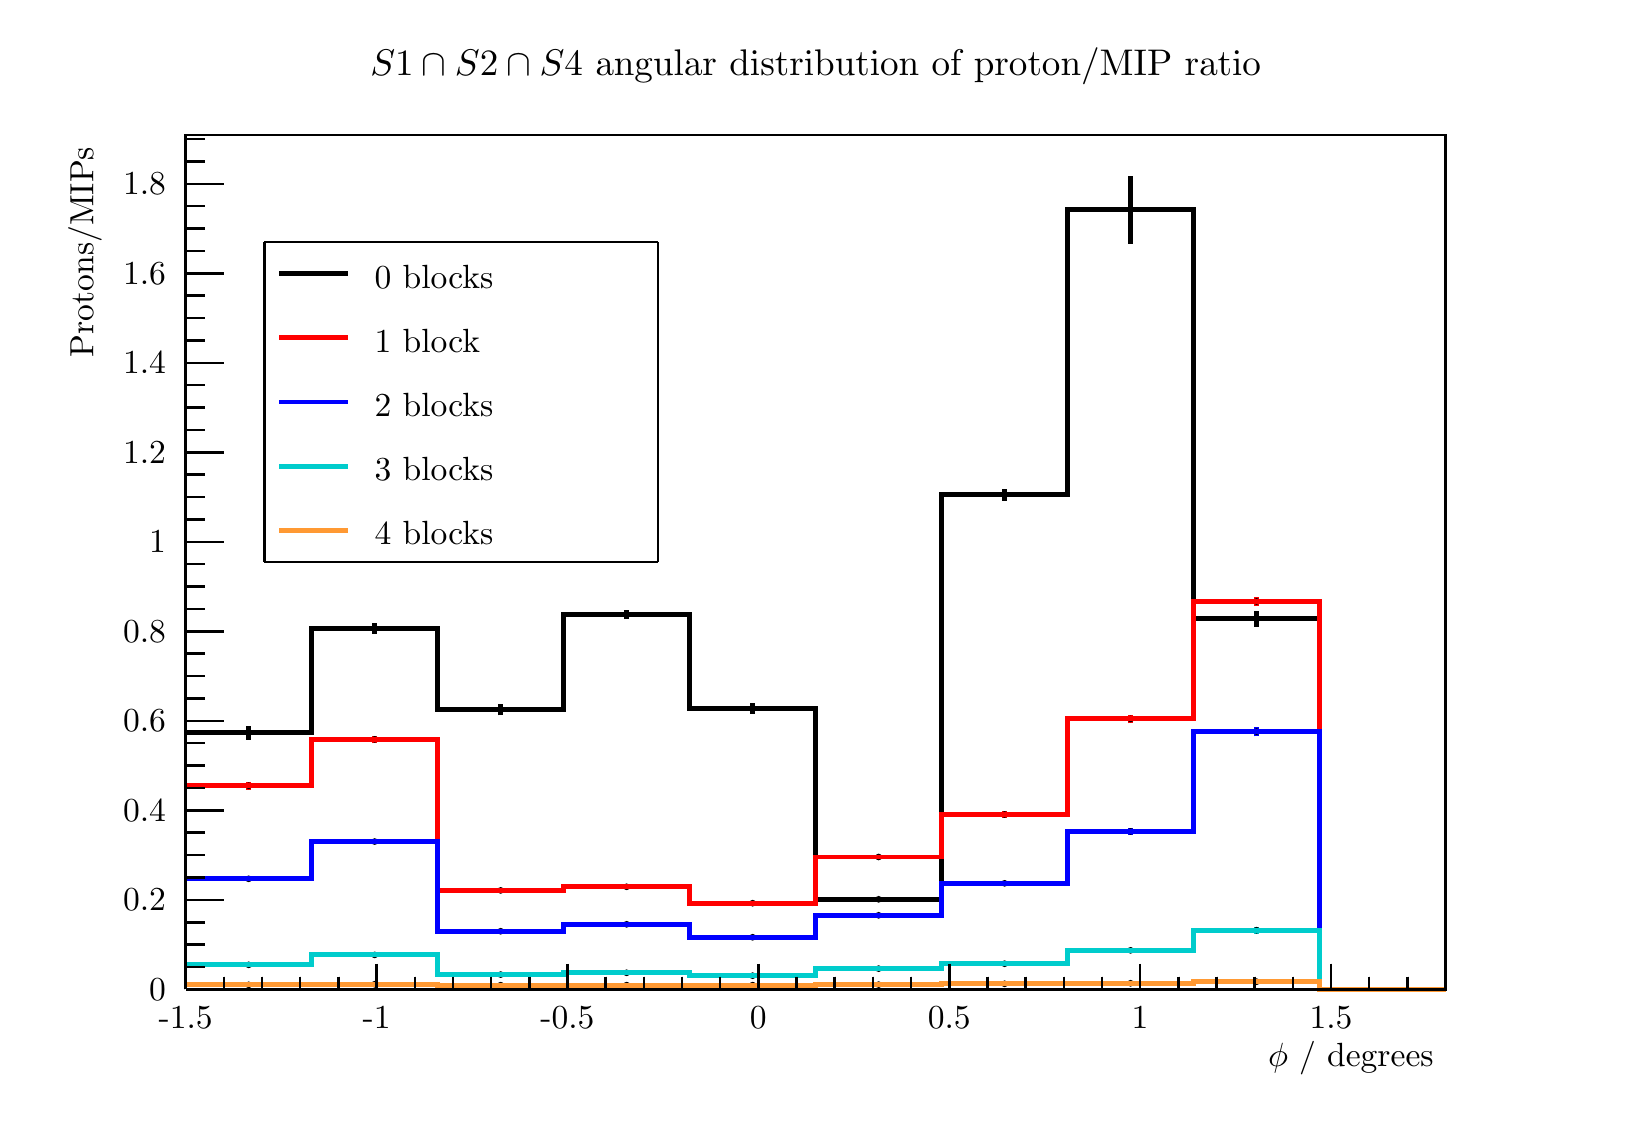
\begin{tikzpicture}
\pgfdeclareplotmark{cross} {
\pgfpathmoveto{\pgfpoint{-0.3\pgfplotmarksize}{\pgfplotmarksize}}
\pgfpathlineto{\pgfpoint{+0.3\pgfplotmarksize}{\pgfplotmarksize}}
\pgfpathlineto{\pgfpoint{+0.3\pgfplotmarksize}{0.3\pgfplotmarksize}}
\pgfpathlineto{\pgfpoint{+1\pgfplotmarksize}{0.3\pgfplotmarksize}}
\pgfpathlineto{\pgfpoint{+1\pgfplotmarksize}{-0.3\pgfplotmarksize}}
\pgfpathlineto{\pgfpoint{+0.3\pgfplotmarksize}{-0.3\pgfplotmarksize}}
\pgfpathlineto{\pgfpoint{+0.3\pgfplotmarksize}{-1.\pgfplotmarksize}}
\pgfpathlineto{\pgfpoint{-0.3\pgfplotmarksize}{-1.\pgfplotmarksize}}
\pgfpathlineto{\pgfpoint{-0.3\pgfplotmarksize}{-0.3\pgfplotmarksize}}
\pgfpathlineto{\pgfpoint{-1.\pgfplotmarksize}{-0.3\pgfplotmarksize}}
\pgfpathlineto{\pgfpoint{-1.\pgfplotmarksize}{0.3\pgfplotmarksize}}
\pgfpathlineto{\pgfpoint{-0.3\pgfplotmarksize}{0.3\pgfplotmarksize}}
\pgfpathclose
\pgfusepathqstroke
}
\pgfdeclareplotmark{cross*} {
\pgfpathmoveto{\pgfpoint{-0.3\pgfplotmarksize}{\pgfplotmarksize}}
\pgfpathlineto{\pgfpoint{+0.3\pgfplotmarksize}{\pgfplotmarksize}}
\pgfpathlineto{\pgfpoint{+0.3\pgfplotmarksize}{0.3\pgfplotmarksize}}
\pgfpathlineto{\pgfpoint{+1\pgfplotmarksize}{0.3\pgfplotmarksize}}
\pgfpathlineto{\pgfpoint{+1\pgfplotmarksize}{-0.3\pgfplotmarksize}}
\pgfpathlineto{\pgfpoint{+0.3\pgfplotmarksize}{-0.3\pgfplotmarksize}}
\pgfpathlineto{\pgfpoint{+0.3\pgfplotmarksize}{-1.\pgfplotmarksize}}
\pgfpathlineto{\pgfpoint{-0.3\pgfplotmarksize}{-1.\pgfplotmarksize}}
\pgfpathlineto{\pgfpoint{-0.3\pgfplotmarksize}{-0.3\pgfplotmarksize}}
\pgfpathlineto{\pgfpoint{-1.\pgfplotmarksize}{-0.3\pgfplotmarksize}}
\pgfpathlineto{\pgfpoint{-1.\pgfplotmarksize}{0.3\pgfplotmarksize}}
\pgfpathlineto{\pgfpoint{-0.3\pgfplotmarksize}{0.3\pgfplotmarksize}}
\pgfpathclose
\pgfusepathqfillstroke
}
\pgfdeclareplotmark{newstar} {
\pgfpathmoveto{\pgfqpoint{0pt}{\pgfplotmarksize}}
\pgfpathlineto{\pgfqpointpolar{44}{0.5\pgfplotmarksize}}
\pgfpathlineto{\pgfqpointpolar{18}{\pgfplotmarksize}}
\pgfpathlineto{\pgfqpointpolar{-20}{0.5\pgfplotmarksize}}
\pgfpathlineto{\pgfqpointpolar{-54}{\pgfplotmarksize}}
\pgfpathlineto{\pgfqpointpolar{-90}{0.5\pgfplotmarksize}}
\pgfpathlineto{\pgfqpointpolar{234}{\pgfplotmarksize}}
\pgfpathlineto{\pgfqpointpolar{198}{0.5\pgfplotmarksize}}
\pgfpathlineto{\pgfqpointpolar{162}{\pgfplotmarksize}}
\pgfpathlineto{\pgfqpointpolar{134}{0.5\pgfplotmarksize}}
\pgfpathclose
\pgfusepathqstroke
}
\pgfdeclareplotmark{newstar*} {
\pgfpathmoveto{\pgfqpoint{0pt}{\pgfplotmarksize}}
\pgfpathlineto{\pgfqpointpolar{44}{0.5\pgfplotmarksize}}
\pgfpathlineto{\pgfqpointpolar{18}{\pgfplotmarksize}}
\pgfpathlineto{\pgfqpointpolar{-20}{0.5\pgfplotmarksize}}
\pgfpathlineto{\pgfqpointpolar{-54}{\pgfplotmarksize}}
\pgfpathlineto{\pgfqpointpolar{-90}{0.5\pgfplotmarksize}}
\pgfpathlineto{\pgfqpointpolar{234}{\pgfplotmarksize}}
\pgfpathlineto{\pgfqpointpolar{198}{0.5\pgfplotmarksize}}
\pgfpathlineto{\pgfqpointpolar{162}{\pgfplotmarksize}}
\pgfpathlineto{\pgfqpointpolar{134}{0.5\pgfplotmarksize}}
\pgfpathclose
\pgfusepathqfillstroke
}
\definecolor{c}{rgb}{1,1,1};
\draw [color=c, fill=c] (0,0) rectangle (20,13.5632);
\draw [color=c, fill=c] (2,1.35632) rectangle (18,12.2069);
\definecolor{c}{rgb}{0,0,0};
\draw [c,line width=0.9] (2,1.35632) -- (2,12.2069) -- (18,12.2069) -- (18,1.35632) -- (2,1.35632);
\definecolor{c}{rgb}{1,1,1};
\draw [color=c, fill=c] (2,1.35632) rectangle (18,12.2069);
\definecolor{c}{rgb}{0,0,0};
\draw [c,line width=0.9] (2,1.35632) -- (2,12.2069) -- (18,12.2069) -- (18,1.35632) -- (2,1.35632);
\definecolor{c}{rgb}{0,0,0.6};
\draw [c,line width=0.9] (2,1.35632) -- (3.6,1.35632) -- (3.6,1.35632) -- (5.2,1.35632) -- (5.2,1.35632) -- (6.8,1.35632) -- (6.8,1.35632) -- (8.4,1.35632) -- (8.4,1.35632) -- (10,1.35632) -- (10,1.35632) -- (11.6,1.35632) -- (11.6,1.35632) --
 (13.2,1.35632) -- (13.2,1.35632) -- (14.8,1.35632) -- (14.8,1.35632) -- (16.4,1.35632) -- (16.4,1.35632) -- (18,1.35632);
\definecolor{c}{rgb}{0,0,0};
\draw [c,line width=0.9] (2,1.35632) -- (18,1.35632);
\draw [anchor= east] (18,0.488276) node[scale=1.2126, color=c, rotate=0]{$ \phi$ / degrees};
\draw [c,line width=0.9] (2,1.68184) -- (2,1.35632);
\draw [c,line width=0.9] (2.48485,1.51908) -- (2.48485,1.35632);
\draw [c,line width=0.9] (2.9697,1.51908) -- (2.9697,1.35632);
\draw [c,line width=0.9] (3.45455,1.51908) -- (3.45455,1.35632);
\draw [c,line width=0.9] (3.93939,1.51908) -- (3.93939,1.35632);
\draw [c,line width=0.9] (4.42424,1.68184) -- (4.42424,1.35632);
\draw [c,line width=0.9] (4.90909,1.51908) -- (4.90909,1.35632);
\draw [c,line width=0.9] (5.39394,1.51908) -- (5.39394,1.35632);
\draw [c,line width=0.9] (5.87879,1.51908) -- (5.87879,1.35632);
\draw [c,line width=0.9] (6.36364,1.51908) -- (6.36364,1.35632);
\draw [c,line width=0.9] (6.84848,1.68184) -- (6.84848,1.35632);
\draw [c,line width=0.9] (7.33333,1.51908) -- (7.33333,1.35632);
\draw [c,line width=0.9] (7.81818,1.51908) -- (7.81818,1.35632);
\draw [c,line width=0.9] (8.30303,1.51908) -- (8.30303,1.35632);
\draw [c,line width=0.9] (8.78788,1.51908) -- (8.78788,1.35632);
\draw [c,line width=0.9] (9.27273,1.68184) -- (9.27273,1.35632);
\draw [c,line width=0.9] (9.75758,1.51908) -- (9.75758,1.35632);
\draw [c,line width=0.9] (10.2424,1.51908) -- (10.2424,1.35632);
\draw [c,line width=0.9] (10.7273,1.51908) -- (10.7273,1.35632);
\draw [c,line width=0.9] (11.2121,1.51908) -- (11.2121,1.35632);
\draw [c,line width=0.9] (11.697,1.68184) -- (11.697,1.35632);
\draw [c,line width=0.9] (12.1818,1.51908) -- (12.1818,1.35632);
\draw [c,line width=0.9] (12.6667,1.51908) -- (12.6667,1.35632);
\draw [c,line width=0.9] (13.1515,1.51908) -- (13.1515,1.35632);
\draw [c,line width=0.9] (13.6364,1.51908) -- (13.6364,1.35632);
\draw [c,line width=0.9] (14.1212,1.68184) -- (14.1212,1.35632);
\draw [c,line width=0.9] (14.6061,1.51908) -- (14.6061,1.35632);
\draw [c,line width=0.9] (15.0909,1.51908) -- (15.0909,1.35632);
\draw [c,line width=0.9] (15.5758,1.51908) -- (15.5758,1.35632);
\draw [c,line width=0.9] (16.0606,1.51908) -- (16.0606,1.35632);
\draw [c,line width=0.9] (16.5455,1.68184) -- (16.5455,1.35632);
\draw [c,line width=0.9] (16.5455,1.68184) -- (16.5455,1.35632);
\draw [c,line width=0.9] (17.0303,1.51908) -- (17.0303,1.35632);
\draw [c,line width=0.9] (17.5152,1.51908) -- (17.5152,1.35632);
\draw [c,line width=0.9] (18,1.51908) -- (18,1.35632);
\draw [anchor=base] (2,0.854483) node[scale=1.2126, color=c, rotate=0]{-1.5};
\draw [anchor=base] (4.42424,0.854483) node[scale=1.2126, color=c, rotate=0]{-1};
\draw [anchor=base] (6.84848,0.854483) node[scale=1.2126, color=c, rotate=0]{-0.5};
\draw [anchor=base] (9.27273,0.854483) node[scale=1.2126, color=c, rotate=0]{0};
\draw [anchor=base] (11.697,0.854483) node[scale=1.2126, color=c, rotate=0]{0.5};
\draw [anchor=base] (14.1212,0.854483) node[scale=1.2126, color=c, rotate=0]{1};
\draw [anchor=base] (16.5455,0.854483) node[scale=1.2126, color=c, rotate=0]{1.5};
\draw [c,line width=0.9] (2,1.35632) -- (2,12.2069);
\draw [anchor= east] (0.72,12.2069) node[scale=1.2126, color=c, rotate=90]{ Protons/MIPs};
\draw [c,line width=0.9] (2.48,1.35632) -- (2,1.35632);
\draw [c,line width=0.9] (2.24,1.64053) -- (2,1.64053);
\draw [c,line width=0.9] (2.24,1.92473) -- (2,1.92473);
\draw [c,line width=0.9] (2.24,2.20894) -- (2,2.20894);
\draw [c,line width=0.9] (2.48,2.49314) -- (2,2.49314);
\draw [c,line width=0.9] (2.24,2.77735) -- (2,2.77735);
\draw [c,line width=0.9] (2.24,3.06155) -- (2,3.06155);
\draw [c,line width=0.9] (2.24,3.34576) -- (2,3.34576);
\draw [c,line width=0.9] (2.48,3.62996) -- (2,3.62996);
\draw [c,line width=0.9] (2.24,3.91417) -- (2,3.91417);
\draw [c,line width=0.9] (2.24,4.19837) -- (2,4.19837);
\draw [c,line width=0.9] (2.24,4.48258) -- (2,4.48258);
\draw [c,line width=0.9] (2.48,4.76678) -- (2,4.76678);
\draw [c,line width=0.9] (2.24,5.05099) -- (2,5.05099);
\draw [c,line width=0.9] (2.24,5.33519) -- (2,5.33519);
\draw [c,line width=0.9] (2.24,5.6194) -- (2,5.6194);
\draw [c,line width=0.9] (2.48,5.9036) -- (2,5.9036);
\draw [c,line width=0.9] (2.24,6.18781) -- (2,6.18781);
\draw [c,line width=0.9] (2.24,6.47201) -- (2,6.47201);
\draw [c,line width=0.9] (2.24,6.75622) -- (2,6.75622);
\draw [c,line width=0.9] (2.48,7.04042) -- (2,7.04042);
\draw [c,line width=0.9] (2.24,7.32463) -- (2,7.32463);
\draw [c,line width=0.9] (2.24,7.60883) -- (2,7.60883);
\draw [c,line width=0.9] (2.24,7.89304) -- (2,7.89304);
\draw [c,line width=0.9] (2.48,8.17724) -- (2,8.17724);
\draw [c,line width=0.9] (2.24,8.46145) -- (2,8.46145);
\draw [c,line width=0.9] (2.24,8.74565) -- (2,8.74565);
\draw [c,line width=0.9] (2.24,9.02986) -- (2,9.02986);
\draw [c,line width=0.9] (2.48,9.31406) -- (2,9.31406);
\draw [c,line width=0.9] (2.24,9.59827) -- (2,9.59827);
\draw [c,line width=0.9] (2.24,9.88247) -- (2,9.88247);
\draw [c,line width=0.9] (2.24,10.1667) -- (2,10.1667);
\draw [c,line width=0.9] (2.48,10.4509) -- (2,10.4509);
\draw [c,line width=0.9] (2.24,10.7351) -- (2,10.7351);
\draw [c,line width=0.9] (2.24,11.0193) -- (2,11.0193);
\draw [c,line width=0.9] (2.24,11.3035) -- (2,11.3035);
\draw [c,line width=0.9] (2.48,11.5877) -- (2,11.5877);
\draw [c,line width=0.9] (2.48,11.5877) -- (2,11.5877);
\draw [c,line width=0.9] (2.24,11.8719) -- (2,11.8719);
\draw [c,line width=0.9] (2.24,12.1561) -- (2,12.1561);
\draw [anchor= east] (1.9,1.35632) node[scale=1.2126, color=c, rotate=0]{0};
\draw [anchor= east] (1.9,2.49314) node[scale=1.2126, color=c, rotate=0]{0.2};
\draw [anchor= east] (1.9,3.62996) node[scale=1.2126, color=c, rotate=0]{0.4};
\draw [anchor= east] (1.9,4.76678) node[scale=1.2126, color=c, rotate=0]{0.6};
\draw [anchor= east] (1.9,5.9036) node[scale=1.2126, color=c, rotate=0]{0.8};
\draw [anchor= east] (1.9,7.04042) node[scale=1.2126, color=c, rotate=0]{1};
\draw [anchor= east] (1.9,8.17724) node[scale=1.2126, color=c, rotate=0]{1.2};
\draw [anchor= east] (1.9,9.31406) node[scale=1.2126, color=c, rotate=0]{1.4};
\draw [anchor= east] (1.9,10.4509) node[scale=1.2126, color=c, rotate=0]{1.6};
\draw [anchor= east] (1.9,11.5877) node[scale=1.2126, color=c, rotate=0]{1.8};
\draw [c,line width=1.8] (2.8,4.52786) -- (2.8,4.61649);
\draw [c,line width=1.8] (2.8,4.61649) -- (2.8,4.70512);
\foreach \P in {(2.8,4.61649)}{\draw[mark options={color=c,fill=c},mark size=2.402402pt,mark=*,mark size=1pt] plot coordinates {\P};}
\draw [c,line width=1.8] (4.4,5.87328) -- (4.4,5.94218);
\draw [c,line width=1.8] (4.4,5.94218) -- (4.4,6.01107);
\foreach \P in {(4.4,5.94218)}{\draw[mark options={color=c,fill=c},mark size=2.402402pt,mark=*,mark size=1pt] plot coordinates {\P};}
\draw [c,line width=1.8] (6,4.83657) -- (6,4.90889);
\draw [c,line width=1.8] (6,4.90889) -- (6,4.9812);
\foreach \P in {(6,4.90889)}{\draw[mark options={color=c,fill=c},mark size=2.402402pt,mark=*,mark size=1pt] plot coordinates {\P};}
\draw [c,line width=1.8] (7.6,6.05742) -- (7.6,6.11289);
\draw [c,line width=1.8] (7.6,6.11289) -- (7.6,6.16836);
\foreach \P in {(7.6,6.11289)}{\draw[mark options={color=c,fill=c},mark size=2.402402pt,mark=*,mark size=1pt] plot coordinates {\P};}
\draw [c,line width=1.8] (9.2,4.85848) -- (9.2,4.92525);
\draw [c,line width=1.8] (9.2,4.92525) -- (9.2,4.99203);
\foreach \P in {(9.2,4.92525)}{\draw[mark options={color=c,fill=c},mark size=2.402402pt,mark=*,mark size=1pt] plot coordinates {\P};}
\draw [c,line width=1.8] (10.8,2.46997) -- (10.8,2.50047);
\draw [c,line width=1.8] (10.8,2.50047) -- (10.8,2.53097);
\foreach \P in {(10.8,2.50047)}{\draw[mark options={color=c,fill=c},mark size=2.402402pt,mark=*,mark size=1pt] plot coordinates {\P};}
\draw [c,line width=1.8] (12.4,7.56489) -- (12.4,7.6379);
\draw [c,line width=1.8] (12.4,7.6379) -- (12.4,7.71091);
\foreach \P in {(12.4,7.6379)}{\draw[mark options={color=c,fill=c},mark size=2.402402pt,mark=*,mark size=1pt] plot coordinates {\P};}
\draw [c,line width=1.8] (14,10.8284) -- (14,11.2593);
\draw [c,line width=1.8] (14,11.2593) -- (14,11.6902);
\foreach \P in {(14,11.2593)}{\draw[mark options={color=c,fill=c},mark size=2.402402pt,mark=*,mark size=1pt] plot coordinates {\P};}
\draw [c,line width=1.8] (15.6,5.9618) -- (15.6,6.06082);
\draw [c,line width=1.8] (15.6,6.06082) -- (15.6,6.15984);
\foreach \P in {(15.6,6.06082)}{\draw[mark options={color=c,fill=c},mark size=2.402402pt,mark=*,mark size=1pt] plot coordinates {\P};}
\draw [c,line width=1.8] (2,4.61649) -- (3.6,4.61649) -- (3.6,5.94218) -- (5.2,5.94218) -- (5.2,4.90889) -- (6.8,4.90889) -- (6.8,6.11289) -- (8.4,6.11289) -- (8.4,4.92525) -- (10,4.92525) -- (10,2.50047) -- (11.6,2.50047) -- (11.6,7.6379) --
 (13.2,7.6379) -- (13.2,11.2593) -- (14.8,11.2593) -- (14.8,6.06082) -- (16.4,6.06082) -- (16.4,1.35632) -- (18,1.35632);
\definecolor{c}{rgb}{1,0,0};
\draw [c,line width=1.8] (2.8,3.89168) -- (2.8,3.94269);
\draw [c,line width=1.8] (2.8,3.94269) -- (2.8,3.9937);
\definecolor{c}{rgb}{0,0,0};
\foreach \P in {(2.8,3.94269)}{\draw[mark options={color=c,fill=c},mark size=2.402402pt,mark=*,mark size=1pt] plot coordinates {\P};}
\definecolor{c}{rgb}{1,0,0};
\draw [c,line width=1.8] (4.4,4.4836) -- (4.4,4.53195);
\draw [c,line width=1.8] (4.4,4.53195) -- (4.4,4.58029);
\definecolor{c}{rgb}{0,0,0};
\foreach \P in {(4.4,4.53195)}{\draw[mark options={color=c,fill=c},mark size=2.402402pt,mark=*,mark size=1pt] plot coordinates {\P};}
\definecolor{c}{rgb}{1,0,0};
\draw [c,line width=1.8] (6,2.58936) -- (6,2.61337);
\draw [c,line width=1.8] (6,2.61337) -- (6,2.63738);
\definecolor{c}{rgb}{0,0,0};
\foreach \P in {(6,2.61337)}{\draw[mark options={color=c,fill=c},mark size=2.402402pt,mark=*,mark size=1pt] plot coordinates {\P};}
\definecolor{c}{rgb}{1,0,0};
\draw [c,line width=1.8] (7.6,2.63677) -- (7.6,2.65956);
\draw [c,line width=1.8] (7.6,2.65956) -- (7.6,2.68236);
\definecolor{c}{rgb}{0,0,0};
\foreach \P in {(7.6,2.65956)}{\draw[mark options={color=c,fill=c},mark size=2.402402pt,mark=*,mark size=1pt] plot coordinates {\P};}
\definecolor{c}{rgb}{1,0,0};
\draw [c,line width=1.8] (9.2,2.43084) -- (9.2,2.45105);
\draw [c,line width=1.8] (9.2,2.45105) -- (9.2,2.47127);
\definecolor{c}{rgb}{0,0,0};
\foreach \P in {(9.2,2.45105)}{\draw[mark options={color=c,fill=c},mark size=2.402402pt,mark=*,mark size=1pt] plot coordinates {\P};}
\definecolor{c}{rgb}{1,0,0};
\draw [c,line width=1.8] (10.8,3.00958) -- (10.8,3.03783);
\draw [c,line width=1.8] (10.8,3.03783) -- (10.8,3.06608);
\definecolor{c}{rgb}{0,0,0};
\foreach \P in {(10.8,3.03783)}{\draw[mark options={color=c,fill=c},mark size=2.402402pt,mark=*,mark size=1pt] plot coordinates {\P};}
\definecolor{c}{rgb}{1,0,0};
\draw [c,line width=1.8] (12.4,3.53763) -- (12.4,3.57752);
\draw [c,line width=1.8] (12.4,3.57752) -- (12.4,3.61741);
\definecolor{c}{rgb}{0,0,0};
\foreach \P in {(12.4,3.57752)}{\draw[mark options={color=c,fill=c},mark size=2.402402pt,mark=*,mark size=1pt] plot coordinates {\P};}
\definecolor{c}{rgb}{1,0,0};
\draw [c,line width=1.8] (14,4.73628) -- (14,4.79116);
\draw [c,line width=1.8] (14,4.79116) -- (14,4.84604);
\definecolor{c}{rgb}{0,0,0};
\foreach \P in {(14,4.79116)}{\draw[mark options={color=c,fill=c},mark size=2.402402pt,mark=*,mark size=1pt] plot coordinates {\P};}
\definecolor{c}{rgb}{1,0,0};
\draw [c,line width=1.8] (15.6,6.2245) -- (15.6,6.28324);
\draw [c,line width=1.8] (15.6,6.28324) -- (15.6,6.34199);
\definecolor{c}{rgb}{0,0,0};
\foreach \P in {(15.6,6.28324)}{\draw[mark options={color=c,fill=c},mark size=2.402402pt,mark=*,mark size=1pt] plot coordinates {\P};}
\definecolor{c}{rgb}{1,0,0};
\draw [c,line width=1.8] (2,3.94269) -- (3.6,3.94269) -- (3.6,4.53195) -- (5.2,4.53195) -- (5.2,2.61337) -- (6.8,2.61337) -- (6.8,2.65956) -- (8.4,2.65956) -- (8.4,2.45105) -- (10,2.45105) -- (10,3.03783) -- (11.6,3.03783) -- (11.6,3.57752) --
 (13.2,3.57752) -- (13.2,4.79116) -- (14.8,4.79116) -- (14.8,6.28324) -- (16.4,6.28324) -- (16.4,1.35632) -- (18,1.35632);
\definecolor{c}{rgb}{0,0,1};
\draw [c,line width=1.8] (2.8,2.7273) -- (2.8,2.76072);
\draw [c,line width=1.8] (2.8,2.76072) -- (2.8,2.79413);
\definecolor{c}{rgb}{0,0,0};
\foreach \P in {(2.8,2.76072)}{\draw[mark options={color=c,fill=c},mark size=2.402402pt,mark=*,mark size=1pt] plot coordinates {\P};}
\definecolor{c}{rgb}{0,0,1};
\draw [c,line width=1.8] (4.4,3.1989) -- (4.4,3.23402);
\draw [c,line width=1.8] (4.4,3.23402) -- (4.4,3.26914);
\definecolor{c}{rgb}{0,0,0};
\foreach \P in {(4.4,3.23402)}{\draw[mark options={color=c,fill=c},mark size=2.402402pt,mark=*,mark size=1pt] plot coordinates {\P};}
\definecolor{c}{rgb}{0,0,1};
\draw [c,line width=1.8] (6,2.07976) -- (6,2.09479);
\draw [c,line width=1.8] (6,2.09479) -- (6,2.10982);
\definecolor{c}{rgb}{0,0,0};
\foreach \P in {(6,2.09479)}{\draw[mark options={color=c,fill=c},mark size=2.402402pt,mark=*,mark size=1pt] plot coordinates {\P};}
\definecolor{c}{rgb}{0,0,1};
\draw [c,line width=1.8] (7.6,2.16804) -- (7.6,2.18299);
\draw [c,line width=1.8] (7.6,2.18299) -- (7.6,2.19795);
\definecolor{c}{rgb}{0,0,0};
\foreach \P in {(7.6,2.18299)}{\draw[mark options={color=c,fill=c},mark size=2.402402pt,mark=*,mark size=1pt] plot coordinates {\P};}
\definecolor{c}{rgb}{0,0,1};
\draw [c,line width=1.8] (9.2,2.00565) -- (9.2,2.01848);
\draw [c,line width=1.8] (9.2,2.01848) -- (9.2,2.03132);
\definecolor{c}{rgb}{0,0,0};
\foreach \P in {(9.2,2.01848)}{\draw[mark options={color=c,fill=c},mark size=2.402402pt,mark=*,mark size=1pt] plot coordinates {\P};}
\definecolor{c}{rgb}{0,0,1};
\draw [c,line width=1.8] (10.8,2.27928) -- (10.8,2.29724);
\draw [c,line width=1.8] (10.8,2.29724) -- (10.8,2.3152);
\definecolor{c}{rgb}{0,0,0};
\foreach \P in {(10.8,2.29724)}{\draw[mark options={color=c,fill=c},mark size=2.402402pt,mark=*,mark size=1pt] plot coordinates {\P};}
\definecolor{c}{rgb}{0,0,1};
\draw [c,line width=1.8] (12.4,2.67601) -- (12.4,2.70318);
\draw [c,line width=1.8] (12.4,2.70318) -- (12.4,2.73035);
\definecolor{c}{rgb}{0,0,0};
\foreach \P in {(12.4,2.70318)}{\draw[mark options={color=c,fill=c},mark size=2.402402pt,mark=*,mark size=1pt] plot coordinates {\P};}
\definecolor{c}{rgb}{0,0,1};
\draw [c,line width=1.8] (14,3.32317) -- (14,3.3629);
\draw [c,line width=1.8] (14,3.3629) -- (14,3.40264);
\definecolor{c}{rgb}{0,0,0};
\foreach \P in {(14,3.3629)}{\draw[mark options={color=c,fill=c},mark size=2.402402pt,mark=*,mark size=1pt] plot coordinates {\P};}
\definecolor{c}{rgb}{0,0,1};
\draw [c,line width=1.8] (15.6,4.56937) -- (15.6,4.63071);
\draw [c,line width=1.8] (15.6,4.63071) -- (15.6,4.69205);
\definecolor{c}{rgb}{0,0,0};
\foreach \P in {(15.6,4.63071)}{\draw[mark options={color=c,fill=c},mark size=2.402402pt,mark=*,mark size=1pt] plot coordinates {\P};}
\definecolor{c}{rgb}{0,0,1};
\draw [c,line width=1.8] (2,2.76072) -- (3.6,2.76072) -- (3.6,3.23402) -- (5.2,3.23402) -- (5.2,2.09479) -- (6.8,2.09479) -- (6.8,2.18299) -- (8.4,2.18299) -- (8.4,2.01848) -- (10,2.01848) -- (10,2.29724) -- (11.6,2.29724) -- (11.6,2.70318) --
 (13.2,2.70318) -- (13.2,3.3629) -- (14.8,3.3629) -- (14.8,4.63071) -- (16.4,4.63071) -- (16.4,1.35632) -- (18,1.35632);
\definecolor{c}{rgb}{0,0.8,0.8};
\draw [c,line width=1.8] (2.8,1.65005) -- (2.8,1.66824);
\draw [c,line width=1.8] (2.8,1.66824) -- (2.8,1.68643);
\definecolor{c}{rgb}{0,0,0};
\foreach \P in {(2.8,1.66824)}{\draw[mark options={color=c,fill=c},mark size=2.402402pt,mark=*,mark size=1pt] plot coordinates {\P};}
\definecolor{c}{rgb}{0,0.8,0.8};
\draw [c,line width=1.8] (4.4,1.77412) -- (4.4,1.7946);
\draw [c,line width=1.8] (4.4,1.7946) -- (4.4,1.81507);
\definecolor{c}{rgb}{0,0,0};
\foreach \P in {(4.4,1.7946)}{\draw[mark options={color=c,fill=c},mark size=2.402402pt,mark=*,mark size=1pt] plot coordinates {\P};}
\definecolor{c}{rgb}{0,0.8,0.8};
\draw [c,line width=1.8] (6,1.53592) -- (6,1.54425);
\draw [c,line width=1.8] (6,1.54425) -- (6,1.55258);
\definecolor{c}{rgb}{0,0,0};
\foreach \P in {(6,1.54425)}{\draw[mark options={color=c,fill=c},mark size=2.402402pt,mark=*,mark size=1pt] plot coordinates {\P};}
\definecolor{c}{rgb}{0,0.8,0.8};
\draw [c,line width=1.8] (7.6,1.55892) -- (7.6,1.56732);
\draw [c,line width=1.8] (7.6,1.56732) -- (7.6,1.57572);
\definecolor{c}{rgb}{0,0,0};
\foreach \P in {(7.6,1.56732)}{\draw[mark options={color=c,fill=c},mark size=2.402402pt,mark=*,mark size=1pt] plot coordinates {\P};}
\definecolor{c}{rgb}{0,0.8,0.8};
\draw [c,line width=1.8] (9.2,1.52312) -- (9.2,1.53036);
\draw [c,line width=1.8] (9.2,1.53036) -- (9.2,1.5376);
\definecolor{c}{rgb}{0,0,0};
\foreach \P in {(9.2,1.53036)}{\draw[mark options={color=c,fill=c},mark size=2.402402pt,mark=*,mark size=1pt] plot coordinates {\P};}
\definecolor{c}{rgb}{0,0.8,0.8};
\draw [c,line width=1.8] (10.8,1.60929) -- (10.8,1.61987);
\draw [c,line width=1.8] (10.8,1.61987) -- (10.8,1.63045);
\definecolor{c}{rgb}{0,0,0};
\foreach \P in {(10.8,1.61987)}{\draw[mark options={color=c,fill=c},mark size=2.402402pt,mark=*,mark size=1pt] plot coordinates {\P};}
\definecolor{c}{rgb}{0,0.8,0.8};
\draw [c,line width=1.8] (12.4,1.66665) -- (12.4,1.68218);
\draw [c,line width=1.8] (12.4,1.68218) -- (12.4,1.69771);
\definecolor{c}{rgb}{0,0,0};
\foreach \P in {(12.4,1.68218)}{\draw[mark options={color=c,fill=c},mark size=2.402402pt,mark=*,mark size=1pt] plot coordinates {\P};}
\definecolor{c}{rgb}{0,0.8,0.8};
\draw [c,line width=1.8] (14,1.82799) -- (14,1.85229);
\draw [c,line width=1.8] (14,1.85229) -- (14,1.8766);
\definecolor{c}{rgb}{0,0,0};
\foreach \P in {(14,1.85229)}{\draw[mark options={color=c,fill=c},mark size=2.402402pt,mark=*,mark size=1pt] plot coordinates {\P};}
\definecolor{c}{rgb}{0,0.8,0.8};
\draw [c,line width=1.8] (15.6,2.06381) -- (15.6,2.10801);
\draw [c,line width=1.8] (15.6,2.10801) -- (15.6,2.15221);
\definecolor{c}{rgb}{0,0,0};
\foreach \P in {(15.6,2.10801)}{\draw[mark options={color=c,fill=c},mark size=2.402402pt,mark=*,mark size=1pt] plot coordinates {\P};}
\definecolor{c}{rgb}{0,0.8,0.8};
\draw [c,line width=1.8] (2,1.66824) -- (3.6,1.66824) -- (3.6,1.7946) -- (5.2,1.7946) -- (5.2,1.54425) -- (6.8,1.54425) -- (6.8,1.56732) -- (8.4,1.56732) -- (8.4,1.53036) -- (10,1.53036) -- (10,1.61987) -- (11.6,1.61987) -- (11.6,1.68218) --
 (13.2,1.68218) -- (13.2,1.85229) -- (14.8,1.85229) -- (14.8,2.10801) -- (16.4,2.10801) -- (16.4,1.35632) -- (18,1.35632);
\definecolor{c}{rgb}{1,0.6,0.2};
\draw [c,line width=1.8] (2.8,1.41274) -- (2.8,1.41433);
\draw [c,line width=1.8] (2.8,1.41433) -- (2.8,1.41592);
\definecolor{c}{rgb}{0,0,0};
\foreach \P in {(2.8,1.41433)}{\draw[mark options={color=c,fill=c},mark size=2.402402pt,mark=*,mark size=1pt] plot coordinates {\P};}
\definecolor{c}{rgb}{1,0.6,0.2};
\draw [c,line width=1.8] (4.4,1.42029) -- (4.4,1.42182);
\draw [c,line width=1.8] (4.4,1.42182) -- (4.4,1.42336);
\definecolor{c}{rgb}{0,0,0};
\foreach \P in {(4.4,1.42182)}{\draw[mark options={color=c,fill=c},mark size=2.402402pt,mark=*,mark size=1pt] plot coordinates {\P};}
\definecolor{c}{rgb}{1,0.6,0.2};
\draw [c,line width=1.8] (6,1.40859) -- (6,1.40946);
\draw [c,line width=1.8] (6,1.40946) -- (6,1.41033);
\definecolor{c}{rgb}{0,0,0};
\foreach \P in {(6,1.40946)}{\draw[mark options={color=c,fill=c},mark size=2.402402pt,mark=*,mark size=1pt] plot coordinates {\P};}
\definecolor{c}{rgb}{1,0.6,0.2};
\draw [c,line width=1.8] (7.6,1.40953) -- (7.6,1.41037);
\draw [c,line width=1.8] (7.6,1.41037) -- (7.6,1.41122);
\definecolor{c}{rgb}{0,0,0};
\foreach \P in {(7.6,1.41037)}{\draw[mark options={color=c,fill=c},mark size=2.402402pt,mark=*,mark size=1pt] plot coordinates {\P};}
\definecolor{c}{rgb}{1,0.6,0.2};
\draw [c,line width=1.8] (9.2,1.40941) -- (9.2,1.41022);
\draw [c,line width=1.8] (9.2,1.41022) -- (9.2,1.41102);
\definecolor{c}{rgb}{0,0,0};
\foreach \P in {(9.2,1.41022)}{\draw[mark options={color=c,fill=c},mark size=2.402402pt,mark=*,mark size=1pt] plot coordinates {\P};}
\definecolor{c}{rgb}{1,0.6,0.2};
\draw [c,line width=1.8] (10.8,1.41566) -- (10.8,1.41668);
\draw [c,line width=1.8] (10.8,1.41668) -- (10.8,1.4177);
\definecolor{c}{rgb}{0,0,0};
\foreach \P in {(10.8,1.41668)}{\draw[mark options={color=c,fill=c},mark size=2.402402pt,mark=*,mark size=1pt] plot coordinates {\P};}
\definecolor{c}{rgb}{1,0.6,0.2};
\draw [c,line width=1.8] (12.4,1.4259) -- (12.4,1.42736);
\draw [c,line width=1.8] (12.4,1.42736) -- (12.4,1.42883);
\definecolor{c}{rgb}{0,0,0};
\foreach \P in {(12.4,1.42736)}{\draw[mark options={color=c,fill=c},mark size=2.402402pt,mark=*,mark size=1pt] plot coordinates {\P};}
\definecolor{c}{rgb}{1,0.6,0.2};
\draw [c,line width=1.8] (14,1.43199) -- (14,1.43389);
\draw [c,line width=1.8] (14,1.43389) -- (14,1.43578);
\definecolor{c}{rgb}{0,0,0};
\foreach \P in {(14,1.43389)}{\draw[mark options={color=c,fill=c},mark size=2.402402pt,mark=*,mark size=1pt] plot coordinates {\P};}
\definecolor{c}{rgb}{1,0.6,0.2};
\draw [c,line width=1.8] (15.6,1.45109) -- (15.6,1.45416);
\draw [c,line width=1.8] (15.6,1.45416) -- (15.6,1.45724);
\definecolor{c}{rgb}{0,0,0};
\foreach \P in {(15.6,1.45416)}{\draw[mark options={color=c,fill=c},mark size=2.402402pt,mark=*,mark size=1pt] plot coordinates {\P};}
\definecolor{c}{rgb}{1,0.6,0.2};
\draw [c,line width=1.8] (2,1.41433) -- (3.6,1.41433) -- (3.6,1.42182) -- (5.2,1.42182) -- (5.2,1.40946) -- (6.8,1.40946) -- (6.8,1.41037) -- (8.4,1.41037) -- (8.4,1.41022) -- (10,1.41022) -- (10,1.41668) -- (11.6,1.41668) -- (11.6,1.42736) --
 (13.2,1.42736) -- (13.2,1.43389) -- (14.8,1.43389) -- (14.8,1.45416) -- (16.4,1.45416) -- (16.4,1.35632) -- (18,1.35632);
\definecolor{c}{rgb}{0,0,0};
\draw [c,line width=0.9] (2,1.35632) -- (18,1.35632);
\draw [c,line width=0.9] (2,1.68184) -- (2,1.35632);
\draw [c,line width=0.9] (2.48485,1.51908) -- (2.48485,1.35632);
\draw [c,line width=0.9] (2.9697,1.51908) -- (2.9697,1.35632);
\draw [c,line width=0.9] (3.45455,1.51908) -- (3.45455,1.35632);
\draw [c,line width=0.9] (3.93939,1.51908) -- (3.93939,1.35632);
\draw [c,line width=0.9] (4.42424,1.68184) -- (4.42424,1.35632);
\draw [c,line width=0.9] (4.90909,1.51908) -- (4.90909,1.35632);
\draw [c,line width=0.9] (5.39394,1.51908) -- (5.39394,1.35632);
\draw [c,line width=0.9] (5.87879,1.51908) -- (5.87879,1.35632);
\draw [c,line width=0.9] (6.36364,1.51908) -- (6.36364,1.35632);
\draw [c,line width=0.9] (6.84848,1.68184) -- (6.84848,1.35632);
\draw [c,line width=0.9] (7.33333,1.51908) -- (7.33333,1.35632);
\draw [c,line width=0.9] (7.81818,1.51908) -- (7.81818,1.35632);
\draw [c,line width=0.9] (8.30303,1.51908) -- (8.30303,1.35632);
\draw [c,line width=0.9] (8.78788,1.51908) -- (8.78788,1.35632);
\draw [c,line width=0.9] (9.27273,1.68184) -- (9.27273,1.35632);
\draw [c,line width=0.9] (9.75758,1.51908) -- (9.75758,1.35632);
\draw [c,line width=0.9] (10.2424,1.51908) -- (10.2424,1.35632);
\draw [c,line width=0.9] (10.7273,1.51908) -- (10.7273,1.35632);
\draw [c,line width=0.9] (11.2121,1.51908) -- (11.2121,1.35632);
\draw [c,line width=0.9] (11.697,1.68184) -- (11.697,1.35632);
\draw [c,line width=0.9] (12.1818,1.51908) -- (12.1818,1.35632);
\draw [c,line width=0.9] (12.6667,1.51908) -- (12.6667,1.35632);
\draw [c,line width=0.9] (13.1515,1.51908) -- (13.1515,1.35632);
\draw [c,line width=0.9] (13.6364,1.51908) -- (13.6364,1.35632);
\draw [c,line width=0.9] (14.1212,1.68184) -- (14.1212,1.35632);
\draw [c,line width=0.9] (14.6061,1.51908) -- (14.6061,1.35632);
\draw [c,line width=0.9] (15.0909,1.51908) -- (15.0909,1.35632);
\draw [c,line width=0.9] (15.5758,1.51908) -- (15.5758,1.35632);
\draw [c,line width=0.9] (16.0606,1.51908) -- (16.0606,1.35632);
\draw [c,line width=0.9] (16.5455,1.68184) -- (16.5455,1.35632);
\draw [c,line width=0.9] (16.5455,1.68184) -- (16.5455,1.35632);
\draw [c,line width=0.9] (17.0303,1.51908) -- (17.0303,1.35632);
\draw [c,line width=0.9] (17.5152,1.51908) -- (17.5152,1.35632);
\draw [c,line width=0.9] (18,1.51908) -- (18,1.35632);
\draw [c,line width=0.9] (2,1.35632) -- (2,12.2069);
\draw [c,line width=0.9] (2.48,1.35632) -- (2,1.35632);
\draw [c,line width=0.9] (2.24,1.64053) -- (2,1.64053);
\draw [c,line width=0.9] (2.24,1.92473) -- (2,1.92473);
\draw [c,line width=0.9] (2.24,2.20894) -- (2,2.20894);
\draw [c,line width=0.9] (2.48,2.49314) -- (2,2.49314);
\draw [c,line width=0.9] (2.24,2.77735) -- (2,2.77735);
\draw [c,line width=0.9] (2.24,3.06155) -- (2,3.06155);
\draw [c,line width=0.9] (2.24,3.34576) -- (2,3.34576);
\draw [c,line width=0.9] (2.48,3.62996) -- (2,3.62996);
\draw [c,line width=0.9] (2.24,3.91417) -- (2,3.91417);
\draw [c,line width=0.9] (2.24,4.19837) -- (2,4.19837);
\draw [c,line width=0.9] (2.24,4.48258) -- (2,4.48258);
\draw [c,line width=0.9] (2.48,4.76678) -- (2,4.76678);
\draw [c,line width=0.9] (2.24,5.05099) -- (2,5.05099);
\draw [c,line width=0.9] (2.24,5.33519) -- (2,5.33519);
\draw [c,line width=0.9] (2.24,5.6194) -- (2,5.6194);
\draw [c,line width=0.9] (2.48,5.9036) -- (2,5.9036);
\draw [c,line width=0.9] (2.24,6.18781) -- (2,6.18781);
\draw [c,line width=0.9] (2.24,6.47201) -- (2,6.47201);
\draw [c,line width=0.9] (2.24,6.75622) -- (2,6.75622);
\draw [c,line width=0.9] (2.48,7.04042) -- (2,7.04042);
\draw [c,line width=0.9] (2.24,7.32463) -- (2,7.32463);
\draw [c,line width=0.9] (2.24,7.60883) -- (2,7.60883);
\draw [c,line width=0.9] (2.24,7.89304) -- (2,7.89304);
\draw [c,line width=0.9] (2.48,8.17724) -- (2,8.17724);
\draw [c,line width=0.9] (2.24,8.46145) -- (2,8.46145);
\draw [c,line width=0.9] (2.24,8.74565) -- (2,8.74565);
\draw [c,line width=0.9] (2.24,9.02986) -- (2,9.02986);
\draw [c,line width=0.9] (2.48,9.31406) -- (2,9.31406);
\draw [c,line width=0.9] (2.24,9.59827) -- (2,9.59827);
\draw [c,line width=0.9] (2.24,9.88247) -- (2,9.88247);
\draw [c,line width=0.9] (2.24,10.1667) -- (2,10.1667);
\draw [c,line width=0.9] (2.48,10.4509) -- (2,10.4509);
\draw [c,line width=0.9] (2.24,10.7351) -- (2,10.7351);
\draw [c,line width=0.9] (2.24,11.0193) -- (2,11.0193);
\draw [c,line width=0.9] (2.24,11.3035) -- (2,11.3035);
\draw [c,line width=0.9] (2.48,11.5877) -- (2,11.5877);
\draw [c,line width=0.9] (2.48,11.5877) -- (2,11.5877);
\draw [c,line width=0.9] (2.24,11.8719) -- (2,11.8719);
\draw [c,line width=0.9] (2.24,12.1561) -- (2,12.1561);
\draw (10,13.0816) node[scale=1.34024, color=c, rotate=0]{$S1 \cap S2 \cap S4$ angular distribution of proton/MIP ratio};
\definecolor{c}{rgb}{1,1,1};
\draw [color=c, fill=c] (3,6.78161) rectangle (8,10.8506);
\definecolor{c}{rgb}{0,0,0};
\draw [c,line width=0.9] (3,6.78161) -- (8,6.78161);
\draw [c,line width=0.9] (8,6.78161) -- (8,10.8506);
\draw [c,line width=0.9] (8,10.8506) -- (3,10.8506);
\draw [c,line width=0.9] (3,10.8506) -- (3,6.78161);
\draw [anchor=base west] (4.25,10.2606) node[scale=1.2126, color=c, rotate=0]{0 blocks};
\draw [c,line width=1.8] (3.1875,10.4437) -- (4.0625,10.4437);
\draw [anchor=base west] (4.25,9.44678) node[scale=1.2126, color=c, rotate=0]{1 block};
\definecolor{c}{rgb}{1,0,0};
\draw [c,line width=1.8] (3.1875,9.62988) -- (4.0625,9.62988);
\definecolor{c}{rgb}{0,0,0};
\draw [anchor=base west] (4.25,8.63299) node[scale=1.2126, color=c, rotate=0]{2 blocks};
\definecolor{c}{rgb}{0,0,1};
\draw [c,line width=1.8] (3.1875,8.81609) -- (4.0625,8.81609);
\definecolor{c}{rgb}{0,0,0};
\draw [anchor=base west] (4.25,7.8192) node[scale=1.2126, color=c, rotate=0]{3 blocks};
\definecolor{c}{rgb}{0,0.8,0.8};
\draw [c,line width=1.8] (3.1875,8.0023) -- (4.0625,8.0023);
\definecolor{c}{rgb}{0,0,0};
\draw [anchor=base west] (4.25,7.0054) node[scale=1.2126, color=c, rotate=0]{4 blocks};
\definecolor{c}{rgb}{1,0.6,0.2};
\draw [c,line width=1.8] (3.1875,7.18851) -- (4.0625,7.18851);
\end{tikzpicture}

	    	\end{adjustbox}
    		\caption{Proton/MIP ratio in $S_{4}$ for varying numbers of moderator blocks as a function of vertical off-axis angle, as measured from $S_{1}$}
    		\label{fig:propiratio_s4_vert}
    	\end{minipage}	
   	\end{figure}
   
	

Exact UToF and DToF figures TBD